% Options for packages loaded elsewhere
\PassOptionsToPackage{unicode}{hyperref}
\PassOptionsToPackage{hyphens}{url}
%
\documentclass[
  man,floatsintext]{apa6}
\usepackage{lmodern}
\usepackage{amssymb,amsmath}
\usepackage{ifxetex,ifluatex}
\ifnum 0\ifxetex 1\fi\ifluatex 1\fi=0 % if pdftex
  \usepackage[T1]{fontenc}
  \usepackage[utf8]{inputenc}
  \usepackage{textcomp} % provide euro and other symbols
\else % if luatex or xetex
  \usepackage{unicode-math}
  \defaultfontfeatures{Scale=MatchLowercase}
  \defaultfontfeatures[\rmfamily]{Ligatures=TeX,Scale=1}
\fi
% Use upquote if available, for straight quotes in verbatim environments
\IfFileExists{upquote.sty}{\usepackage{upquote}}{}
\IfFileExists{microtype.sty}{% use microtype if available
  \usepackage[]{microtype}
  \UseMicrotypeSet[protrusion]{basicmath} % disable protrusion for tt fonts
}{}
\makeatletter
\@ifundefined{KOMAClassName}{% if non-KOMA class
  \IfFileExists{parskip.sty}{%
    \usepackage{parskip}
  }{% else
    \setlength{\parindent}{0pt}
    \setlength{\parskip}{6pt plus 2pt minus 1pt}}
}{% if KOMA class
  \KOMAoptions{parskip=half}}
\makeatother
\usepackage{xcolor}
\IfFileExists{xurl.sty}{\usepackage{xurl}}{} % add URL line breaks if available
\IfFileExists{bookmark.sty}{\usepackage{bookmark}}{\usepackage{hyperref}}
\hypersetup{
  pdftitle={What measure of effect size using when performing a Welch's t-test?},
  pdfauthor={Marie Delacre, Christophe Ley, Daniel Lakens, \& Christophe Leys},
  pdfkeywords={keywords},
  hidelinks,
  pdfcreator={LaTeX via pandoc}}
\urlstyle{same} % disable monospaced font for URLs
\usepackage{longtable,booktabs}
% Correct order of tables after \paragraph or \subparagraph
\usepackage{etoolbox}
\makeatletter
\patchcmd\longtable{\par}{\if@noskipsec\mbox{}\fi\par}{}{}
\makeatother
% Allow footnotes in longtable head/foot
\IfFileExists{footnotehyper.sty}{\usepackage{footnotehyper}}{\usepackage{footnote}}
\makesavenoteenv{longtable}
\usepackage{graphicx,grffile}
\makeatletter
\def\maxwidth{\ifdim\Gin@nat@width>\linewidth\linewidth\else\Gin@nat@width\fi}
\def\maxheight{\ifdim\Gin@nat@height>\textheight\textheight\else\Gin@nat@height\fi}
\makeatother
% Scale images if necessary, so that they will not overflow the page
% margins by default, and it is still possible to overwrite the defaults
% using explicit options in \includegraphics[width, height, ...]{}
\setkeys{Gin}{width=\maxwidth,height=\maxheight,keepaspectratio}
% Set default figure placement to htbp
\makeatletter
\def\fps@figure{htbp}
\makeatother
\setlength{\emergencystretch}{3em} % prevent overfull lines
\providecommand{\tightlist}{%
  \setlength{\itemsep}{0pt}\setlength{\parskip}{0pt}}
\setcounter{secnumdepth}{-\maxdimen} % remove section numbering
\shorttitle{Effect size}
\affiliation{
\vspace{0.5cm}
\textsuperscript{1} Université Libre de Bruxelles, Service of Analysis of the Data (SAD), Bruxelles, Belgium\\\textsuperscript{2} Universiteit Gent, Department of Applied Mathematics, Computer Science and Statistics,4 Gent, Belgium\\\textsuperscript{3} Eindhoven University of Technology, Human Technology Interaction Group, Eindhoven, the Netherlands}
\keywords{keywords\newline\indent Word count: X}
\usepackage{csquotes}
\usepackage{upgreek}
\captionsetup{font=singlespacing,justification=justified}

\usepackage{longtable}
\usepackage{lscape}
\usepackage{multirow}
\usepackage{tabularx}
\usepackage[flushleft]{threeparttable}
\usepackage{threeparttablex}

\newenvironment{lltable}{\begin{landscape}\begin{center}\begin{ThreePartTable}}{\end{ThreePartTable}\end{center}\end{landscape}}

\makeatletter
\newcommand\LastLTentrywidth{1em}
\newlength\longtablewidth
\setlength{\longtablewidth}{1in}
\newcommand{\getlongtablewidth}{\begingroup \ifcsname LT@\roman{LT@tables}\endcsname \global\longtablewidth=0pt \renewcommand{\LT@entry}[2]{\global\advance\longtablewidth by ##2\relax\gdef\LastLTentrywidth{##2}}\@nameuse{LT@\roman{LT@tables}} \fi \endgroup}


\usepackage{lineno}

\linenumbers
\usepackage{rotating}
\DeclareDelayedFloatFlavor{sidewaysfigure}{figure}
\usepackage{lscape}
\newcommand{\blandscape}{\begin{landscape}}
\newcommand{\elandscape}{\end{landscape}}

\title{What measure of effect size using when performing a Welch's t-test?}
\author{Marie Delacre\textsuperscript{1}, Christophe Ley\textsuperscript{2}, Daniel Lakens\textsuperscript{3}, \& Christophe Leys\textsuperscript{1}}
\date{}

\authornote{

Correspondence concerning this article should be addressed to Marie Delacre, CP191, avenue F.D. Roosevelt 50, 1050 Bruxelles. E-mail: \href{mailto:marie.delacre@ulb.ac.be}{\nolinkurl{marie.delacre@ulb.ac.be}}}

\abstract{

}

\begin{document}
\maketitle

\hypertarget{intro}{%
\section{Intro}\label{intro}}

During decades, researchers in social science (Henson \& Smith, 2000) and education (Fan, 2001) have overestimated the ability of the null hypothesis (H0) testing to determine the importance of their results. The standard for researchers in social science is to define H0 as the absence of effect (Meehl, 1990). For example, when comparing the mean of two groups, researchers commonly test the H0 that there is no mean difference between groups (Steyn, 2000). Any effect that is significantly different from zero will be seen as sole support for a theory.

Such an approach has faced many criticisms among which the most relevant to our concern is that the null hypothesis testing highly depends on sample size: for a given alpha level and a given difference between groups, the larger the sample size, the higher the probability of rejecting the null hypothesis (Fan, 2001; Kirk, 2009; Olejnik \& Algina, 2000; Sullivan \& Feinn, 2012). It implies that even tiny differences could be detected as statistically significant with very large sample sizes (McBride, Loftis, \& Adkins, 1993)\footnote{Tiny differences might be due to sampling error, or to other factors than the one of interest: even under the assumption of random assignent (which is a necessary but not sufficient condition), it is almost impossible to be sure that the only difference between two conditions is the one defined by the factor of interest. Other tiny factors of no theoretical interest might slightly influence results, making the probability of getting an actual zero effect very low. This is what Meehl (1990) calls 'systematic noise'.}.

Facing this argument, it has become an adviced practice to report the \emph{p}-value assorted by a measure of the effect size, that is, a quantitative measure of the magnitude of the experimental effect (Cohen, 1965; Fan, 2001; Hays, 1963). This practice is also highly endorsed by the American Psychological Association (APA) and the American Educational Research Association (AERA) (American Educational Research Association, 2006; American Psychological Association, 2010). However, only a limited number of studies have properly reported effect size in the last decades.

Generally, there is a high confusion between the effect size and other related concepts such as the Clinical significance. Moreover, there are several situations that call for effect size measures and, in the current litterature, it is not always easy to know which measure to use in which context. We will therefore begin this paper with 3 sections in which we will:\\
1. Clearly define what is a measure of effect size;\\
2. List the different situations that call for effect sizes measures;\\
3. Define required properties of the effect size estimators depending on the specific situation.

Moreover, it is highly recommended to compute a confidence interval around the point effect size. In a fourth section, we will therefore summarize in how far it is an added value to mention the confidence interval around the effect size.

After these general adjustments, we will focus our attention on \enquote{between-subject} designs where individuals are randomly assigned into one of two independent groups and group scores are compared based on their means\footnote{We made this choice because *t*-tests are still the most commonly used tests in the field of Psychology.}. Because it has been widely argued that there are many fields in psychology where the assumption of equal variances between two populations is ecologically unlikely (Delacre, Lakens, \& Leys, 2017; Erceg-Hurn \& Mirosevich, 2008; Grissom, 2000), it is becoming more common in statistical software to present a \emph{t}-test that does not hold under this assumption by default, namely the Welch's \emph{t}-test (e.g., R, Minitab). However, similar issues for the measures of effect sizes have received less attention (Shieh, 2013), and Cohen's \(d_s\) remains persistent\footnote{For example, in Jamovi, Cohen's ds is provided, independently of whether one performs Student's or Welch's t-test.}. One possible reason is that researchers cannot find a consensus on which alternative should be used (Shieh, 2013). We will limit our study to the standardized mean difference, called the \emph{d}-family, because it is the dominant family of estimators of effect size when comparing two groups based on their means (Peng, Chen, Chiang, \& Chiang, 2013; Shieh, 2013), and we will see that even in this very specific context, there is little agreement between researchers as to which is the most suitable estimator. According to us, the main reason is that it is difficult, based on currently existing measures, to optimally serve all the purposes of an effect size measure. Throughout this section, we will:\\
1. Present the main measures of the \emph{d}-family that are proposed in the literature,related to the purpose they serve, and introduce a new one, namely the \enquote{transformed Shieh's \emph{d}} that should help at reaching all the purposes simultaneously;\\
2. Present and discuss the results of simulations we performed, in order to compare existing measures and our newly introduced one;\\
3. Summarize our conclusions in practical recommendations. In this section, we will provide useful tools (i.e., an R package) to compute relevant measures of effect sizes and related information.

\hypertarget{measure-of-effect-size-what-it-is-what-it-is-not}{%
\section{Measure of effect size: what it is, what it is not}\label{measure-of-effect-size-what-it-is-what-it-is-not}}

The effect size is commonly referred to as the practical significance of a test. Grissom \& Kim (2005) define the effect size as the extent to which results differ from what is implied by the null hypothesis. In the context of the comparison of two groups based on their means, depending on the defined null hypothesis (considering the absence of effect as the null hypothesis), we could define the effect size either as the magnitude of differences between parameters of two populations groups are extracted from (e.g.~the mean; Peng \& Chen, 2014) or as the magnitude of the relation between one dichotomous factor and one dependent variable (American Educational Research Association, 2006). Both definitions refer to the most famous families of measures of effect sizes (Rosenthal, 1994): the \emph{d}-family and the \emph{r}-family.

Very often, the contribution of the measures of effect size is overestimated. First, benchmarks about what should be a small, medium or large effect size might have contributed to viewing the effect size as a measure of the importance or the relevance of an effect in real life, but it is not (Stout \& Ruble, 1995). The effect size is only a mathematical indicator of the magnitude of a difference, which depends on the way a variable is converted into numerical indicator. In order to assess the meaningfulness of an effect, we should be able to relate this effect with behaviors/meaningful consequences in the real world (Andersen, McCullagh, \& Wilson, 2007). For example, let us imagine a sample of students in serious school failure who are randomly divided into two groups: an experimental group following a training program and a control group. At the end of the training, students in the experimental group have on average significantly higher scores on a test than students in the control group, and the difference is large (e.g.~30 percents). Does it automatically mean that students in the experimental condition will be able to pass to the next grade and to continue normal schooling? Whether the computed magnitude of difference is an important, meaningful change in everyday life refers to the interpretation of treatment outcomes and is neither a statistical nor mathematical concept, but is related to the underlying theory that posits an empirical hypothesis. This concept is sometimes called \emph{Clinical significance} (Grissom \& Kim, 2012; Thompson, 2002) or \emph{Social significance} (Tyler, 1931) in the current literature. However, in our conception, we should use a more general term and we propose to rename this concept to \emph{Applied significance}\footnote{In our conception Applied significance encompasses all what refers to the relevance of an effect in real life, such as for instance clinical, personnal, social, professionnal relevance}.

Second, in the context of the comparison of two groups based on their means, the effect size should not replace the null hypothesis testing. Statistical testing allows the researcher to determine whether the oberved departure from H0 occured by chance or not (Stout \& Ruble, 1995), while effect size estimators allow to assess the practical signficance of an effect, and as reminds Fan (2001): \emph{\enquote{a practically meaningful outcome may also have occured by chance, and consequently, is not trustworthy}} (p.278). For this reason, the use of confidence intervals around the effect size estimate is highly recommended (Bothe \& Richardson, 2011).

\hypertarget{different-purposes-of-effect-size-measures}{%
\section{Different purposes of effect size measures}\label{different-purposes-of-effect-size-measures}}

Effect size measures can be used in an \emph{inferential} perspective:\\
- The effect sizes from previous studies can be used in a prior power analysis when planning a new study (Lakens, 2013; Prentice \& Miller, 1990; Stout \& Ruble, 1995; Sullivan \& Feinn, 2012; Wilkinson \& the Task Force on Statistical Inference, 1999);\\
- We can compute confidence limits around the point estimator (Shieh, 2013) in order to replace conventional hypothesis testing : if the null hypothesis area is out of the confidence interval, we can conclude that the null hypothesis is false.

Measures of effect size can also be used in a \emph{comparative} perspective, that is, to assess the stability of results across designs, analysis, samples sizes (Wilkinson \& the Task Force on Statistical Inference, 1999). This includes\\
- the comparison of results from 2 or more studies (Prentice \& Miller, 1990);\\
- the incorporation of results in meta-analysis (Lakens, 2013; Li, 2016; Nakagawa \& Cuthill, 2007; Stout \& Ruble, 1995; Wilkinson \& the Task Force on Statistical Inference, 1999).

Finally, effect size measures can be used for \emph{interpretative} purposes, namely to assess the practical significance of a result (beyond statistical significance; Lakens, 2013; American Psychological Association, 2010; Prentice \& Miller, 1990).

\hypertarget{properties-of-a-good-effect-size-estimator}{%
\section{Properties of a good effect size estimator}\label{properties-of-a-good-effect-size-estimator}}

The empirical value of an estimator (called estimate) depends on the sampling, in other words, different samples extracted from the same population will of course lead to different estimates for a same estimator. The \emph{sampling distribution} of the estimator is the distribution of all estimates, based on all possible samples of size \emph{n} extracted from one population. Studying the sampling distribution is very useful, as it allows us to assess the qualities of estimator. More specifically, three desirable properties a good estimator should possess for inferential purposes are: \textbf{unbiasedness}, \textbf{consistency} and \textbf{efficiency} (Wackerly, Mendenhall, \& Scheaffer, 2008).

An estimator is unbiased if the distribution of estimates is centered around the true population parameter. On the other hand, an estimator is positively (or negatively) biased if the distribution is centered around a value that is higher (or smaller) than the true population parameter (see Figure \ref{fig:BIAS}). In other words, the bias tells us if estimates are good, on average. The \emph{bias} of a point estimator \(\hat{\delta}\) can be computed as

\begin{equation} 
\hat{\delta}_{bias}=E(\hat{\delta})-\delta
\label{eq:BIAS}
\end{equation}

where \(E(\hat{\delta})\) is the expectation of the sampling distribution of the estimator (i.e.~the population average) and \(\delta\) is the true (population) parameter.

\begin{figure}
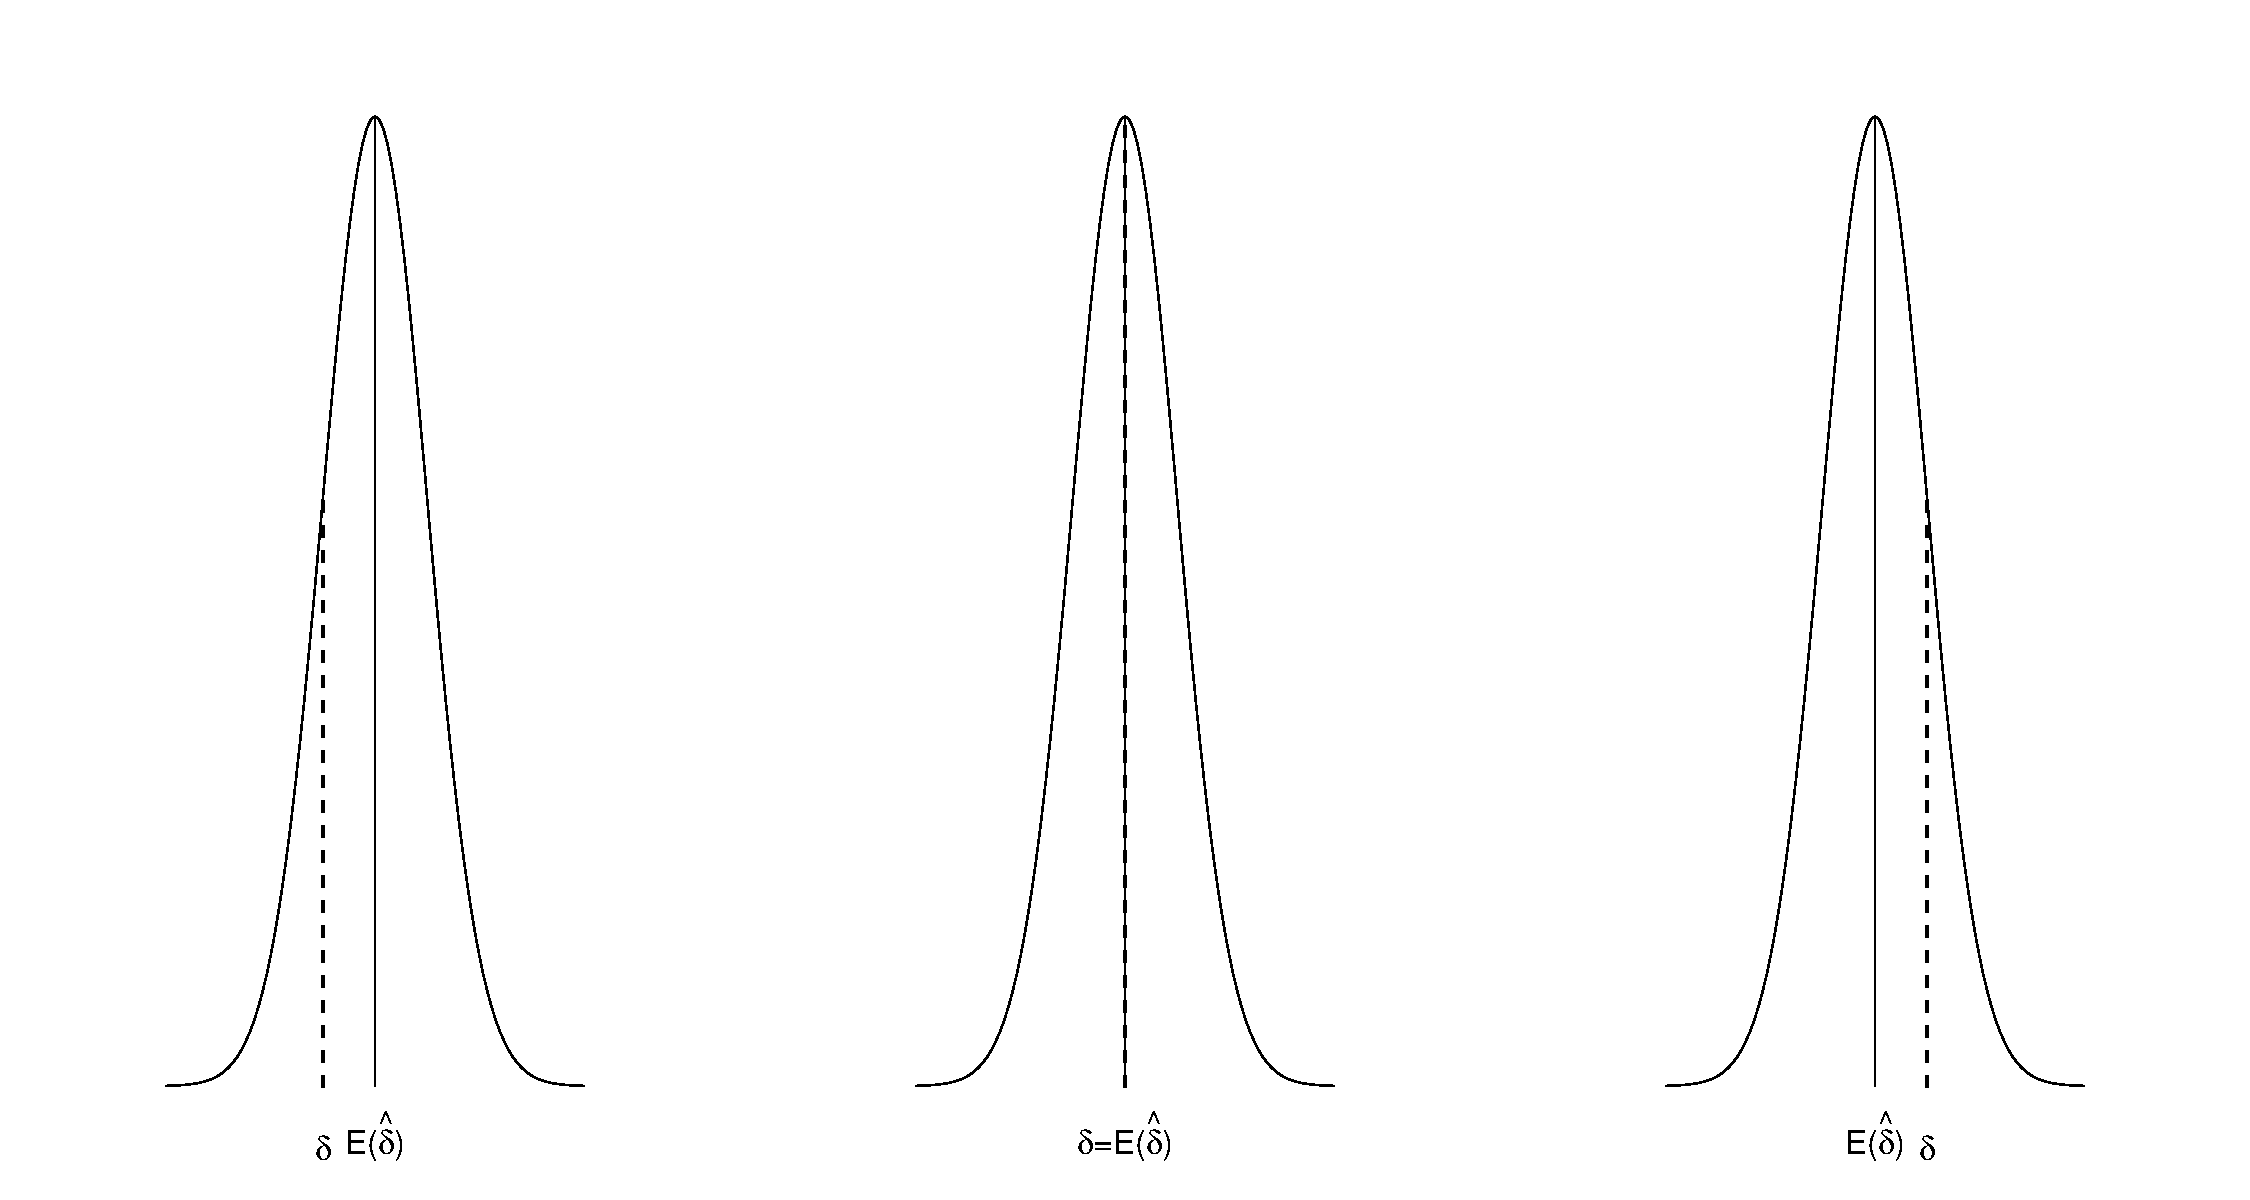
\includegraphics[width=400px]{ES_files/figure-latex/BIAS-1} \caption{Samplig distribution for a positively biased (left), an unbiased (center) and a negatively biased estimator (right)}\label{fig:BIAS}
\end{figure}

Moreover, since there is a strong relationship between the bias and the size of any estimator (the larger an estimator, the larger the bias), it might be interesting to also define the \emph{relative bias} as the ratio between the bias and the population parameter:

\begin{equation} 
\hat{\delta}_{relative \; bias}=\frac{E(\hat{\delta})-\delta}{\delta}
\label{eq:RELBIAS}
\end{equation}

While the bias informs us about the quality of estimates on average, in particular their capacity of lying close to the true value, it says nothing about individual estimates. Imagine a situation where the distribution of estimates is centered around the real parameter but with such a large variance that some point estimates are very far from the center. This would be problematic, since we then do not know if this estimate, based on the sample at hand, is close to the truth or far off. Therefore it is not only essential for an estimator to be unbiased, but the variability of its sampling distribution should also ideally be small. Put simply, we hope that \emph{all} possible estimates are close enough of the true population parameter, in order to be sure that for \emph{any} estimate, one has a correct estimation of the real parameter. Among two unbiased estimators \(\hat{\delta_1}\) and \(\hat{\delta_2}\), we therefore say that \(\hat{\delta_1}\) is \textbf{more efficient} than \(\hat{\delta_2}\) if

\begin{equation} 
Var(\hat{\delta}_1) \leq Var(\hat{\delta}_2)
\label{eq:EFFICIENCY}
\end{equation}

Where \(Var(\hat{\delta})\) is the variance of the sampling distribution of the estimator \(\hat{\delta}\). Among all unbiased estimators, the more efficient will be the one with the smallest variance \footnote{The famous Cr\'amer-Rao inequality provides a theoretical lower bound for the variance of unbiased estimators. An estimator reaching this bound is therefore most efficient.}. Again, the variance of an estimator \(\hat{\delta}\) is a function of its size (the larger the estimator, the larger the variance) and therefore, we might be interested in computing the \emph{relative variance} as the ratio between the variance and the square of the population estimator:

\begin{equation} 
\hat{\delta}_{relative \; variance}=\frac{Var(\hat{\delta})}{\delta^2}
\label{eq:RELVAR}
\end{equation}

Note that both unbiasedness and efficiency are very important. An unbiased estimator with such a large variance that somes estimates are extremely far from the real parameter is as undesirable as a parameter which is highly biased. In some situations, it is better to have a slightly biased estimator with a tight shape around the biased value (so that each estimate remains relatively close to the true parameter and one can apply bias correction techniques) rather than an unbiased estimator with a large variance (Raviv, 2014).

Finally, the last property of a good point estimator is \textbf{consistency}: consistency means that the bigger the sample size, the closer the estimate is to the population parameter. In other words, the estimates \emph{converge} to the true population parameter.

Beyond the inferential properties, Cumming (2013) reminds that an effect size estimator needs to have a constant value across designs in order to be easily interpretable and to be included in meta-analysis. In other words, it should achieve the property of \textbf{generality}.

\hypertarget{confidence-interval-around-a-point-estimator}{%
\section{Confidence interval around a point estimator}\label{confidence-interval-around-a-point-estimator}}

We already mentioned that confidence interval around a point estimate could replace conventional hypothesis testing. A confidence interval contains all the information that a \(p\)-value of a test based on the same estimator does: if the area of the null hypothesis is out of the \((1-\alpha)\)-confidence interval, then the hypothesis test would also result in a \emph{p}-value below the nominal alpha level. Hypothesis tests and confidence intervals based on the same statistical quantity (this is an essential requirement) are thus directly related. At the same time, the intervals provide extra information about the precision of the sample estimate for inferential purposes, and therefore on how confident we can be in the observed results (Altman, 2005; Ellis, 2015): the narrower the interval, the higher the precision. On the other hand, the wider the confidence interval, the more the data lacks precision (for example, because the sample size is too small).

\hypertarget{different-measures-of-effect-sizes}{%
\section{Different measures of effect sizes}\label{different-measures-of-effect-sizes}}

The \emph{d}-family effect sizes are commonly used with \enquote{between-subject} designs where individuals are randomly assigned into one of two independent groups and groups scores means are compared. The population effect size is defined as

\begin{equation} 
\delta = \frac{\mu_{1}-\mu_{2}}{\sigma} 
\label{eq:Cohendelta}
\end{equation}

where both populations follow a normal distribution with mean \(\mu_j\) in the \(j^{th}\) population (j=1,2) and common standard deviation \(\sigma\). They exist different estimators of this effect size measure varying as a function of the chosen standardizer (\(\sigma\)). For all estimators, the mean difference is estimated by the difference \(\bar{X}_1-\bar{X}_2\) of both sample means. When used for inferential purposes, some estimators require both the assumptions of normally distributed data and the equality of variances, while others rely
solely on the assumption of normality. Throughout this section, we will present some of these estimators, separately depending on whether they rely on the assumption of equality of variances or not. For each of them, we will provide information about their theoretical bias, variance and consistency.

\hypertarget{alternatives-when-variances-are-equal-between-groups}{%
\subsection{Alternatives when variances are equal between groups}\label{alternatives-when-variances-are-equal-between-groups}}

\hypertarget{cohens-d_s}{%
\subsubsection{\texorpdfstring{Cohen's \(d_s\)}{Cohen's d\_s}}\label{cohens-d_s}}

When we have good reasons to assume equality of variances between groups, then the most common estimator of \(\delta\) is Cohen's \(d_{s}\) where the sample mean difference is divided by a pooled error term (Cohen, 1965):
\begin{equation} 
Cohen's \; d_s = \frac{\bar{X}_1-\bar{X}_2}{\sqrt{\frac{(n_1-1) \times SD_1+(n_2-1) \times SD_2}{n_1+n_2-2}}} 
\label{eq:Cohends}
\end{equation}

Where \(SD_j\) is the standard deviation and \(n_j\) the sample size of the \(j^{th}\) sample (j=1,2). The reasoning behind this measure is to make use of the fact that both samples share the same population variance (Keselman, Algina, Lix, Deering, \& Wilcox, 2008), hence we achieve a more accurate estimation of the population variance by pooling both estimates of this parameter (i.e \(SD_1\) and \(SD_2\)). Since the larger the sample size, the more accurate the estimate, we give more weight to the estimate based on the larger sample size.

Cohen's \(d_{s}\) is directly related with Student's \emph{t}-test, whose distribution is well known:

\begin{equation} 
t_{student} = cohen's \; d_s \times \sqrt{\frac{n_1n_2}{n_1+n_2}} \sim t_{df,\Delta}
\label{eq:Cohenvsstudent}
\end{equation}

With \(df=n_1+n_2-2\) and \(\Delta = \frac{\mu_1-\mu_2}{\sigma_{pooled}} \times \sqrt{\frac{n_1n_2}{n_1+n_2}}\). The relationship described in equation \ref{eq:Cohenvsstudent} allows us to theoretically determine the sampling distribution of Cohen's \(d_s\), and therefore, its theoretical expectency, bias and variance when the assumptions of normality and equal variances are met. All equations are provided in Table 1. In summary, we can deduce from these equations that:

\begin{itemize}
\tightlist
\item
  When Cohen's \(\delta_s\) is null, the bias is null. In all other configurations, the \textbf{bias} of Cohen's \(d_s\) is a function of total sample size (N) and the population effect size (\(\delta_{Cohen}\)):

  \begin{itemize}
  \tightlist
  \item
    The larger the population effect size, the more Cohen's \(d_s\) will overestimate Cohen's \(\delta_s\).\footnote{Because  $\frac{\sqrt{\frac{N-2}{2}} \times \Gamma(\frac{N-3}{2})}{\Gamma(\frac{N-2}{2})} > 0$}\\
  \item
    The larger the total sample size, the lower the bias. The bias tends to zero when the total sample size tends to infinity.
  \end{itemize}
\item
  The \textbf{variance} of Cohen's \(d_s\) is a function of the population effect size (Cohen's \(\delta_s\)), total sample size and sample sizes allocation ratio :

  \begin{itemize}
  \tightlist
  \item
    The larger the population effect size, the larger the variance.
  \item
    The larger the sample sizes, the lower the variance. The variance tends to zero when the total sample sample size tends to infinity.\\
  \item
    All other parameters beeing equal, the variance is minimized when sample sizes are equal across groups. The larger the sample size allocation ratio, the larger the variance.
  \end{itemize}
\end{itemize}

While Cohen's \(d_s\) is a consistent estimator, its bias and variance are substantial with small sample sizes, even under the assumptions of normality and equal variances (Lakens, 2013).

\hypertarget{hedges-g_s}{%
\subsubsection{\texorpdfstring{Hedge's \(g_s\)}{Hedge's g\_s}}\label{hedges-g_s}}

In order to compensate for Cohen's \(d_s\) bias with small sample sizes, Hedges \& Olkin (1985) has defined a bias-corrected version:

\begin{equation} 
Hedge's \; g_s = Cohen's \; d_s \times \left( \frac{\Gamma(\frac{N-2}{2})}{\sqrt{\frac{N-2}{2}} \times \Gamma(\frac{N-3}{2})} \right)^2
\label{eq:Hedgesgs}
\end{equation}

This equation can be estimated as follows:

\begin{equation} 
Hedge's \; g_s = Cohen's \; d_s \times \left( 1- \frac{3}{4N -9} \right)
\label{eq:Hedgesgsapprox}
\end{equation}

Where N = \(n_1+n_2\). Hedge's \(g_s\) is theoretically unbiased when the assumptions of normality and equal variances are met. Like Cohen's \(d_s\), its variance increases when the sample size allocation ratio and/or the population effect size increases, and decreases when the total sample size increases. However, due to the correction, Hedge's \(g_s\) has a smaller variance than Cohen's \(d_s\), especially with small sample size.\footnote{$\left(\frac{\Gamma(\frac{N-2}{2})}{\sqrt{\frac{N-2}{2}} \times \Gamma(\frac{N-3}{2})} \right)^2$, in the equation of Hedge's $g_s$ variance, is always less than 1, and tends to 1 when the total sample size tends to infinity, meaning that the larger the total sample size, the smaller the difference between the variance of Cohen's $d_s$ and Hedge's $g_s$}.

While the pooled error term is the best choice when variances are equal between groups (Grissom \& Kim, 2001), it may not be well advised for use with data that violate this assumption (Cumming, 2013; Grissom \& Kim, 2001, 2005; Kelley, 2005, 2005; Shieh, 2013). When variances are unequal between groups, the expression in equation \ref{eq:Cohendelta} is no longer valid because both groups don't share a common population variance. If we pool the estimates of two unequal population variances, the estimator of effect size will be lower as it should be in case of positive pairing (i.e.~the group with the larger sample size is extracted from the population with the larger variance) and larger as it should be in case of negative pairing (i.e.~the group with the larger sample size is extracted from the population with the smaller variance). Because the assumption of equal variances across populations is very rare in practice (Cain, Zhang, \& Yuan, 2017; Delacre et al., 2017; Delacre, Leys, Mora, \& Lakens, 2019; Erceg-Hurn \& Mirosevich, 2008; Glass, Peckham, \& Sanders, 1972; Grissom, 2000; Micceri, 1989; Yuan, Bentler, \& Chan, 2004), both Cohen's \(d_s\) and Hedge's \(g_s\) should be abandoned in favor of a robust alternative to unequal population variances.

\newpage
\begin{landscape}

Table 1.
\emph{Expentency, bias and variance of different estimators when the assumption tests are met}

\begin{longtable}[]{@{}lccc@{}}
\toprule
\begin{minipage}[b]{0.06\columnwidth}\raggedright
Estimator\strut
\end{minipage} & \begin{minipage}[b]{0.15\columnwidth}\centering
Expectency\strut
\end{minipage} & \begin{minipage}[b]{0.19\columnwidth}\centering
Bias\strut
\end{minipage} & \begin{minipage}[b]{0.48\columnwidth}\centering
Variance\strut
\end{minipage}\tabularnewline
\midrule
\endhead
\begin{minipage}[t]{0.06\columnwidth}\raggedright
\tiny\(Cohen's \; d_s\)\strut
\end{minipage} & \begin{minipage}[t]{0.15\columnwidth}\centering
\tiny\(\delta_{cohen} \times \frac{\sqrt{\frac{N-2}{2}} \times \Gamma(\frac{N-3}{2})}{\Gamma(\frac{N-2}{2})}\)\strut
\end{minipage} & \begin{minipage}[t]{0.19\columnwidth}\centering
\tiny\(\delta_{cohen} \times \left( \frac{\sqrt{\frac{N-2}{2}} \times \Gamma(\frac{N-3}{2})}{\Gamma(\frac{N-2}{2})}-1 \right)\)\strut
\end{minipage} & \begin{minipage}[t]{0.48\columnwidth}\centering
\tiny\(\frac{N-2}{(N-4) \times \frac{n_1n_2}{N}} \times \left(1+\frac{n_1n_2}{N} \times \delta_{cohen}^2\right) -\delta_{cohen}^2 \times \left[\frac{\sqrt{\frac{N-2}{2}} \times \Gamma(\frac{N-3}{2})}{\Gamma(\frac{N-2}{2})}\right]^2\)\strut
\end{minipage}\tabularnewline
\begin{minipage}[t]{0.06\columnwidth}\raggedright
\strut
\end{minipage} & \begin{minipage}[t]{0.15\columnwidth}\centering
\tiny\(\approx \frac{\delta_{Cohen}}{\left(1-\frac{3}{4N-9}\right)}\)\strut
\end{minipage} & \begin{minipage}[t]{0.19\columnwidth}\centering
\tiny\(\approx \delta_{Cohen} \left[\frac{1}{\left(1-\frac{3}{4N-9}\right)}-1\right]\)\strut
\end{minipage} & \begin{minipage}[t]{0.48\columnwidth}\centering
\tiny\(\approx\frac{N-2}{(N-4) \times \frac{n_1n_2}{N}} \times \left(1+\frac{n_1n_2}{N} \times \delta_{cohen}^2\right) -\delta_{cohen}^2 \times \left[\frac{1}{\left(1-\frac{3}{4N-9}\right)}\right]^2\)\strut
\end{minipage}\tabularnewline
\begin{minipage}[t]{0.06\columnwidth}\raggedright
\strut
\end{minipage} & \begin{minipage}[t]{0.15\columnwidth}\centering
\strut
\end{minipage} & \begin{minipage}[t]{0.19\columnwidth}\centering
\strut
\end{minipage} & \begin{minipage}[t]{0.48\columnwidth}\centering
\strut
\end{minipage}\tabularnewline
\begin{minipage}[t]{0.06\columnwidth}\raggedright
\tiny\(Hedges's \; d_s\)\strut
\end{minipage} & \begin{minipage}[t]{0.15\columnwidth}\centering
\tiny\(\delta_{Cohen}\)\strut
\end{minipage} & \begin{minipage}[t]{0.19\columnwidth}\centering
/\strut
\end{minipage} & \begin{minipage}[t]{0.48\columnwidth}\centering
\tiny\(Var(Cohen's \; d_s) \times \left[ \frac{\Gamma(\frac{N-2}{2})}{\sqrt{\frac{N-2}{2}} \times \Gamma(\frac{N-3}{2})} \right]^2\)\strut
\end{minipage}\tabularnewline
\begin{minipage}[t]{0.06\columnwidth}\raggedright
\strut
\end{minipage} & \begin{minipage}[t]{0.15\columnwidth}\centering
\strut
\end{minipage} & \begin{minipage}[t]{0.19\columnwidth}\centering
\strut
\end{minipage} & \begin{minipage}[t]{0.48\columnwidth}\centering
\tiny\(Var(Cohen's \; d_s) \times \left[1-\frac{3}{4N-9}\right]^2\)\strut
\end{minipage}\tabularnewline
\begin{minipage}[t]{0.06\columnwidth}\raggedright
\strut
\end{minipage} & \begin{minipage}[t]{0.15\columnwidth}\centering
\strut
\end{minipage} & \begin{minipage}[t]{0.19\columnwidth}\centering
\strut
\end{minipage} & \begin{minipage}[t]{0.48\columnwidth}\centering
\strut
\end{minipage}\tabularnewline
\begin{minipage}[t]{0.06\columnwidth}\raggedright
\tiny\(Glass's \; d_s\)\strut
\end{minipage} & \begin{minipage}[t]{0.15\columnwidth}\centering
\tiny\(\delta_{glass} \times \frac{\sqrt{\frac{n_{c}-1}{2}} \times \Gamma(\frac{n_{c}-2}{2})}{\Gamma(\frac{n_{c}-1}{2})}\)\strut
\end{minipage} & \begin{minipage}[t]{0.19\columnwidth}\centering
\tiny\(\delta_{glass} \times \left( \frac{\sqrt{\frac{n_{c}-1}{2}} \times \Gamma(\frac{n_{c}-2}{2})}{\Gamma(\frac{n_{c}-1}{2})}-1 \right)\)\strut
\end{minipage} & \begin{minipage}[t]{0.48\columnwidth}\centering
\tiny\(\frac{n_{c}-1}{n_c-3} \times \left( \frac{1}{n_c} + \frac{\sigma^2_e}{n_e\sigma^2_c} + \delta^2_{glass}\right) -\delta_{glass}^2 \times \left[\frac{\sqrt{\frac{n_{c}-1}{2}} \times \Gamma(\frac{n_{c}-2}{2})}{\Gamma(\frac{n_{c}-1}{2})}\right]^2\)\strut
\end{minipage}\tabularnewline
\begin{minipage}[t]{0.06\columnwidth}\raggedright
\strut
\end{minipage} & \begin{minipage}[t]{0.15\columnwidth}\centering
\strut
\end{minipage} & \begin{minipage}[t]{0.19\columnwidth}\centering
\strut
\end{minipage} & \begin{minipage}[t]{0.48\columnwidth}\centering
\strut
\end{minipage}\tabularnewline
\begin{minipage}[t]{0.06\columnwidth}\raggedright
\tiny\(Shieh's \; d_s\)\strut
\end{minipage} & \begin{minipage}[t]{0.15\columnwidth}\centering
\tiny\(\delta_{Shieh} \times \frac{\sqrt{\frac{df}{2}} \times \Gamma(\frac{df-1}{2})}{\Gamma(\frac{df}{2})}\)\strut
\end{minipage} & \begin{minipage}[t]{0.19\columnwidth}\centering
\tiny\(\delta_{Shieh} \times \left(\frac{\sqrt{\frac{df}{2}} \times \Gamma(\frac{df-1}{2})}{\Gamma(\frac{df}{2})}-1 \right)\)\strut
\end{minipage} & \begin{minipage}[t]{0.48\columnwidth}\centering
\tiny\(\frac{df}{(df-2) \times N} \left( 1+N \times \delta_{Shieh}^2 \right) -\delta_{Shieh}^2 \times \left[\frac{\sqrt{\frac{df}{2}} \times \Gamma(\frac{df-1}{2})}{\Gamma(\frac{df}{2})}\right]^2\)\strut
\end{minipage}\tabularnewline
\begin{minipage}[t]{0.06\columnwidth}\raggedright
\strut
\end{minipage} & \begin{minipage}[t]{0.15\columnwidth}\centering
\strut
\end{minipage} & \begin{minipage}[t]{0.19\columnwidth}\centering
\strut
\end{minipage} & \begin{minipage}[t]{0.48\columnwidth}\centering
\strut
\end{minipage}\tabularnewline
\begin{minipage}[t]{0.06\columnwidth}\raggedright
\strut
\end{minipage} & \begin{minipage}[t]{0.15\columnwidth}\centering
\strut
\end{minipage} & \begin{minipage}[t]{0.19\columnwidth}\centering
\tiny\(with \; df \approx \frac{\left(\frac{\sigma^2_1}{n_1}+\frac{\sigma^2_2}{n_2} \right)^2}{\frac{(\sigma^2_1/n_1)^2}{n_1-1}+\frac{(\sigma^2_2/n_2)^2}{n_2-1}}\)\strut
\end{minipage} & \begin{minipage}[t]{0.48\columnwidth}\centering
\strut
\end{minipage}\tabularnewline
\bottomrule
\end{longtable}

\emph{Note.} N is the total sample size (n1+n2). Equations returns theoretical expectency, bias and variance of Cohen's ds and Hedge's gs under the assumptions that independent residuals are normally distributed with equal variances across groups, as well as theoretical expectency, bias and variance of Glass's ds and Shieh's ds under the assumptions that independent residuals are normally distributed.
\emph{Note.} SPECIFY THAT SOME EQUATIONS ARE UNDEFINED WITH TOO SMALL N. COMPUTING BIAS OF COHEN'S DS REQUIRES THAT N\textgreater=4 (COMPUTING VARIANCES OF COHEN'S DS and HEDGE'S GS REQUIRES THAT N \textgreater=5).

\end{landscape}

\newpage

\hypertarget{alternatives-when-variances-are-unequal-between-populations}{%
\subsection{Alternatives when variances are unequal between populations}\label{alternatives-when-variances-are-unequal-between-populations}}

In his review, Shieh (2013) mentions three options available in the literature to deal with the case of unequal variances: the sample mean difference divided by (A) the non pooled average of both variance estimates, (B) the Glass's \(d_s\) and (C) the Shieh's \(d_s\).

The sample mean difference, divided by the non pooled average of both variance estimates was suggested by Cohen (1988). We immediately exclude this alternative because it suffers from several limitations:\\
- it results in a variance term of an artificial population and is therefore very difficult to interpret (Grissom \& Kim, 2001);\\
- unless both sample sizes are equal, the variance term does not correspond to the variance of the mean difference (Shieh, 2013);\\
- unless the mean difference is null, the measure is biased. Moreover, the bigger the sample size, the larger the variance around the estimate.

\hypertarget{glasss-d_s}{%
\subsubsection{\texorpdfstring{Glass's \(d_s\)}{Glass's d\_s}}\label{glasss-d_s}}

When comparing one control group with one experimental group, Glass, McGav, \& Smith (2005) recommend using the standard deviation \(SD\) of the control group as standardizer. It is also advocated by Cumming (2013), because, according to him, it is what makes the most sense, conceptually speaking. This yields

\begin{equation} 
Glass's \; d_s = \frac{\bar{X}_{e} - \bar{X}_{c}}{SD_{c}}
\label{eq:Glassds}
\end{equation}

Where \(\bar{X}_{e} \; and \; \bar{X}_{c}\) are respectively the sample means of the experimental and control groups, and \(SD_{c}\) is the sample SD of the control group. One argument in favour of using the \(SD\) of the control group as standardizer is the fact that it is not affected by the experimental treatment. When it is easy to identify which group is the \enquote{control} one, it is therefore convenient to compare the effect size estimation of different designs studying the same effect. However, defining this group is not always obvious (Coe, 2002). This could induce large ambiguity because depending of the chosen \(SD\) as standardizer, measures could be substantially different (Shieh, 2013).

Glass's \(d_{s}\) is directly related with a \emph{t} statistic following a known distribution (Algina, Keselman, \& Penfield, 2006):

\begin{equation} 
t = \frac{Glass's \; d_s}{\sqrt{\frac{1}{n_{c}}+\frac{SD_{e}^2}{n_{e} \times SD^2_{c}}}} \sim t_{DF,ncp}
\label{eq:glassvst}
\end{equation}

Where \(DF = n_{c}-1\) and \(ncp = \frac{\mu_{c}-\mu_{e}}{\sigma_{c} \times \sqrt{\frac{1}{n_{c}} + \frac{\sigma_{e}^2}{n_{e} \times \sigma^2_{c}}}}.\) The relationship described in equation \ref{eq:glassvst} allows us to theoretically determine the sampling distribution of Glass's \(d_s\), and therefore, its theoretical expectency, bias and variance under the assumption of normality (see Table 1). In summary, we can deduce from these equations that:

\begin{itemize}
\item
  When Glass's \(\delta_s\) is null, the bias is null. In all other configurations, the \textbf{bias} of Glass's \(d_s\) is a function of the sample size of the control group (\(n_c\)) and the population effect size (\(\delta_{glass}\)):

  \begin{itemize}
  \tightlist
  \item
    The larger the population effect size, the more Glass's \(d_s\) will overestimate Glass's \(\delta_s\).\footnote{Because  $\frac{\sqrt{\frac{n_c-1}{2}} \times \Gamma(\frac{n_c-2}{2})}{\Gamma(\frac{n_c-1}{2})}-1 > 0$}\\
  \item
    The larger the sample size of the control group, the lower the bias. The bias tends to zero when the sample size of the control group tend to infinity.
  \end{itemize}
\item
  The \textbf{variance} of Glass's \(d_s\) is a function of the population effect size (Cohen's \(\delta_s\)), the total sample size and the sample sizes and variance pairing:

  \begin{itemize}
  \tightlist
  \item
    The larger the population effect size, the larger the variance.\\
  \item
    The larger the total sample size, the lower the variance.\\
  \item
    For a constant total sample size (N), the impact of the sample sizes allocation ratio will depend on the SD-ratio.

    \begin{itemize}
    \tightlist
    \item
      When variances are equal across groups, mieux vaut avoir un peu plus de sujets dans le groupe contrôle que dans le groupe experimental (tout en gardant un ratio relativement proche de 1 sinon la variance augmente à nouveau)
    \item
      When the variance of the control group is larger than the variance of the experimental group, rajouter des sujets dans le groupe experimental ne change pratiquement pas la variance. Mieux vaut donc avoir un max de gens dans le groupe contrôle.
    \item
      When the variance of the experimental group is larger than the variance of the control group, il vaut mieux avoir plus de sujets dans le groupe experimental (c'est la cata si le groupe contrôle est le plus grand).
    \end{itemize}
  \end{itemize}
\end{itemize}

Under the assumptions of normality, because the bias of Glass's \(d_s\) does not depend either on the size of the experimental group or on the total sample size, it will decrease only when subjects are added in the control group (i.e.~when \(n_c\) increases), and it will do so more slowly than the bias of Cohen's \(d_s\). Moreover, while the variance of Glass's \(d_s\) decreases when the total sample size increases, it will never tend to zero when sample sizes tend to infinity. For this reason, Glass's \(d_s\) is not a consistent estimator.

\begin{itemize}
\tightlist
\item
  When designs are balanced, the lower the ratio \(\frac{\sigma^2_e}{\sigma^2_c}\), the lower the variance. In other word, the estimator is less variable when choosing the estimate of the largest population SD as standardizer.
\end{itemize}

\hypertarget{shiehs-d_s}{%
\subsubsection{\texorpdfstring{Shieh's \(d_s\)}{Shieh's d\_s}}\label{shiehs-d_s}}

Kulinskaya \& Staudte (2007) were the first to advice the use of a standardizer that take the sample sizes allocation ratios into account, in addition to the variance of both samples. Shieh (2013), following Kulinskaya \& Staudte (2007), proposed a modification of the exact \emph{SD} of the sample mean difference:

\begin{equation} 
Shieh's \; d_s = \frac{\bar{X}_1 - \bar{X}_2}{\sqrt{SD_1^2/q_1+SD_2^2/q_2}}; \;\;\; q_j=\frac{n_j}{N} (j=1,2)
\label{eq:Shiehds}
\end{equation}

where \(N = n_1+n_2\). Shieh's \(d_{s}\) is directly related with Welch's \emph{t}-test. The exact distribution of Welch's \emph{t} statistic is more complicated than the exact distribution of Student's \emph{t} statistic, but it can be approximated (Shieh, 2013; Welch, 1938):

\begin{equation} 
t_{welch} = Shieh's \; d_s \times \sqrt{N} \sim t_{v,\Delta*}
\label{eq:shiehvswelch}
\end{equation}

With \(N = n_1+n_2\), \(v \approx \frac{\left(\frac{\sigma^2_1}{n_1}+\frac{\sigma^2_2}{n_2} \right)^2}{\frac{(\sigma^2_1/n_1)^2}{n_1-1}+\frac{(\sigma^2_2/n_2)^2}{n_2-1}}\) and \(\Delta* = \frac{\mu_1-\mu_2}{\sqrt{\frac{\sigma_1^2}{n_1/N}+\frac{\sigma_2^2}{n_2/N}}} \times \sqrt{N}\). Again, the relationship described in equation \ref{eq:shiehvswelch} allows us to theoretically determine the sampling distribution of Shieh's \(d_s\), and therefore, its theoretical expectency, bias and variance under the assumption of normality (see Table 1). It can be demonstrated that when variances and sample sizes are equal across groups, the biases and variances of Shieh's \(d_s\) and Cohen's \(d_s\) are identical except for a constant, as shown in equations \ref{eq:biascohenshieh} and \ref{eq:varcohenshieh}:

\newpage

Considering \(\sigma_1 = \sigma_2\) and \(n_1 = n_2\):

\begin{equation} 
Shieh's \; d_{s,bias} = 2 \times Cohen's \; d_{s,bias}
\label{eq:biascohenshieh}
\end{equation}

\begin{equation} 
Shieh's \; d_{s,variance} = 4 \times Cohen's \; d_{s,variance}
\label{eq:varcohenshieh}
\end{equation}

Due to the relation described in equation \ref{eq:cohenshieh} when sample sizes are equal between groups (as explained in Appendix 1), such proportions mean that relative to their respective true effect size, Cohen's \(d_s\) and Shieh's \(d_s\) are equally good.

\begin{equation} 
Shieh's \; \delta_{n_1=n_2}= \frac{Cohen's \; \delta_{n_1=n_2}}{2}
\label{eq:cohenshieh}
\end{equation}

Except for this very specific situation, the bias and variance of Shieh's \(d_s\) also depend on sample variances of both groups. According to the statistical properties of Welch's statistic under heteroscedasticity, it does not appear possible to define a proper standardised effect size without accounting for the relative group size of subpopulations in a sampling scheme. At the same time, the lack of generality caused by taking this specificity of the design into account has led Cumming (2013) to question its usefulness in terms of interpretability: when keeping constant the mean difference (\(\bar{X_1}-\bar{X_2}\)) as well as \(SD_1\) and \(SD_2\), Shieh's \(d_s\) will vary as a function of the sample sizes allocation ratio (the dependency of Shieh's \(d_s\) value on the sample sizes allocation ratio is detailed and illustrated in Appendix 1, and also in the following shiny application: \url{https://mdelacre.shinyapps.io/improve-the-interpretability-of-shieh-s-d-shiny-app/}).

Fortunately, this apparent paradox can be resolved. It is possible to find a modified measure of Shieh's \(d_s\) that does not depend on sample sizes ratio, namely by answering the following question: \enquote{whatever the real sample sizes ratio, what value of Shieh's \(d_s\) would have been computed if design were balanced (i.e.~\(n_1 = n_2\)), keeping all other parameters constant?}

It can be shown that the relationship between Shieh's \(\delta\) when samples sizes are equal between groups and Shieh's \(\delta\) for any other sample sizes allocation ratios can be expressed as follows:

\begin{equation} 
Shieh's \; \delta_{n_1=n_2}= Shieh's \; \delta \times \frac{(nratio+1) \times \sigma_{n_1 \neq n_2}}{2 \times \sigma_{n_1=n_2} \times \sqrt{nratio}}
\label{eq:shiehvsbaldesignPOP}
\end{equation}

with \[nratio= \frac{n_1}{n_2}\]
\[\sigma_{n_1=n_2}= \sqrt{\frac{\sigma_1^2+\sigma_2^2}{2}}\]\\
\[\sigma_{n_1 \neq n_2} = \sqrt{(1- \frac{n_1}{N}) \times \sigma_1^2+(1- \frac{n_2}{N}) \times \sigma_2^2}\]

\(Shieh's \; \delta_{n_1=n_2}\) can thefore be estimated using this equation:

\begin{equation} 
Shieh's \; d^*_s= Shieh's \; d_s \times \frac{(nratio+1) \times SD_{n_1 \neq n_2}}{2 \times SD_{n_1=n_2} \times \sqrt{nratio}}
\label{eq:shiehvsbaldesign}
\end{equation}

with \[SD_{n_1=n_2}= \sqrt{\frac{SD_1^2+SD_2^2}{2}}\] and
\[SD_{n_1 \neq n_2} = \sqrt{(1- \frac{n_1}{N}) \times SD_1^2+(1- \frac{n_2}{N}) \times SD_2^2}\]

\(Shieh's \; d^*_s\) can be compared across two different studies using different sample sizes allocation ratio and could thus be included in meta-analysis. As we are the first to propose this solution, we will test its proporties through Monte Carlo simulations.

\hypertarget{monte-carlo-simulations}{%
\subsection{Monte Carlo Simulations}\label{monte-carlo-simulations}}

\hypertarget{simulation-1-assessing-the-bias-efficiency-and-consistency-of-5-estimators}{%
\subsubsection{Simulation 1: assessing the bias, efficiency and consistency of 5 estimators}\label{simulation-1-assessing-the-bias-efficiency-and-consistency-of-5-estimators}}

\hypertarget{method}{%
\paragraph{Method}\label{method}}

We performed Monte Carlo simulations using R (version 3.5.0) to assess the bias, efficiency and consistency of Cohen's \(d_s\), Hedge's \(g_s\), Glass's \(d_s\) (using respectively the sample \(SD\) of the first or second group as a standardizer), Shieh's \(d_s\) and our transformed measure of Shieh's \(d_s\), that we will note later \(d_s^*\). For Hedge's \(g_s\), we used the approximed formula introduced in equation \ref{eq:Hedgesgsapprox}.

A set of 100,000 datasets were generated for 1,008 scenarios as a function of different criterions that will be explained below. In 252 scenarios, samples were extracted from a normally distributed population and in 756 scenarios, samples were extracted from non normal population distributions. In order to assess the quality of estimators under realistic deviations from the normality assumption, we referred to the review of Cain et al. (2017). Cain et al.~(2017) investigated 1,567 univariate distributions from 194 studies published by authors in Psychological Science (from January 2013 to June 2014) and the American Education Research Journal (from January 2010 to June 2014). For each distribution, they computed the Fisher's skewness (G1) and kurtosis (G2):
\begin{equation} 
G_{1}=\frac{\sqrt{n(n-1)}}{n-2} \frac{m_{3}}{\sqrt{(m_{2})^3}}
\label{eq:skew}
\end{equation}

with s = standard deviation, n = sample size, \(m_{2}\) = second centered moment and \(m_{3}\) = third centered moment.

\begin{equation} 
G_{2}=\frac{n-1}{(n-2)(n-3)}\times [(n+1)(\frac{m_{4}}{(m_{2})^2}-3)+6]
\label{eq:kurt}
\end{equation}

with s = standard deviation, n = sample size and \(m_{3}\)=third centered moment. They found values of kurtosis from G2 = -2.20 to 1,093.48. According to their suggestions, throughout our simulations, we kept constant the population kurtosis value at the 99th percentile of their distribution of kurtosis, i.e.~G2=95.75. Regarding skewness, we simulated population parameter values which correspond to the 1st and 99th percentile of their distribution of skewness, i.e.~respectively G1 = -2.08 and G1 = 6.32. We also simulated samples extracted from population where G1 = 0, in order to assess the main effect of high kurtosis on the quality of estimators. All possible combinations of population skewness and kurtosis and the number of scenarios for each combination are summarized in Table 2.

Table 2.
\emph{Number of Combinations of skewness and kurtosis in our simulations}

\begin{longtable}[]{@{}ccccc@{}}
\toprule
& & & \textbf{Kurtosis} &\tabularnewline
\midrule
\endhead
& & 0 & 95.75 & \textbf{TOTAL}\tabularnewline
& & --------------- & -------------- & ---------------\tabularnewline
& 0 & 252 & 252 & \textbf{504}\tabularnewline
& & & &\tabularnewline
\textbf{Skewness} & -2.08 & / & 252 & \textbf{252}\tabularnewline
& & & &\tabularnewline
& 6.32 & / & 252 & \textbf{252}\tabularnewline
& & & &\tabularnewline
& \textbf{TOTAL} & \textbf{252} & \textbf{756} & \textbf{1008}\tabularnewline
\bottomrule
\end{longtable}

\emph{Note.} Fisher's skewness (G1) and kurtosis (G2) are presented in Table 2. The 252 combinations where both G1 and G2 equal 0 correspond to the normal case.

For the 4 resulting combinations of skewness and kurtosis (see Table 2), all other parameter values were chosen in order to illustrate the consequences of factors known to play a key role on quality of estimators. We manipulated the population mean difference (\(\mu_1-\mu_2\)), the sample sizes (\emph{n}), the sample size ratio (\emph{n}-ratio = \(\frac{n_1}{n_2}\)), the population \emph{SD}-ratio (i.e.~\(\frac{\sigma_1}{\sigma_2}\)), and the sample size and population variance pairing. In our scenarios, \(\mu_2\) was always 0 and \(\mu_1\) varied from 1 to 4, in step of 1 (so does \(\mu_1-\mu_2\))\footnote{In the original plan, we had added 252 simulations in which mu1 and mu2 were both null. We decided to not present the results of these simulations, because the relative bias and the relative variance appeared to us to be very useful to fully understand the estimators comparison, and computing them is impossible when the real mean difference is zero.}. Moreover, \(\sigma_1\) always equals 1, and \(\sigma_2\) equals .1, .25, .5, 1, 2, 4 or 10 (so does \(\frac{\sigma_1}{\sigma_2}\)). The simulations for which both \(\sigma_1\) and \(\sigma_2\) equal 1 are the particular case of homoscedasticity (i.e.~equal population variances across groups). Sample size of both groups (\(n_1\) and \(n_2\)) were 20, 50 or 100. When sample sizes of both groups are equal, the \emph{n}-ratio equals 1 (it is known as a balanced design). All possible combinations of \emph{n}-ratio and population \emph{SD}-ratio were performed in order to distinguish positive pairings (the group with the largest sample size is extracted from the population with the largest \emph{SD}), negative pairings (the group with the smallest sample size is extracted from the population with the smallest \emph{SD}), and no pairing (sample sizes and/or population \emph{SD} are equal across all groups). In sum, the simulations grouped over different sample sizes yield 5 conditions based on the \emph{n}-ratio, population \emph{SD}-ratio, and sample size and population variance pairing, as summarized in Table 3.

Table 3.
\emph{5 conditions based on the n-ratio, SD-ratio, and sample size and variance pairing}

\begin{longtable}[]{@{}ccccc@{}}
\toprule
& & & \textbf{\emph{n}-ratio} &\tabularnewline
\midrule
\endhead
& & \textbf{1} & \textbf{\textgreater1} & \textbf{\textless1}\tabularnewline
& & ------------ & ------------- & -------------\tabularnewline
& \textbf{1} & a & b1 & b2\tabularnewline
& & & &\tabularnewline
\textbf{\emph{SD}-ratio} & \textbf{\textgreater1} & c1 & d1 & e1\tabularnewline
& & & &\tabularnewline
& \textbf{\textless1} & c2 & e2 & d2\tabularnewline
\bottomrule
\end{longtable}

\emph{Note.} The \emph{n}-ratio is the sample size of the first group (\(n_1\)) divided by the sample size of the second group (\(n_2\)). When all sample sizes are equal across groups, the \emph{n}-ratio equals 1. When \(n_1 > n_2\), \emph{n}-ratio \textgreater{} 1, and when \(n_1 < n_2\), \emph{n}-ratio \textless{} 1. \emph{SD}-ratio is the population \emph{SD} of the first group (\(\sigma_1\)) divided by the population \emph{SD} of the second group (\(\sigma_2\)). When \(\sigma_1=\sigma_2\), \emph{SD}-ratio = 1. When \(\sigma_1>\sigma_2\), \emph{SD}-ratio \textgreater{} 1. Finally, when \(\sigma_1<\sigma_2\), \emph{SD}-ratio \textless{} 1.
QUESTION: EST-CE-VRAIMENT NECESSAIRE DE DIRE CECI? REP MARIE: JE PENSE QUE oui, POUR NE PAS ETRE OBLIGE DE RETOURNER VOIR DANS LE TEXTE CE QUI CORRESPOND A QUOI.

\hypertarget{results}{%
\paragraph{Results}\label{results}}

Before detailing estimators comparison for each condition, it might be interesting to make some general comments.

\begin{enumerate}
\def\labelenumi{\arabic{enumi})}
\item
  When the normality assumption is met (i.e.~when G1 and G2 = 0, left in Figures 3 to 7), bias and variance of all estimators are quite small. However, the further from the normality assumption (i.e.~when moving from left to right in Figures 3 to 7), the larger the value of all envisaged indicators of quality (i.e.~bias, relative bias, efficiency and relative efficiency). Note that in a purpose of readability, the ordinate axis is not on the same scale depending on the combination G1/G2. However, if the distribution shape influences all our indicators of quality, most of the time, there is no appearant interaction effect between estimators and distribution shape: the general appearance of barplots is almost always the same for all combinations of skewness and kurtosis (the only exception is for the Glass's \(d_s\) when population distributions are skewed, as it will be described later). As a conclusion, the further from the normality assumption, the larger the below mentioned differences between estimators.
\item
  The fact that the bias of all estimators is very small when the normality assumption is met does not mean that all estimators are relevant in any conditions when the normality assumption is met. Because of the pooled error term, Cohen's \(d_s\) and Hedge's \(d_g\) should be avoided when population variances and sample sizes are unequal across groups, as reminded in the section \enquote{Different mesures of effect size}. When pooling the estimates of two unequal population variances, the resulting estimator will be lower (in case of positive pairing) or larger (in case of negative pairing) as it should be. At the same time, when pooling two unequal population variances, the population effect size will also be lower (in case of positive pairing) or larger (in case of negative pairing) as it should be. As a consequence, the distorsion cannot be seen through the difference between the expected estimator and the population effect size measure. In other words, the distorsion cannot be seen through the bias (bias =\(E(\hat{\delta})-\delta\)).
\item
  Throughout this section, we will \textbf{compare} the quality of different estimators. We chose very extreme (although realistic) conditions, and we know that none of the parametric measures of effect size will be robust against such extreme conditions. Our goal is therefore to study the robustness of the estimators against normality violations only in comparison with the robustness of other indicators, but not in absolute terms.
\end{enumerate}

After these general remarks, we will analyze each condition separately. In all Figures presented below, averaged results for each sub-condition are presented under five different configurations of distributions, using the legend described in Figure \ref{fig:legend}. When describing the Glass's \(d_s\) estimators, we will systematically call \enquote{control group} the group the standardizer is computed from (i.e.~the first group when using \(SD_1\) as standardizer, the second group when using \(SD_2\) as standardizer). The other group will be called \enquote{experimental group}.

\begin{figure}
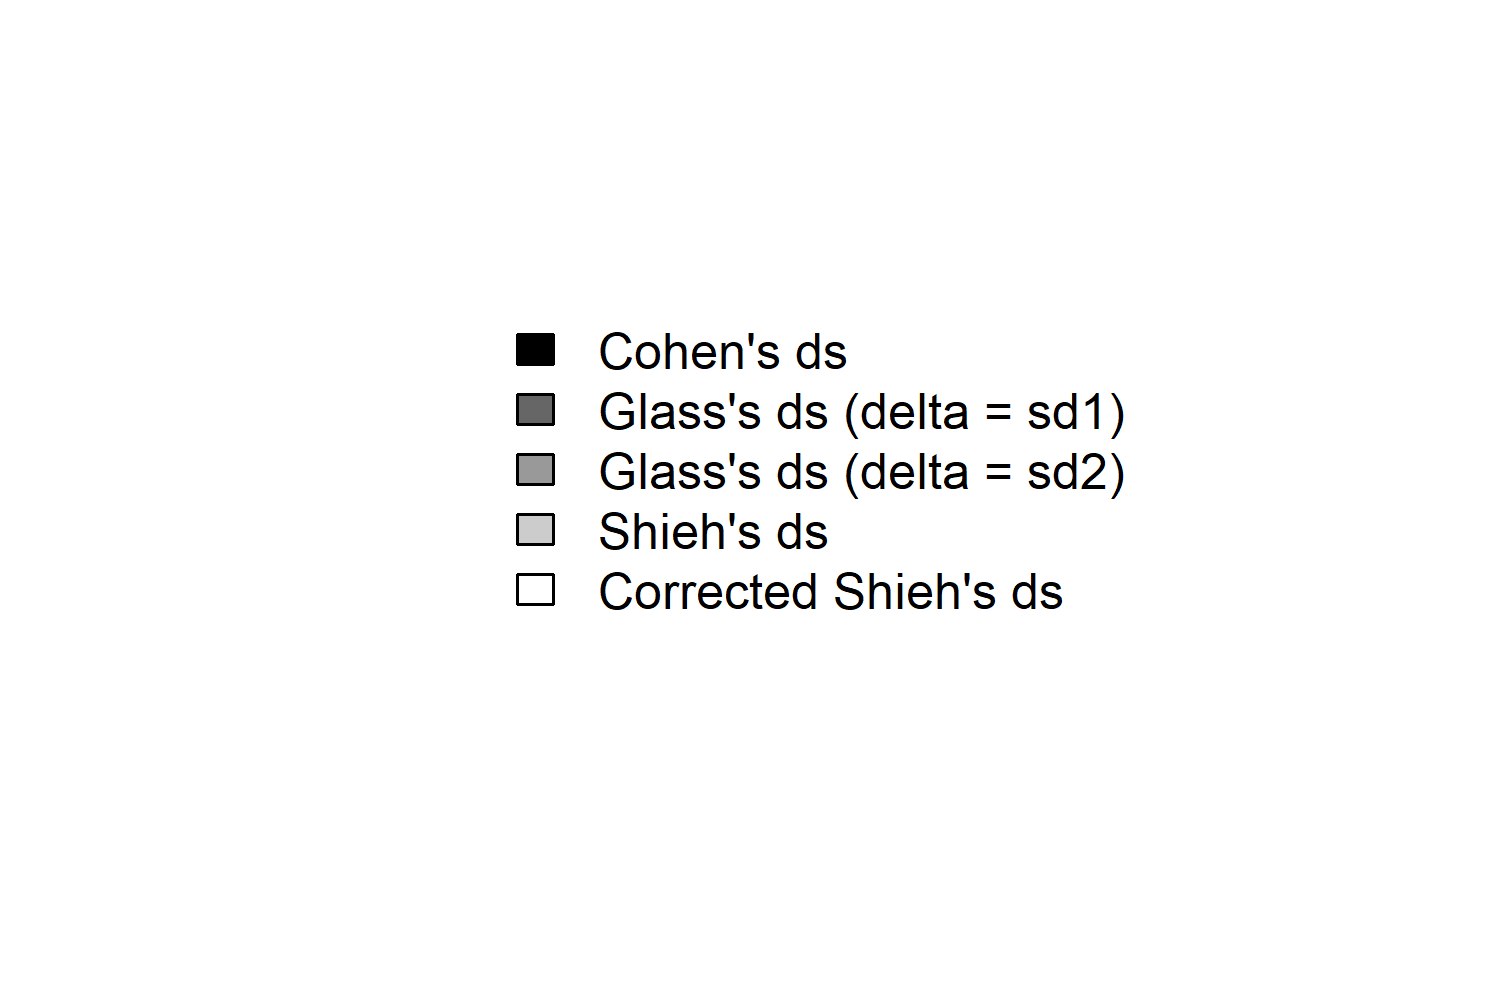
\includegraphics[width=400px]{C:/Users/Marie/Documents/Github_projects/Effect-sizes/Scripts outputs/Quality of ES measures/Graphs/legend} \caption{Legend}\label{fig:legend}
\end{figure}

\hypertarget{when-variances-are-equal-across-groups}{%
\subparagraph{When variances are equal across groups}\label{when-variances-are-equal-across-groups}}

\begin{sidewaysfigure}

{\centering 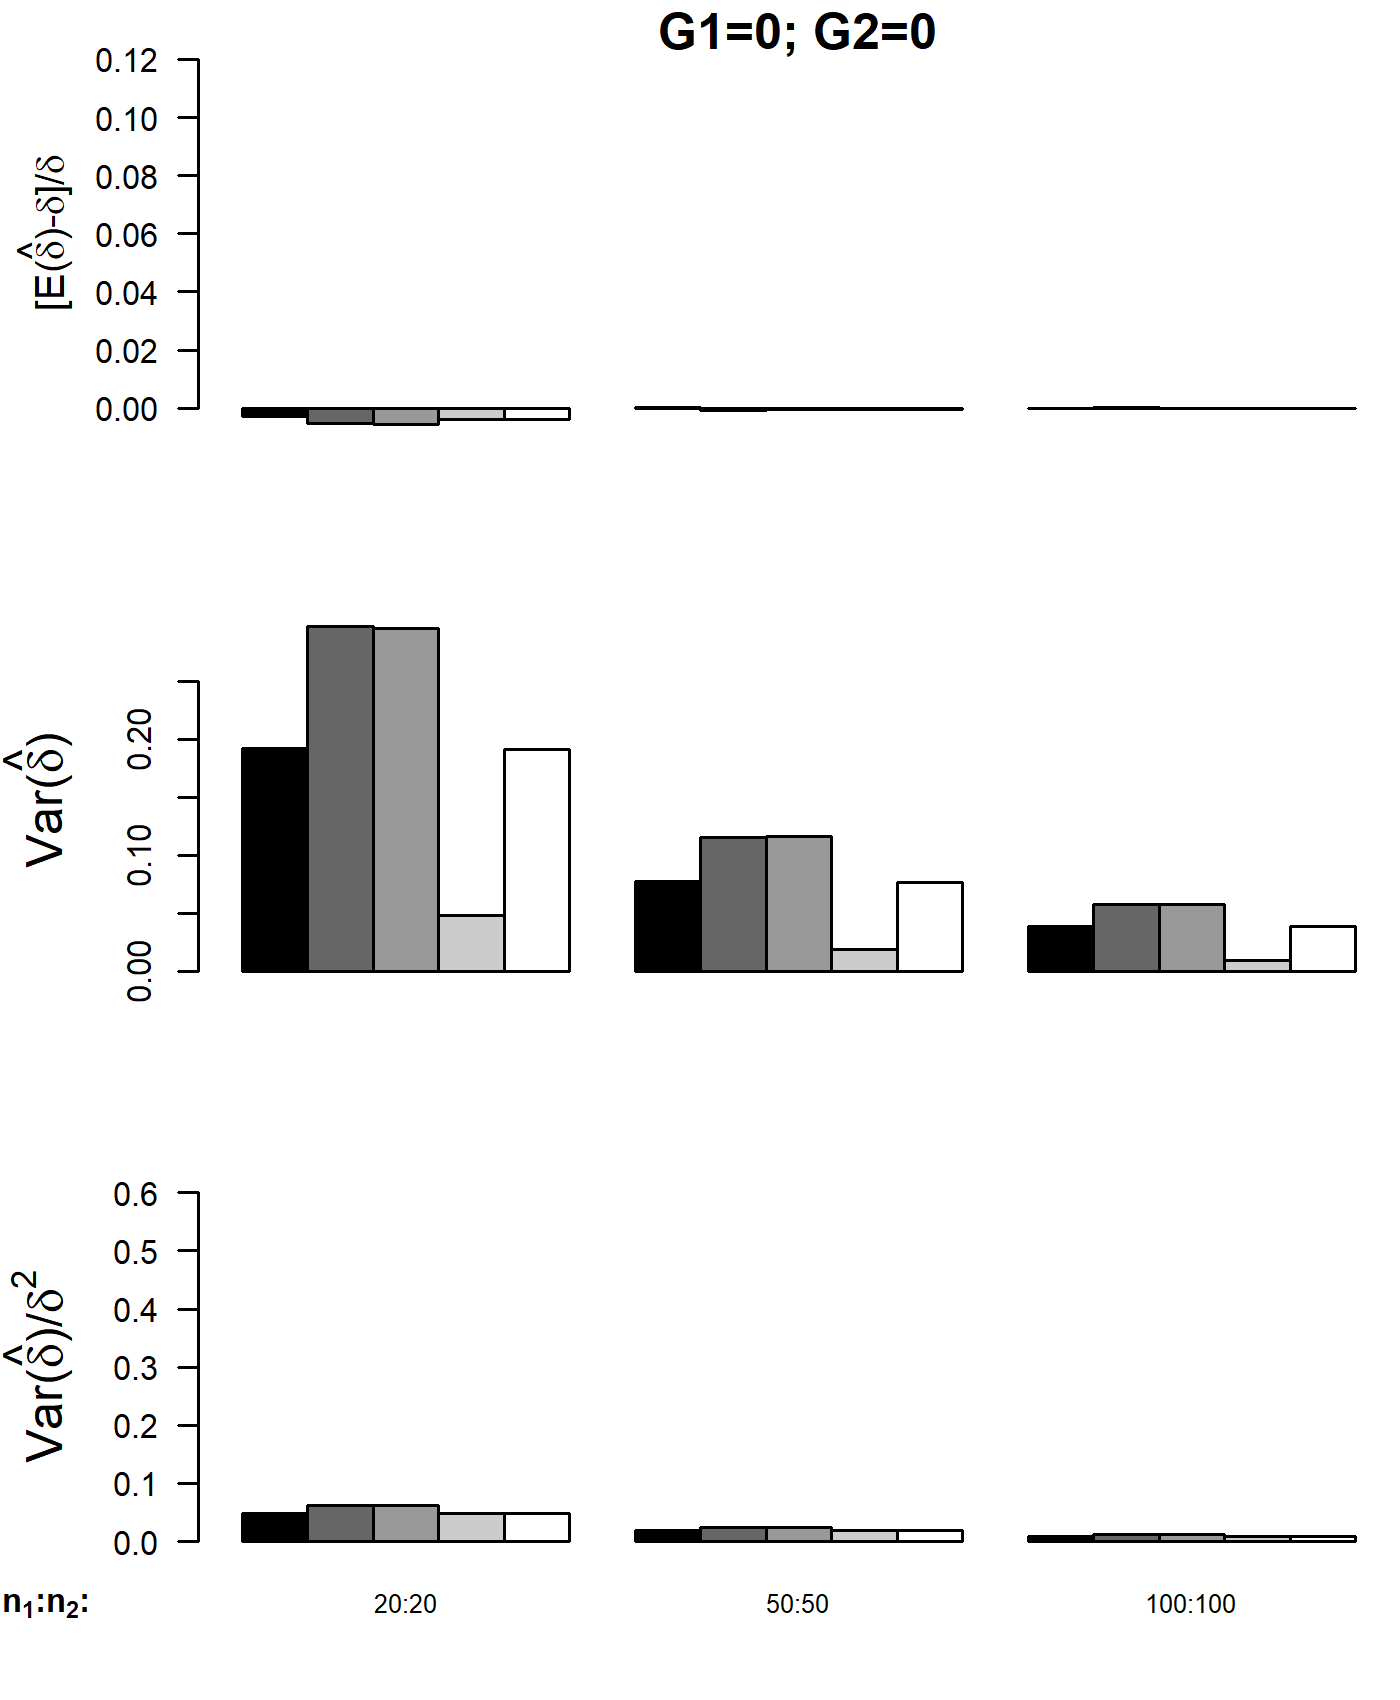
\includegraphics[width=0.2\linewidth]{C:/Users/Marie/Documents/Github_projects/Effect-sizes/Scripts outputs/Quality of ES measures/Graphs/id_Hom_bal/bias_eff,G1=0 & G2=0;id_Hom_bal} 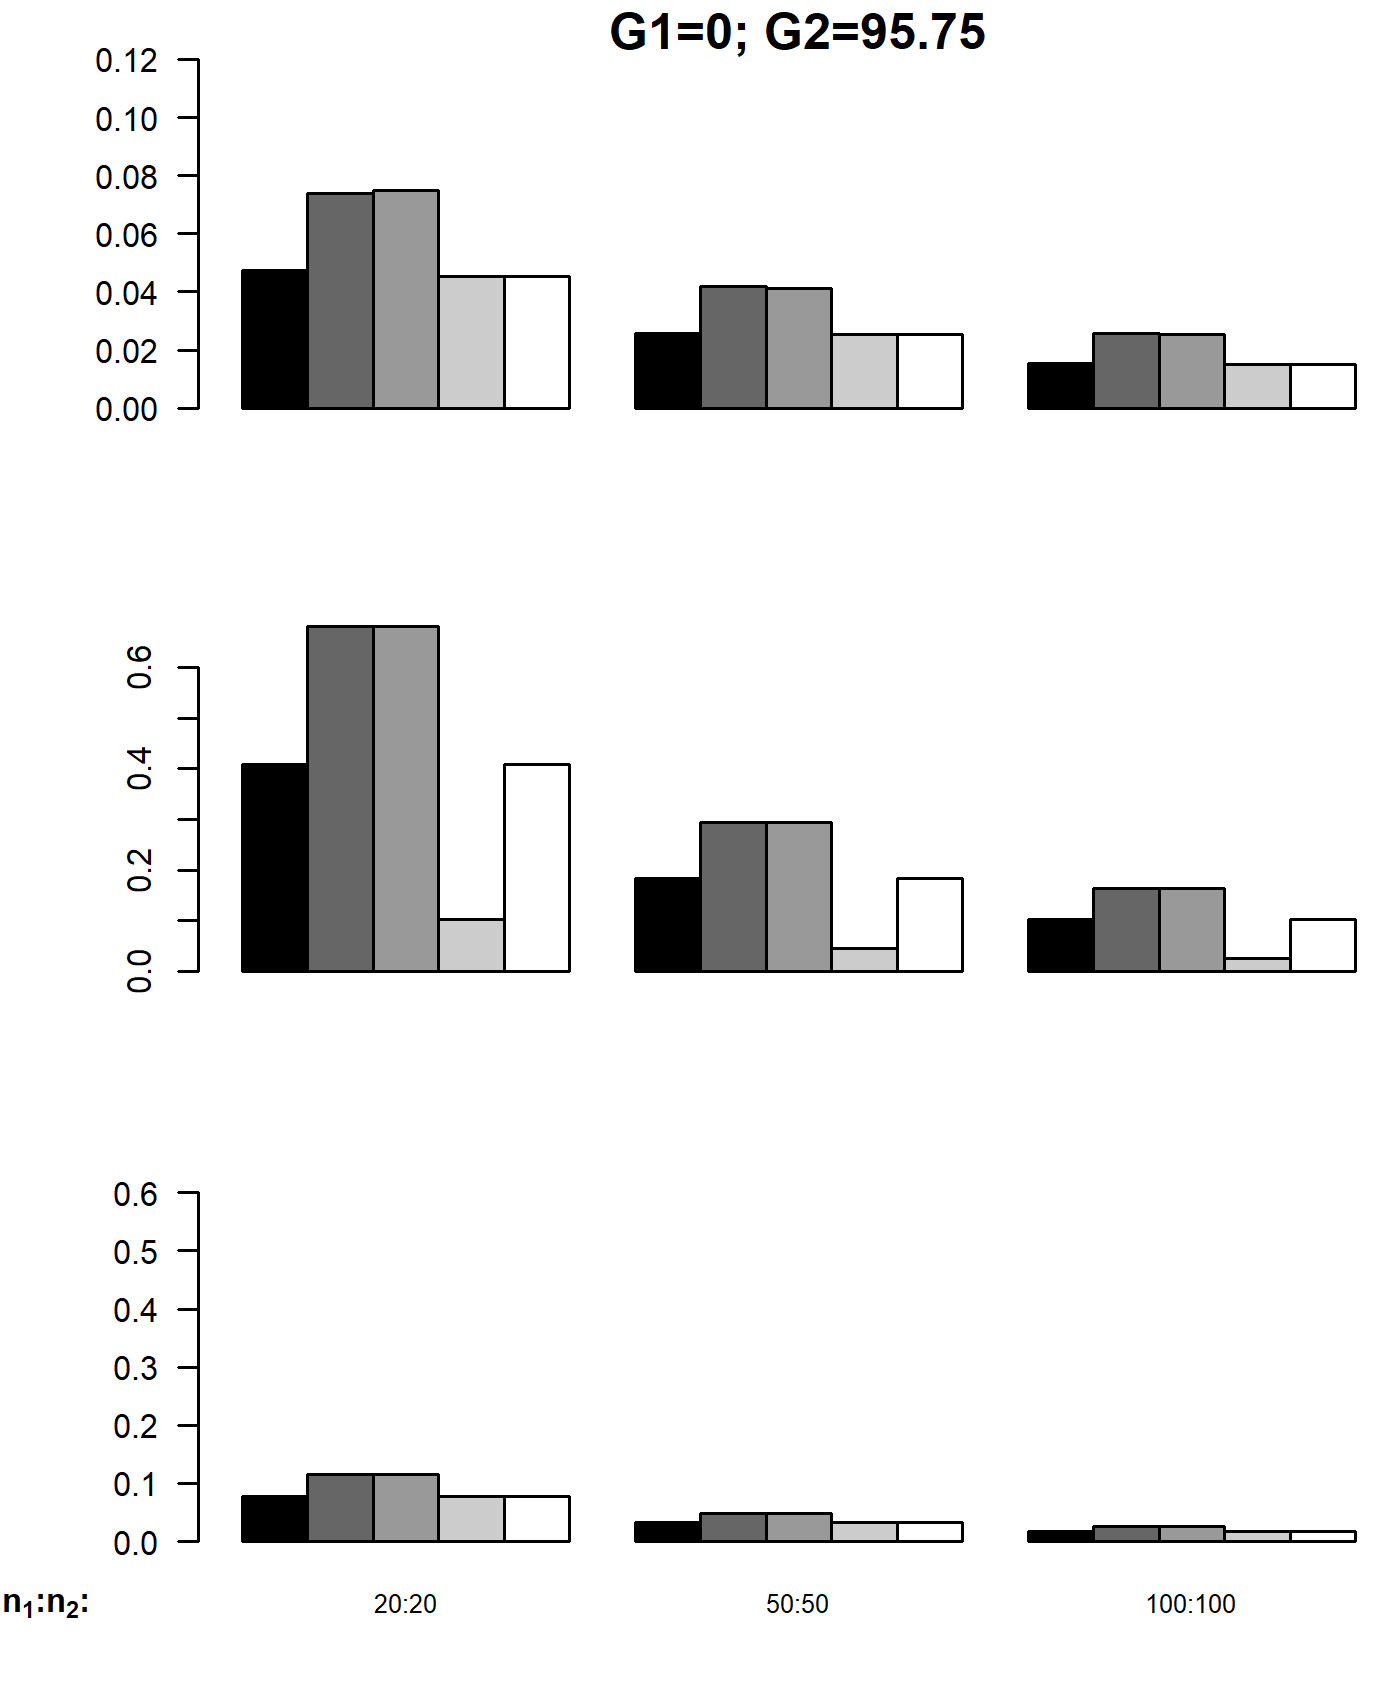
\includegraphics[width=0.2\linewidth]{C:/Users/Marie/Documents/Github_projects/Effect-sizes/Scripts outputs/Quality of ES measures/Graphs/id_Hom_bal/bias_eff,G1=0 & G2=95.75;id_Hom_bal} 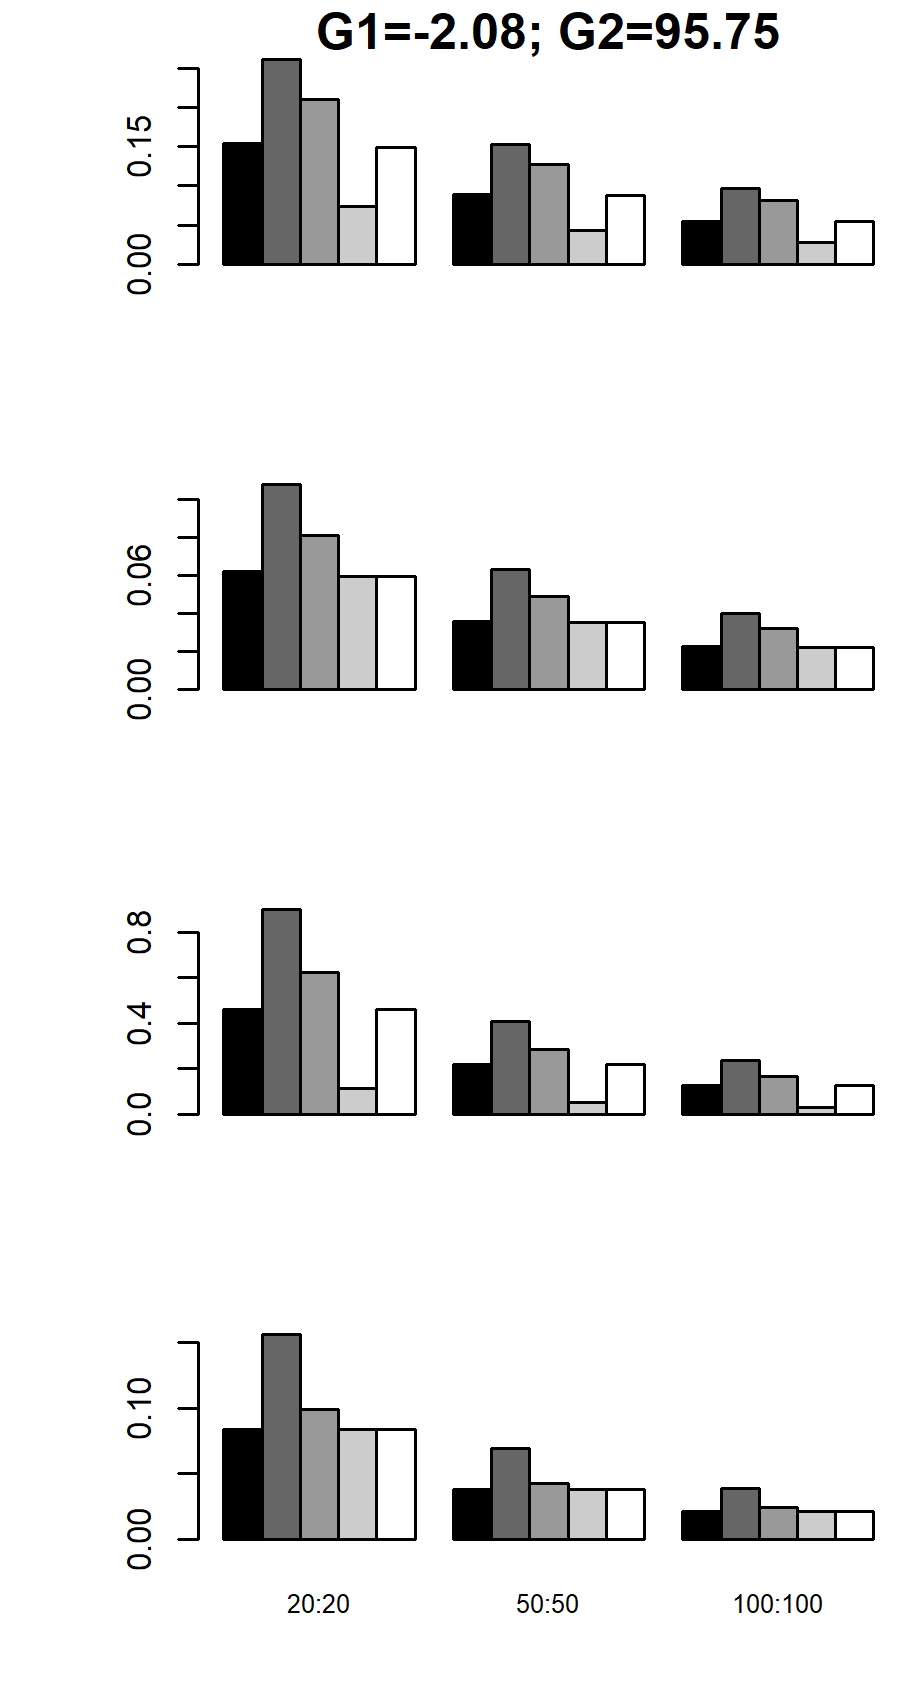
\includegraphics[width=0.2\linewidth]{C:/Users/Marie/Documents/Github_projects/Effect-sizes/Scripts outputs/Quality of ES measures/Graphs/id_Hom_bal/bias_eff,G1=2.08 & G2=95.75;id_Hom_bal} 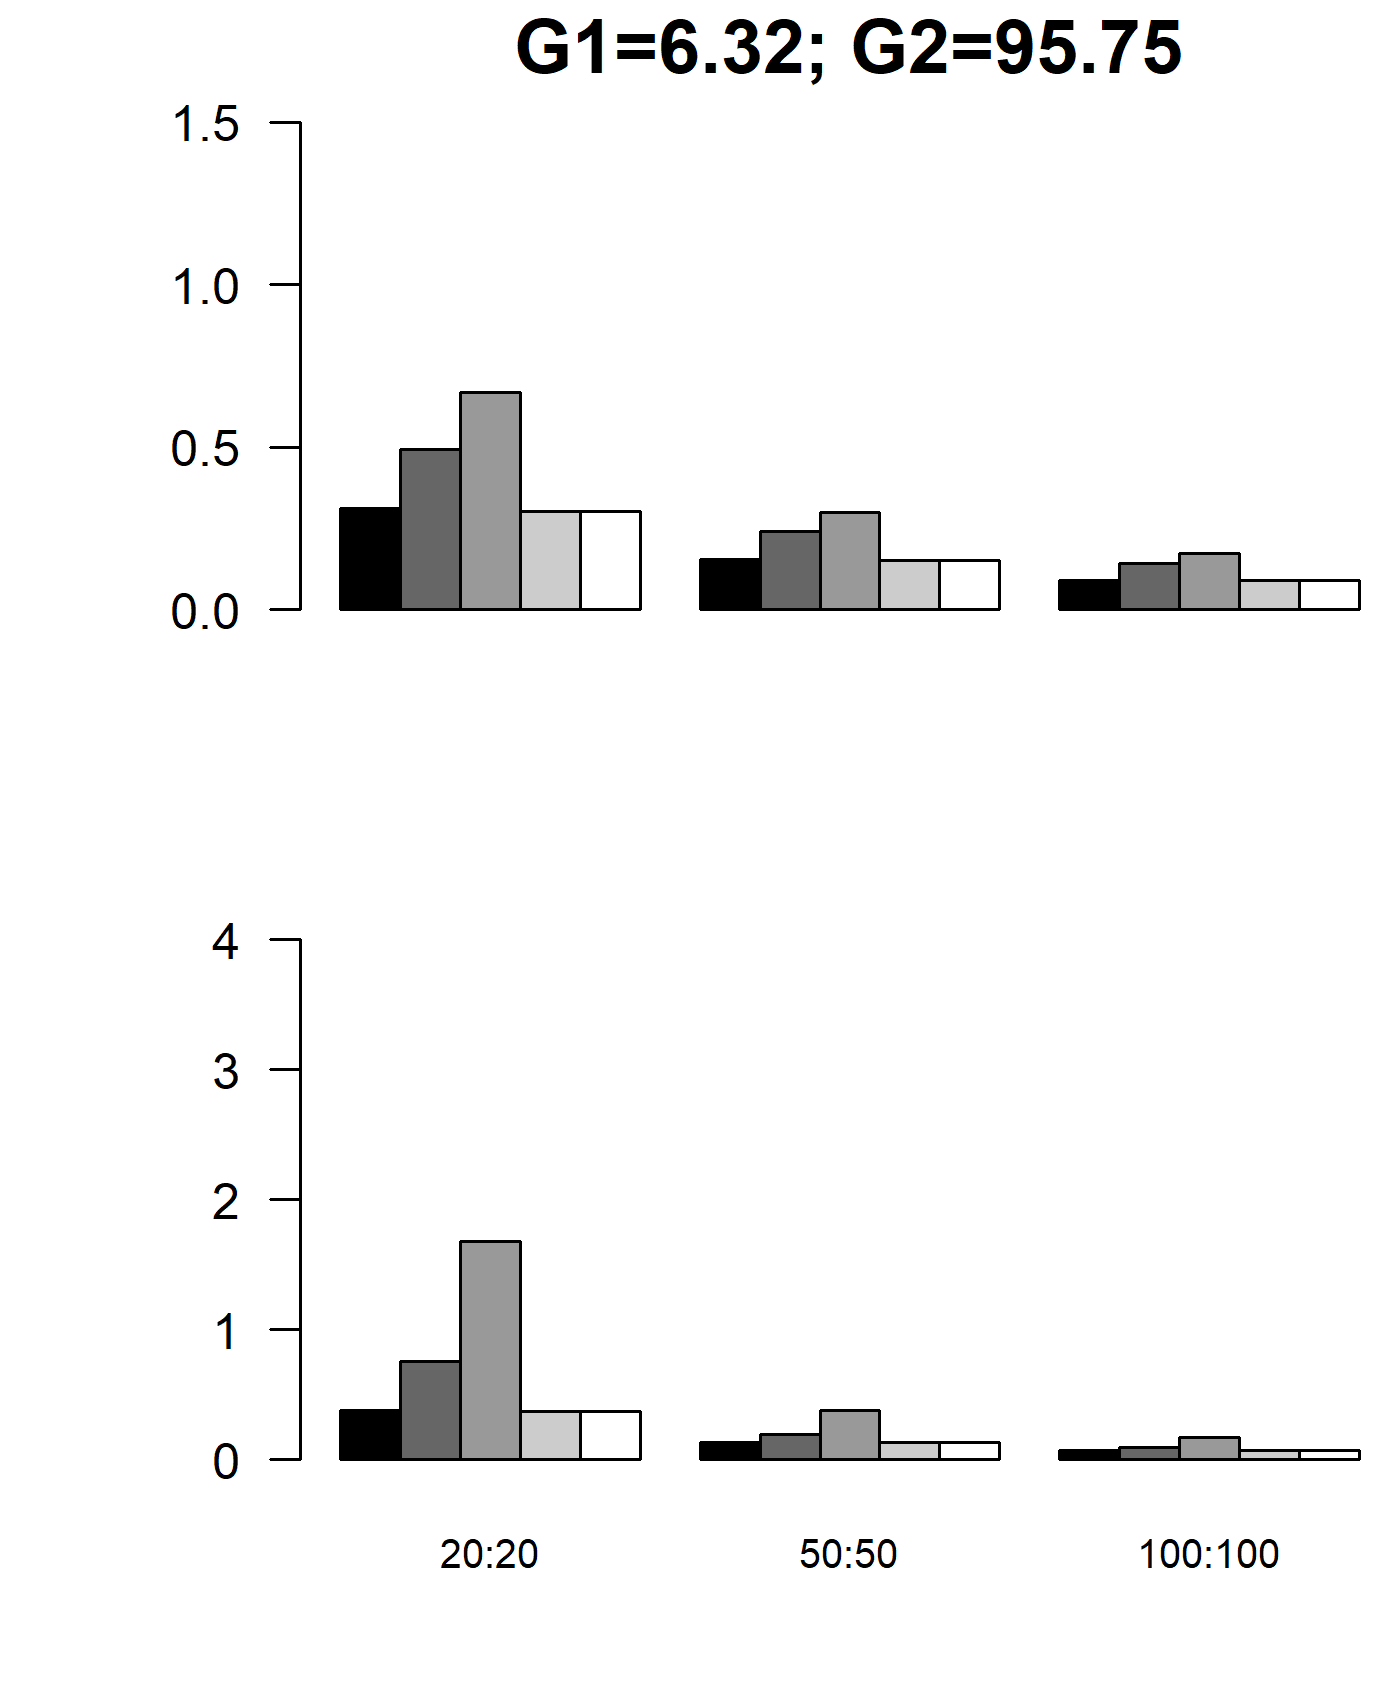
\includegraphics[width=0.2\linewidth]{C:/Users/Marie/Documents/Github_projects/Effect-sizes/Scripts outputs/Quality of ES measures/Graphs/id_Hom_bal/bias_eff,G1=6.32 & G2=95.75;id_Hom_bal} 

}

\caption{Bias and efficiency of estimators of standardized mean difference, when variances and sample sizes are equal across groups (condition a)}\label{fig:idHombal}
\end{sidewaysfigure}

\begin{sidewaysfigure}

{\centering 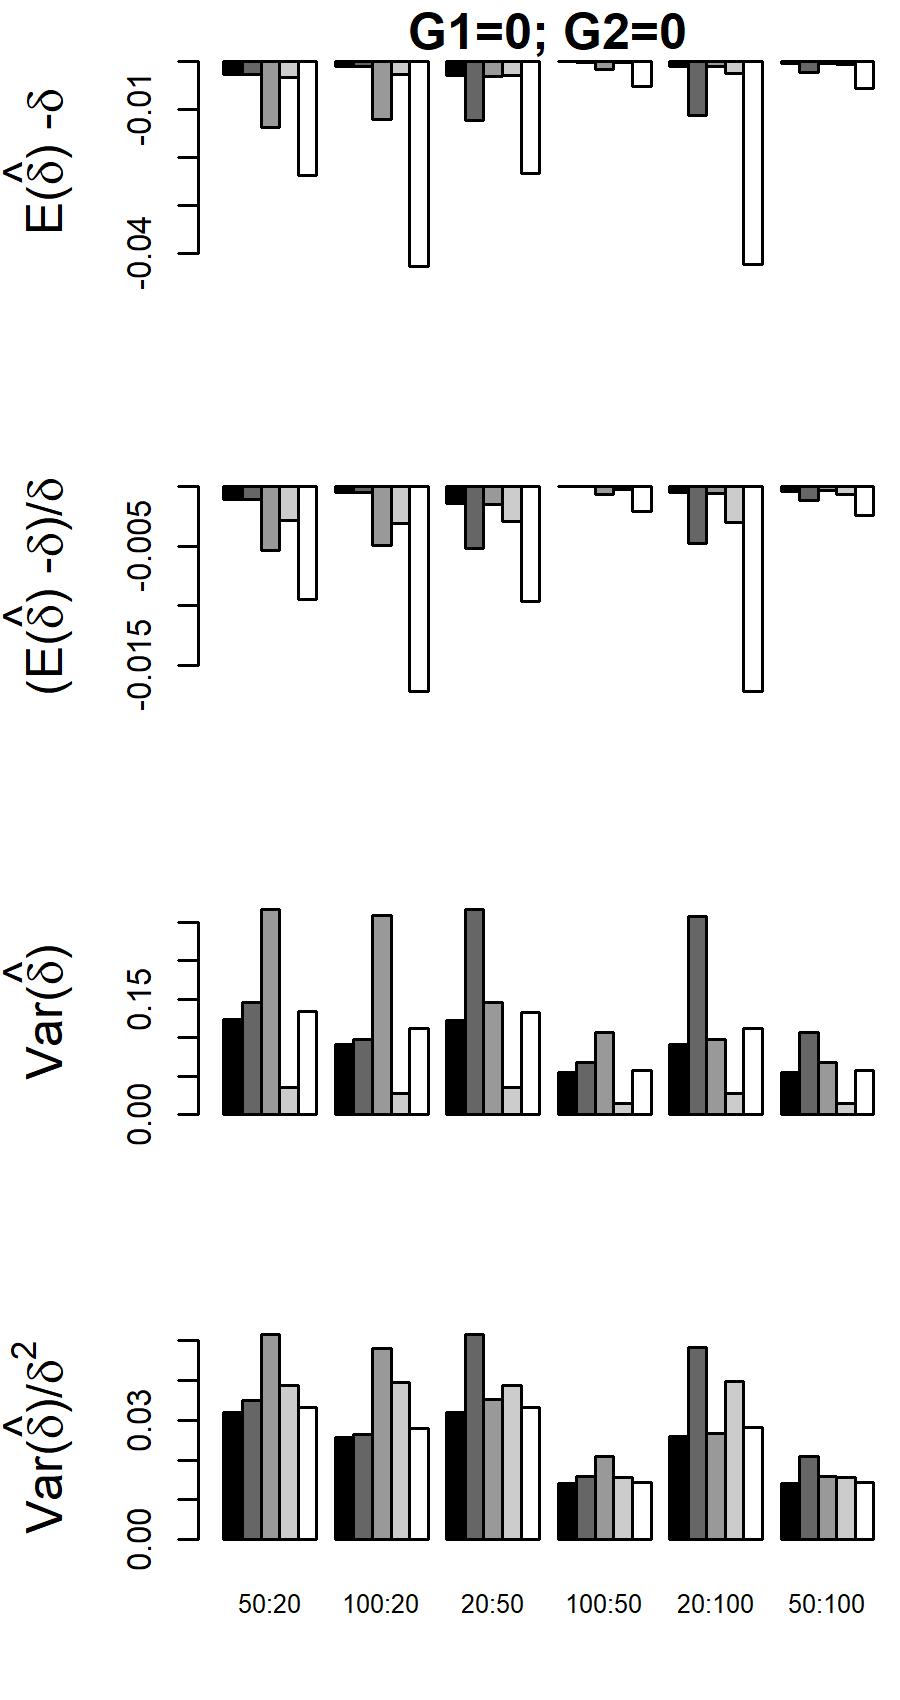
\includegraphics[width=0.2\linewidth]{C:/Users/Marie/Documents/Github_projects/Effect-sizes/Scripts outputs/Quality of ES measures/Graphs/id_Hom_rnull/bias_eff,G1=0 & G2=0;id_Hom_rnull} 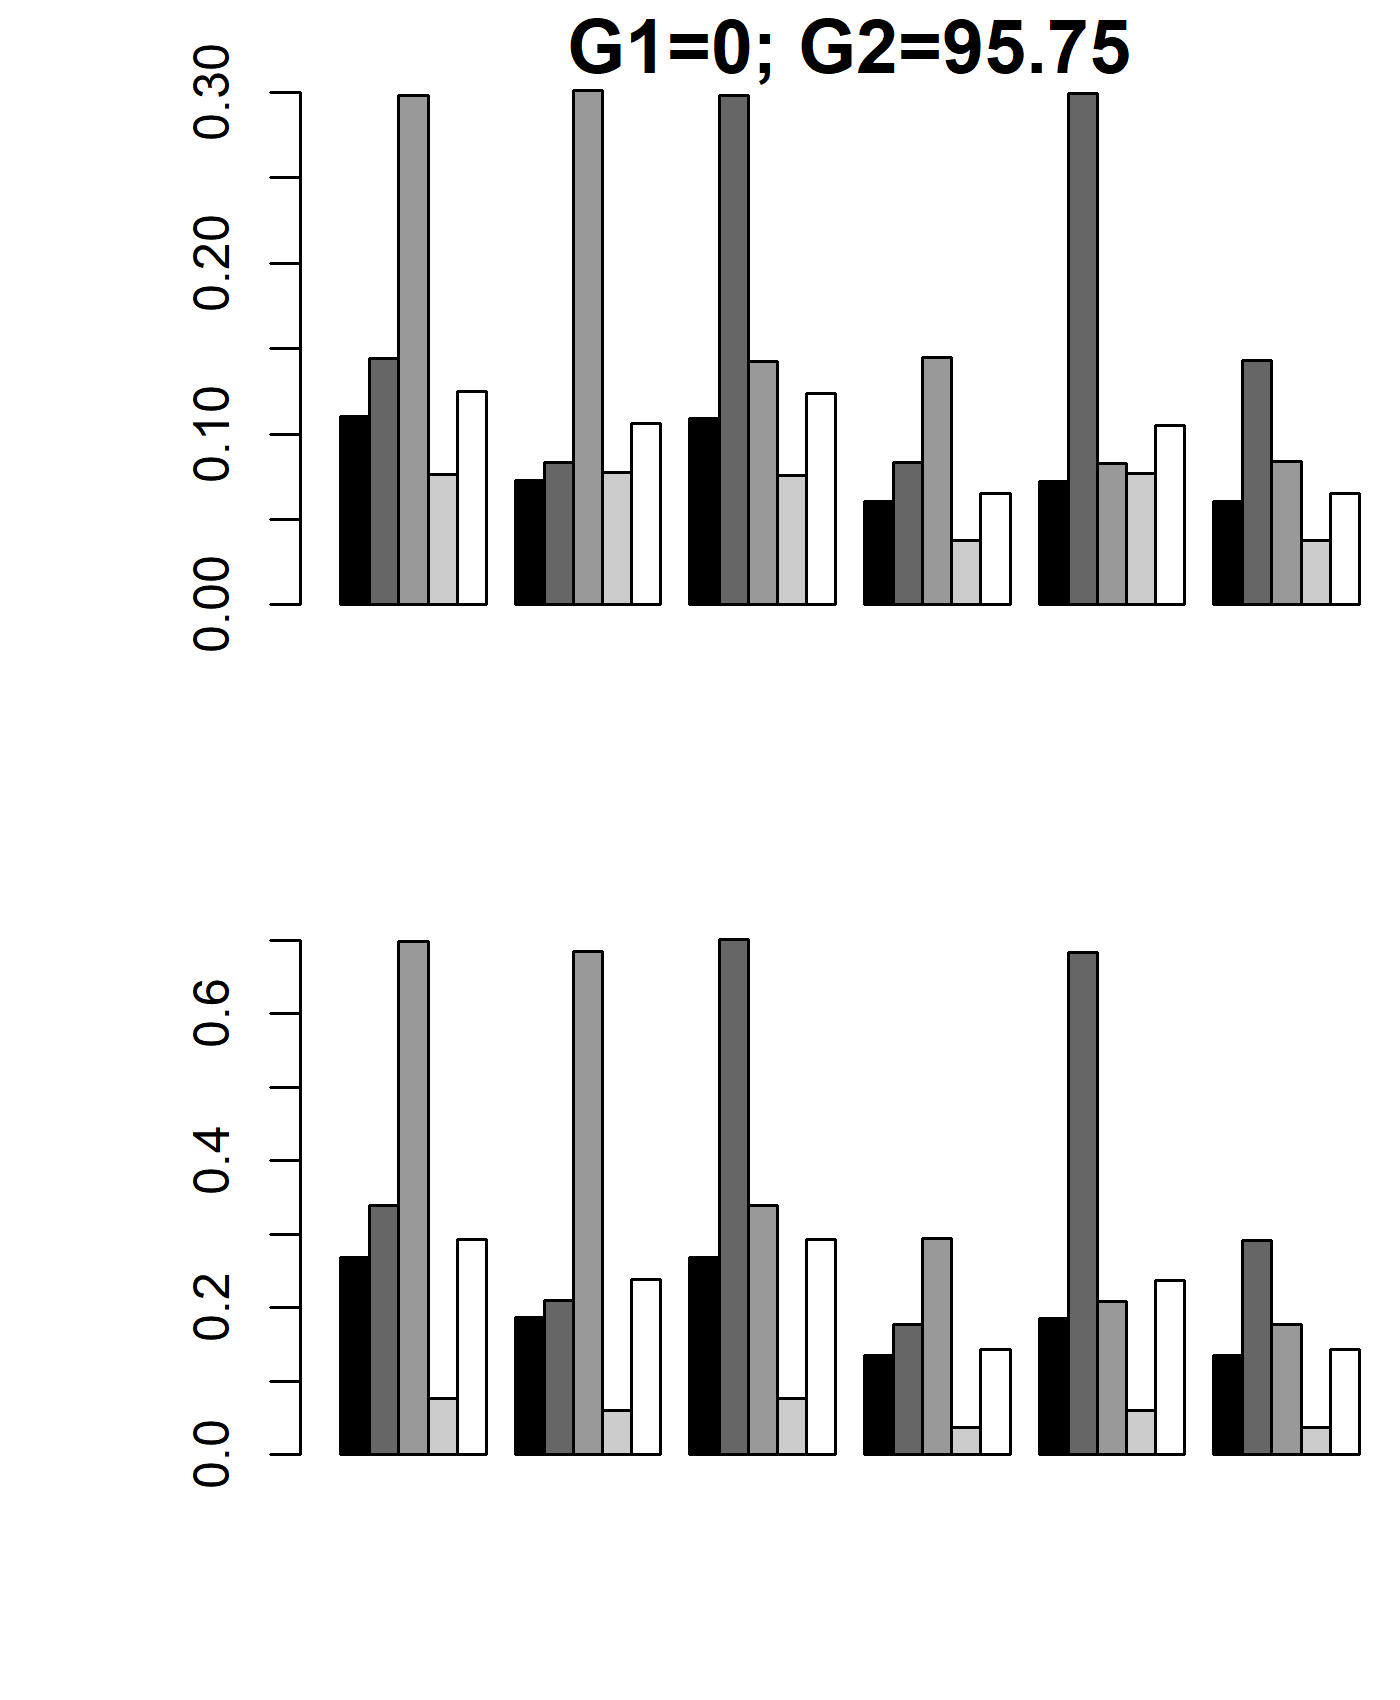
\includegraphics[width=0.2\linewidth]{C:/Users/Marie/Documents/Github_projects/Effect-sizes/Scripts outputs/Quality of ES measures/Graphs/id_Hom_rnull/bias_eff,G1=0 & G2=95.75;id_Hom_rnull} 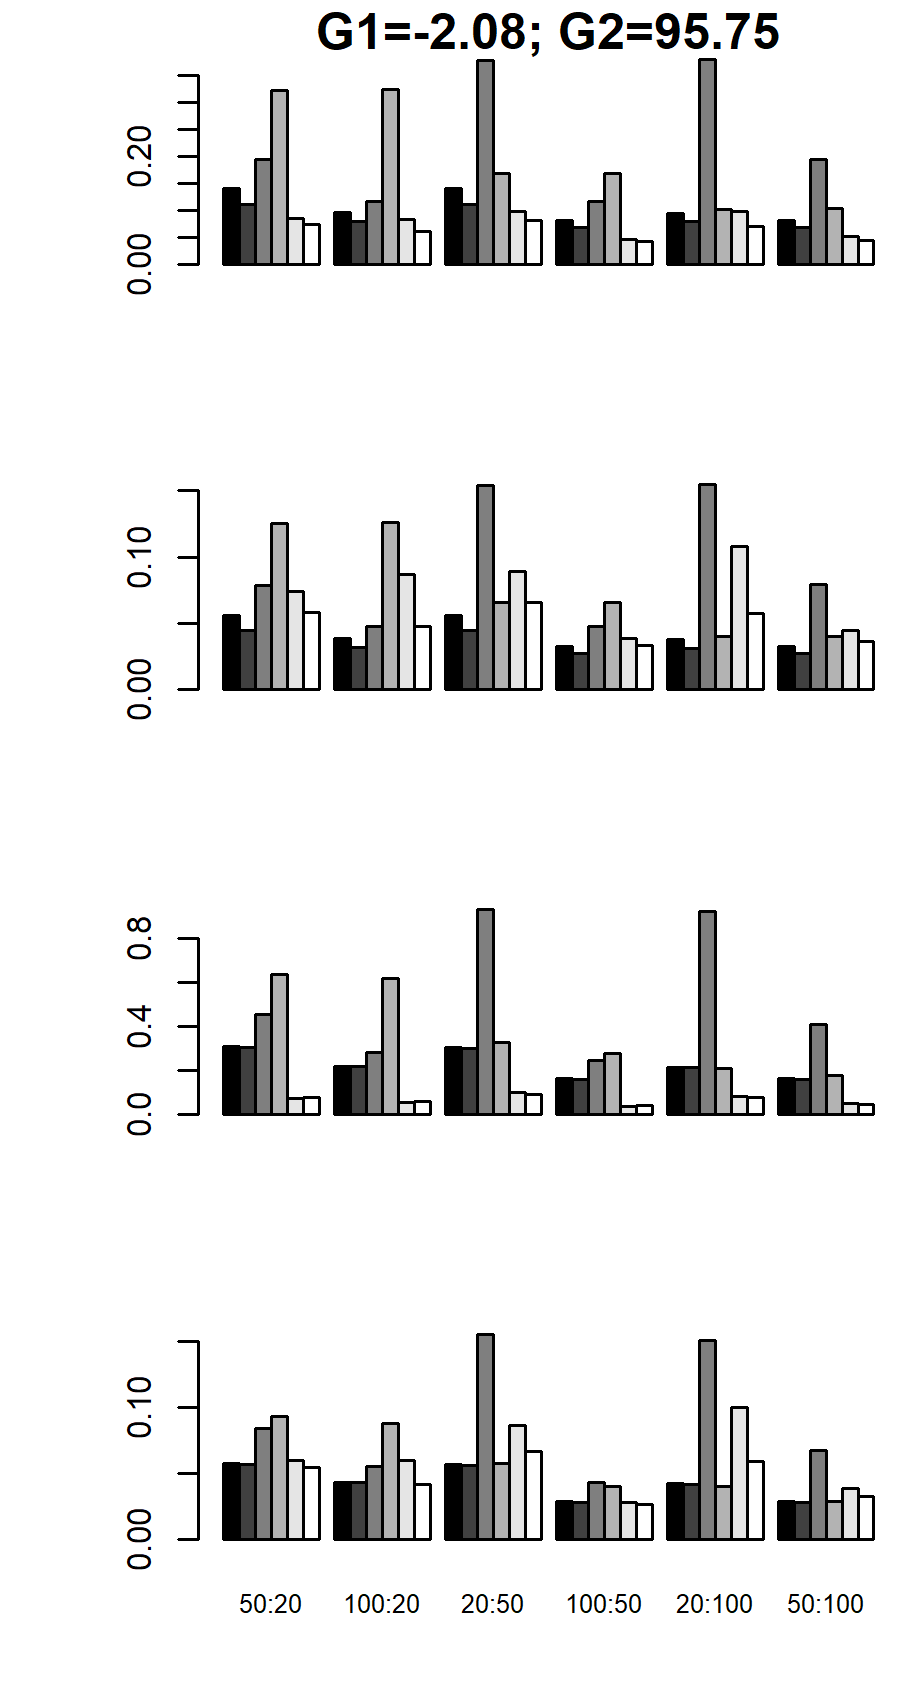
\includegraphics[width=0.2\linewidth]{C:/Users/Marie/Documents/Github_projects/Effect-sizes/Scripts outputs/Quality of ES measures/Graphs/id_Hom_rnull/bias_eff,G1=2.08 & G2=95.75;id_Hom_rnull} 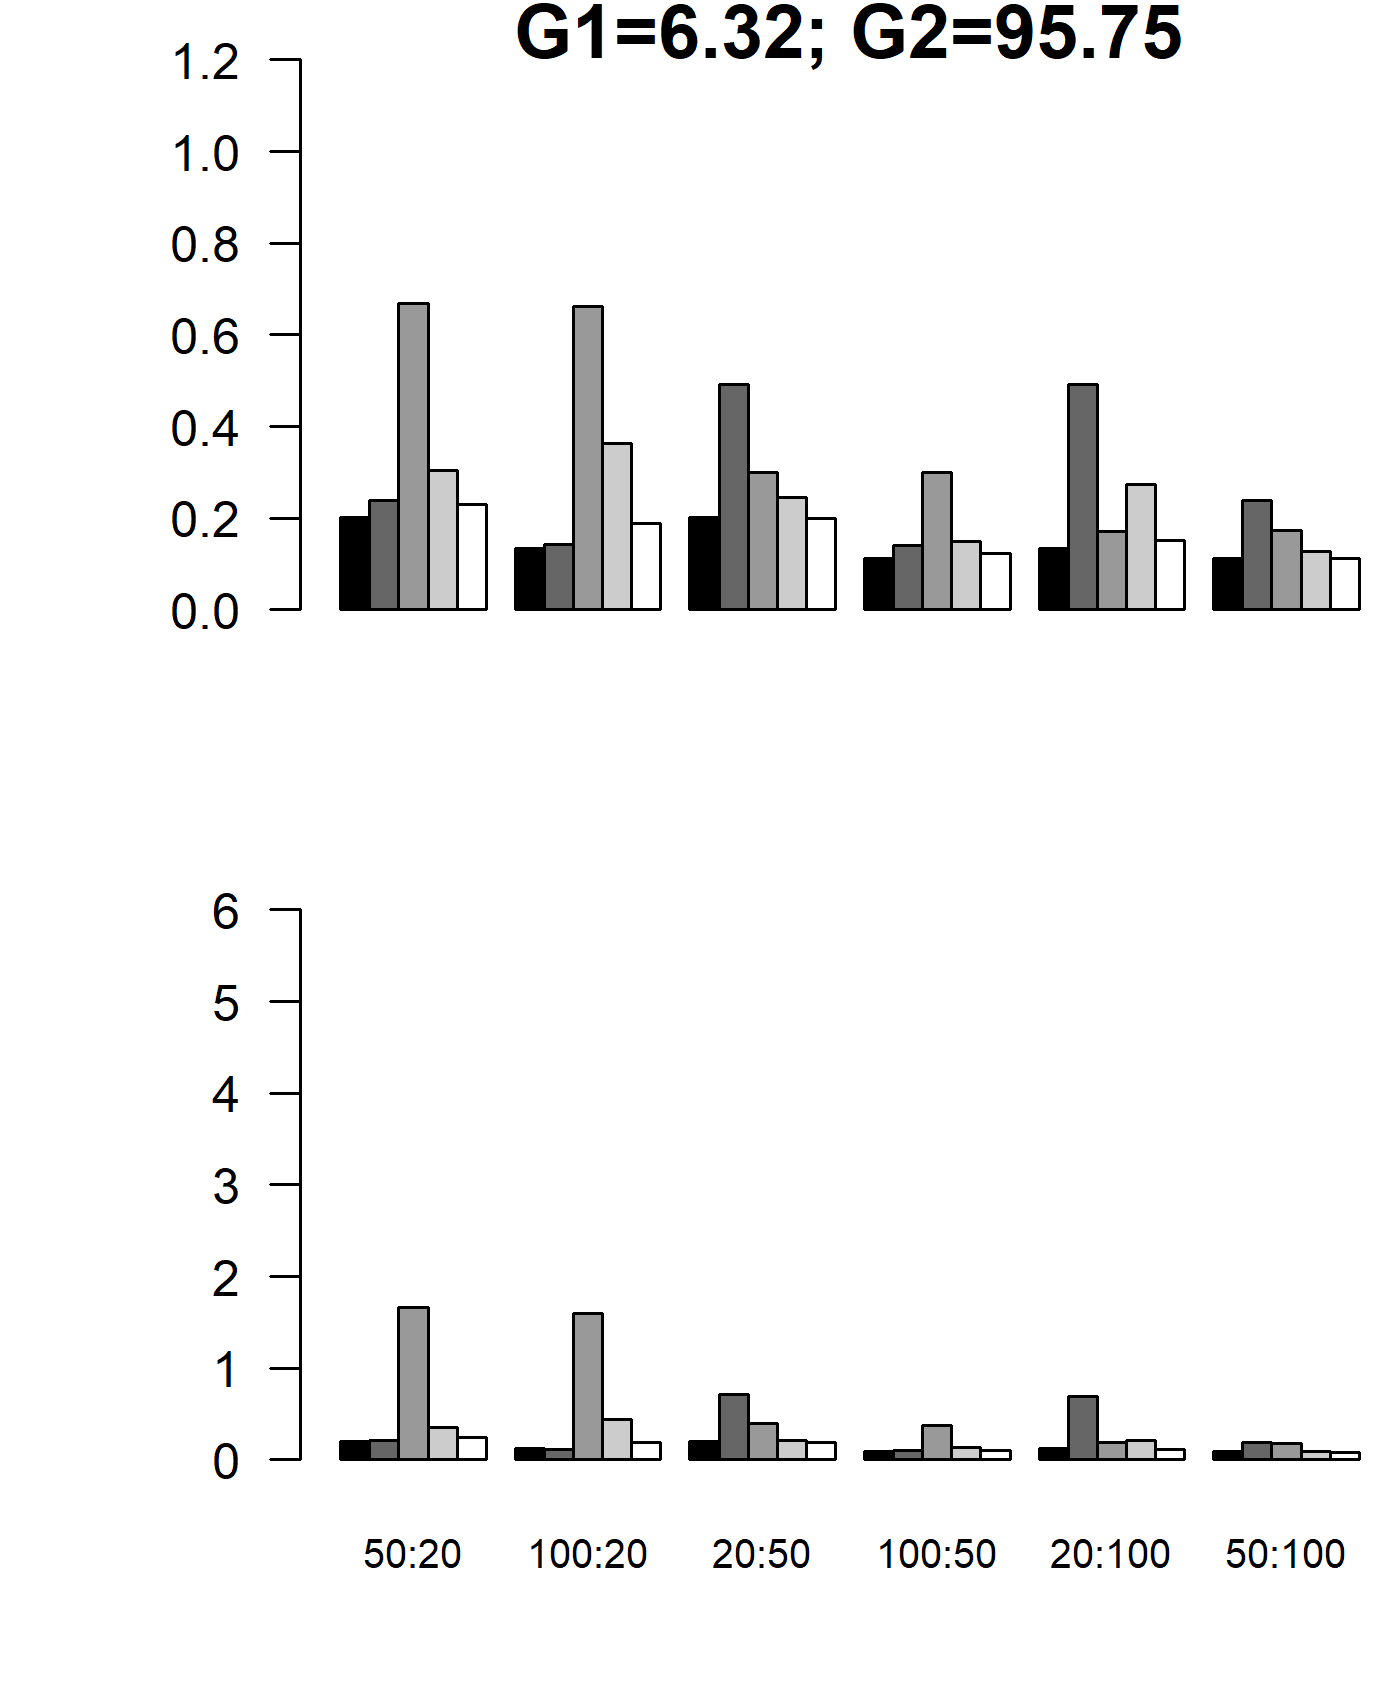
\includegraphics[width=0.2\linewidth]{C:/Users/Marie/Documents/Github_projects/Effect-sizes/Scripts outputs/Quality of ES measures/Graphs/id_Hom_rnull/bias_eff,G1=6.32 & G2=95.75;id_Hom_rnull} 

}

\caption{Bias and efficiency of estimators of standardized mean difference, when variances are equal across groups and sample sizes are unequal (condition b)}\label{fig:idHomrnull}
\end{sidewaysfigure}

Figures \ref{fig:idHombal} and \ref{fig:idHomrnull} represent configurations where the equality of variances assumption is met. Figure \ref{fig:idHombal} shows that when sample sizes are equal between groups (condition a), bias tends to decrease and precision is also improved with increasing sample sizes for all estimators, meaning that they are all consistent. Shieh's \(d_s\) and Shieh's \(d^*_s\) are identical, because our transformation is operant only when the sample sizes ratio differs from 1. We already knew from equations \ref{eq:biascohenshieh}, \ref{eq:varcohenshieh} and \ref{eq:cohenshieh} that when both assumptions of normality and equality of variances are met, the relative bias and variance of Cohen's \(d_s\) and Shieh's \(d_s\) are identical. Columns 2 to 4 in Figure \ref{fig:idHombal} reveal that this remains true for any departures from the normality assumptions. In accordance with our theoretical expectations, under samples are extracted from normal distributions (first column in in Figure \ref{fig:idHombal}), Hedge's \(g_s\) is less biased and slighly less variable than Cohen's \(d_s\). Columns 2 to 4 in Figure \ref{fig:idHombal} reveal that this remains true when samples are extracted from non normal distributions, even if the further from the normal distribution, the lower the difference between both estimators.

Both glass's \(d_s\) estimates (i.e.~using \(SD_1\) and \(SD_2\)) show least precision and highest bias rates, in comparison with all other measures. When samples are extracted from symmetric ditributions (the two first columns in Figure \ref{fig:idHombal}), Glass's \(d_s\) shows similar performances when using either \(SD_1\) or \(SD_2\) as standardizer. On the other side, when samples are extracted from skewed distributions, it shows unequal performances as a function of the chosen standardizer, because there is a non null correlation between the sample means and sample standard deviations, resulting in a non null correlation of opposite sign between \(\bar{X_1}-\bar{X_2}\) and respectively \(SD_1\) and \(SD_2\).\footnote{When distributions are right-skewed, the correlation between sample means and standard deviation is positive. Because SD1 (SD2) is positively (negatively) correlated with the mean difference estimates, it results in a positive (negative) correlation between SD1 (SD2) and the mean difference. when distributions are left-skewed, the correlation between sample means and standard deviation is negative. Because SD1 (SD2) is positively (negatively) correlated with the mean difference estimates, it results in a negative (positive) correlation between SD1 (SD2) and the mean difference.  When the population mean difference $\mu_1-\mu_2$ is positive (like in our simulations), Glass's $d_s$ is always more biased and variable when choosing as standardizer the $SD$ that is negatively correlated with $\bar{X_1}-\bar{X_2}$ (i.e. $SD_2$ when distributions are right-skewed and $SD_1$ when distributions are left-skewed). When the population mean difference is negative, the reverse is true. For interested reader, this is detailed and explained in Appendix 3.}.

Figure \ref{fig:idHomrnull} shows that when sample sizes are unequal between groups, Glass's \(d_s\) and Shieh's \(d_s\) are sometimes unconsistent, meaning that their bias and variance will remain identical or even increase when the total sample size increases. We know from Table 1 that under the assumptions of normality, the bias of Glass's \(d_s\) does not depend either on the size of the experimental group or on the total sample size. Our simulations reveal that it remains true for any departures from the normality assumption. The only way to decrease the bias of Glass's \(d_s\) is therefore to add subjects in the control group. One can see, for example, that when there are 50 subjects in the control group, the bias will remain identical when there are respectively 20 and 100 subjects in the experimental group. On the other side, the variance of Glass's \(d_s\) depends on the sample size of both control and experimental groups, however, Glass's \(d_s\) will be less variable when there are more subjects in the control group than when there are more subjects in the experimental group {[}A NOTER QU UN TROP GRAND NRATIO N EST PAS BON NON PLUS\ldots{} VOIR FICHIER REFLEXION TEST1 ET TEST2\ldots{]}. Finally, as previously observed in Figure \ref{fig:idHombal}, the bias and variances of Glass's estimates also depends on the correlation between \(\bar{X_1}-\bar{X_2}\) and the standardizer, when distribution are skewed. In our simulations, the worst configuration will occure when the standardizer is computed with the smaller group and is negatively correlated with the sample means difference (i.e.~when choosing SD2 when distributions are right-skewed, and when choosing SD1 when distributions are left-skewed).\footnote{Again, we should remind that in all our simulations, the population mean difference is positive. If mean difference were negative, glass's $d_s$ would be more biased and variable when the chosen standardizer is positively correlated with the mean difference and associated with the smaller sample size.}

Increasing sample size will decrease the bias and variance of Shieh's \(d_s\) only when the sample sizes ratio remains close to 1. For example, one can observe that when there are 100 subjects in the first group, the bias and variance of Shieh's \(d_s\) are smaller when there are 50 subjects in the second group than when there are only 20 subjects, because the sample size ratio decreases. On the other side, when there are 20 subjects in the first group, the bias and variance of Shieh's \(d_s\) are larger when there are 100 subjects in the second group than when there are only 50 subjects in the second group, because despite the increasing total sample size, the sample size ratio increases.{[}REGARDER AVEC CHRISTOPHE LES GRAPHIQUES, DC MON DOC DE REFLEXION: Quest-ce qui compte le plus? le N ou le NRATIO? Au départ, ajouter du N diminue le biais mais assez vite, la tendance s'inverse. Nuance nécessaire à préciser?{]}

Our transformed Shieh's \(d^*_s\) is always less biased and variable than Shieh's \(d_s\). Moreover, unlike Shieh's \(d_s\), Shieh's \(d^*_s\) is consistent, meaning that for any sample size ratio, the bias and variance will decrease with increasing sample size. Raw bias and variance of Shieh's \(d_s^*\) appear to be smaller than the bias and variance of Cohen's \(d_s\), however, this is only due to the fact that Shieh's \(d_s^*\) is always smaller than Cohen's \(d_s\) (see Appendix 1 for the relation between both estimators). When looking at the second and fourth rows in Figure \ref{fig:idHomrnull}, we can see that the relative bias and variance of Shieh's \(d^*_s\) are larger than the relative bias and variance of Cohen's \(d_s\), that remains a better indicator. Finally, Hedge's \(g_s\) is always less biased and slighly less variable than Cohen's \(d_s\), especially when samples are extracted from normal distributions.

In conclusion, Glass's \(d_s\) should always be avoided when the equality of variance assumption is met. Cohen's \(d_s\) and Shieh's \(d_s\) are equally performant as long as the sample size ratio is close to 1. However, when designs are highly unbalanced, Shieh's \(d_s\) is not consistent anymore. While Shieh's \(d^*_s\) corrects this inconsistency, Cohen's \(d_s\) remains a better estimator. Finally, whatever designs are balanced or not, Hedge's correction reduce the relative bias of Cohen's \(d_s\) and is therefore the best estimator.

\hypertarget{when-variances-are-unequal-across-groups}{%
\subparagraph{When variances are unequal across groups}\label{when-variances-are-unequal-across-groups}}

\begin{sidewaysfigure}

{\centering 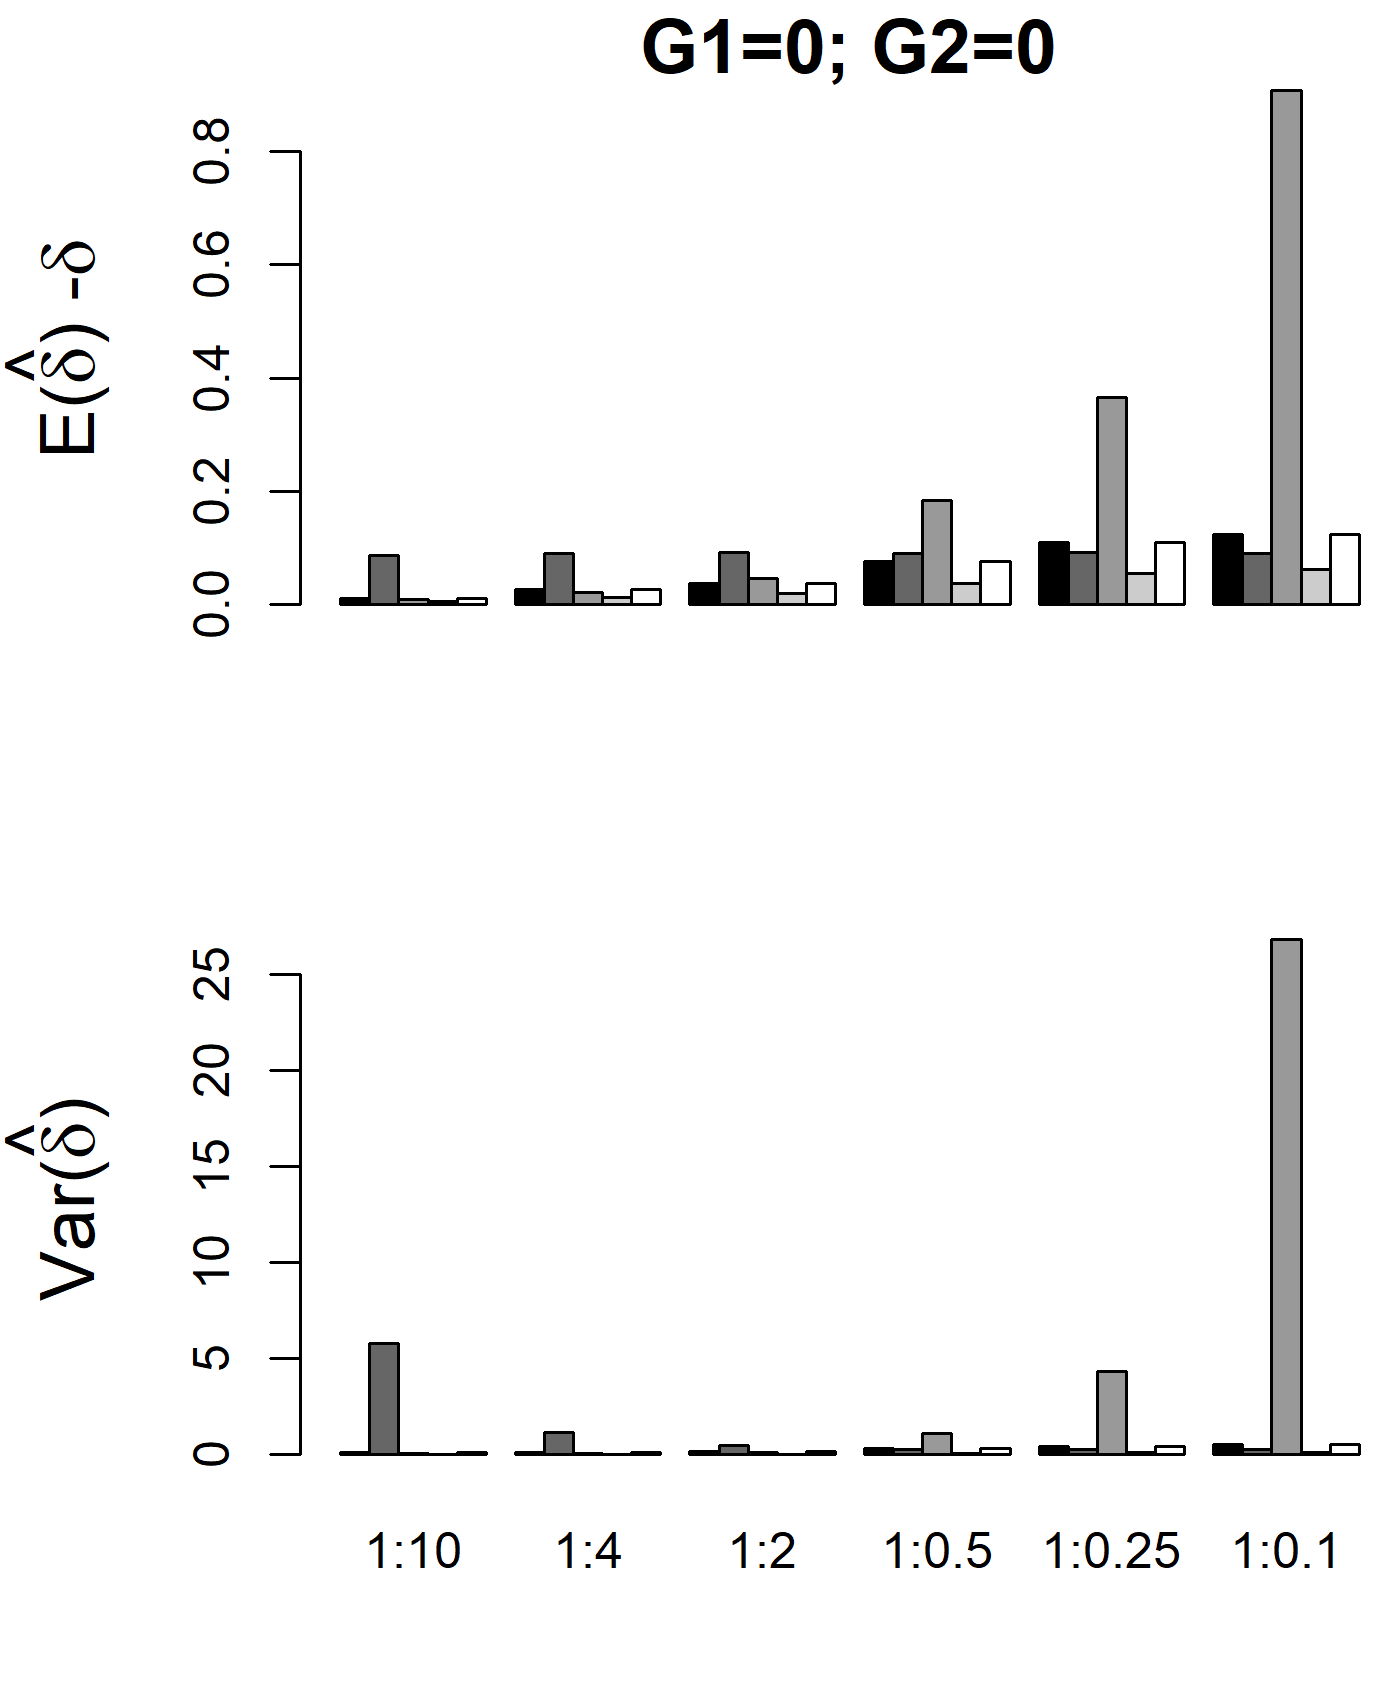
\includegraphics[width=0.2\linewidth]{C:/Users/Marie/Documents/Github_projects/Effect-sizes/Scripts outputs/Quality of ES measures/Graphs/id_Het_bal/bias_eff,G1=0 & G2=0;id_Het_bal} 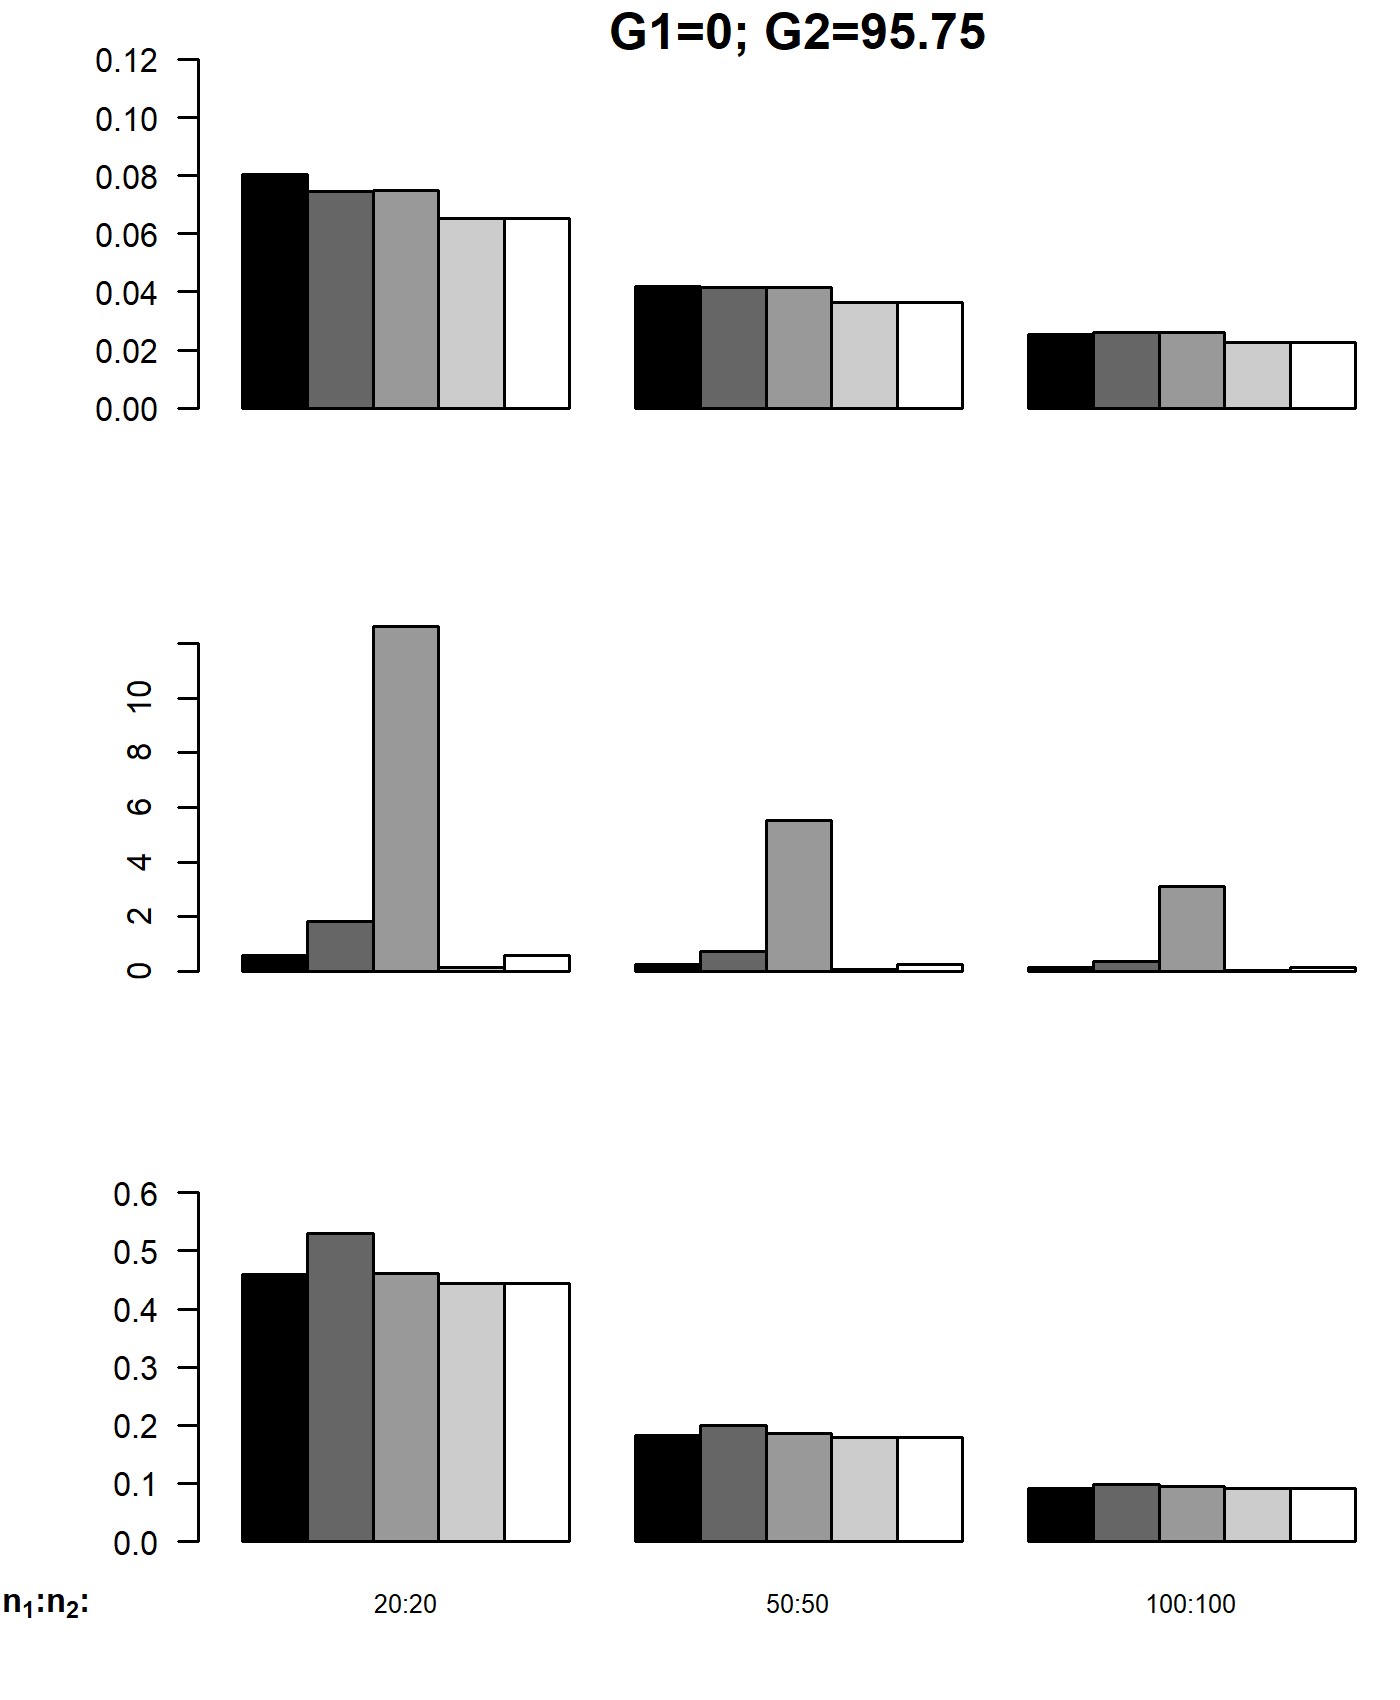
\includegraphics[width=0.2\linewidth]{C:/Users/Marie/Documents/Github_projects/Effect-sizes/Scripts outputs/Quality of ES measures/Graphs/id_Het_bal/bias_eff,G1=0 & G2=95.75;id_Het_bal} 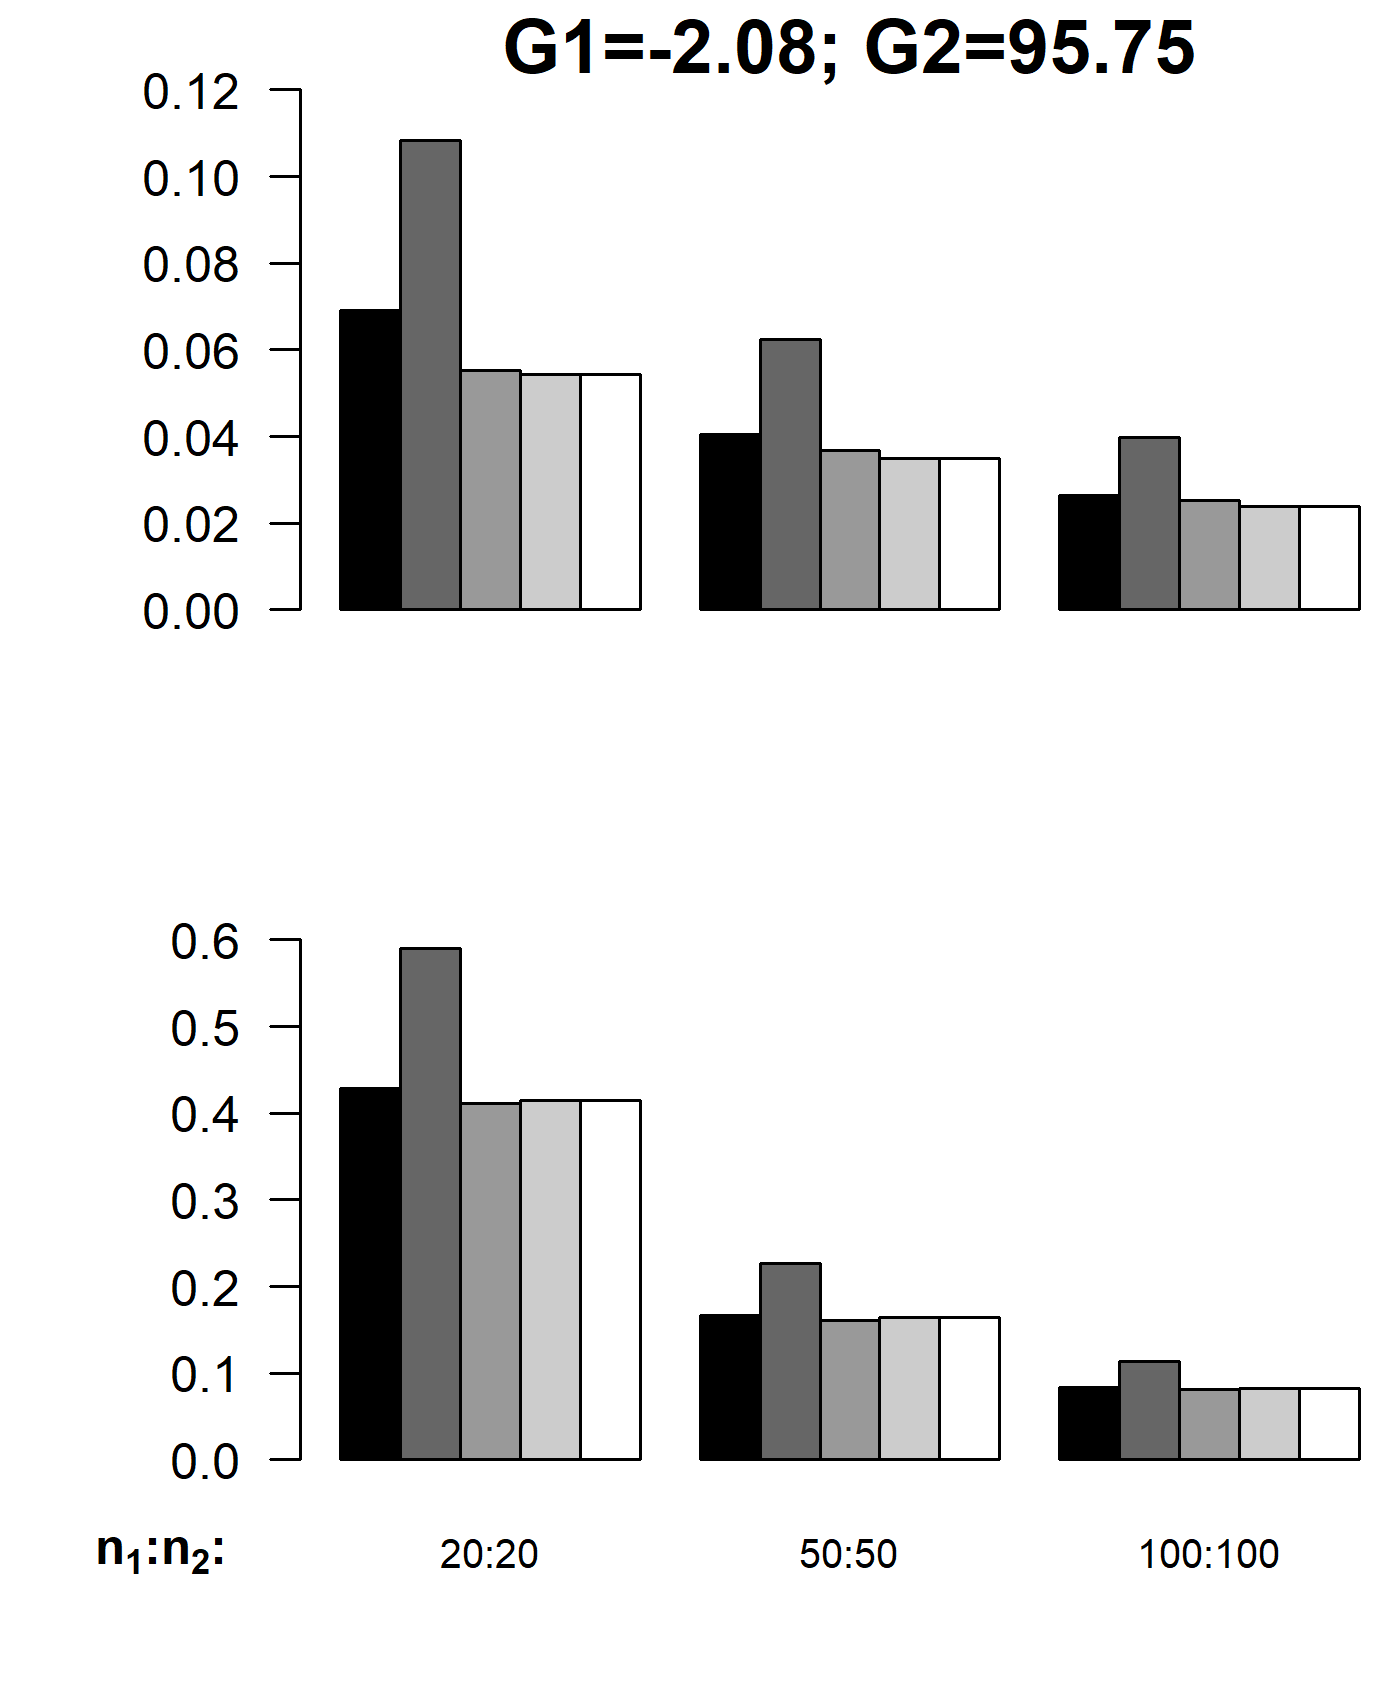
\includegraphics[width=0.2\linewidth]{C:/Users/Marie/Documents/Github_projects/Effect-sizes/Scripts outputs/Quality of ES measures/Graphs/id_Het_bal/bias_eff,G1=2.08 & G2=95.75;id_Het_bal} 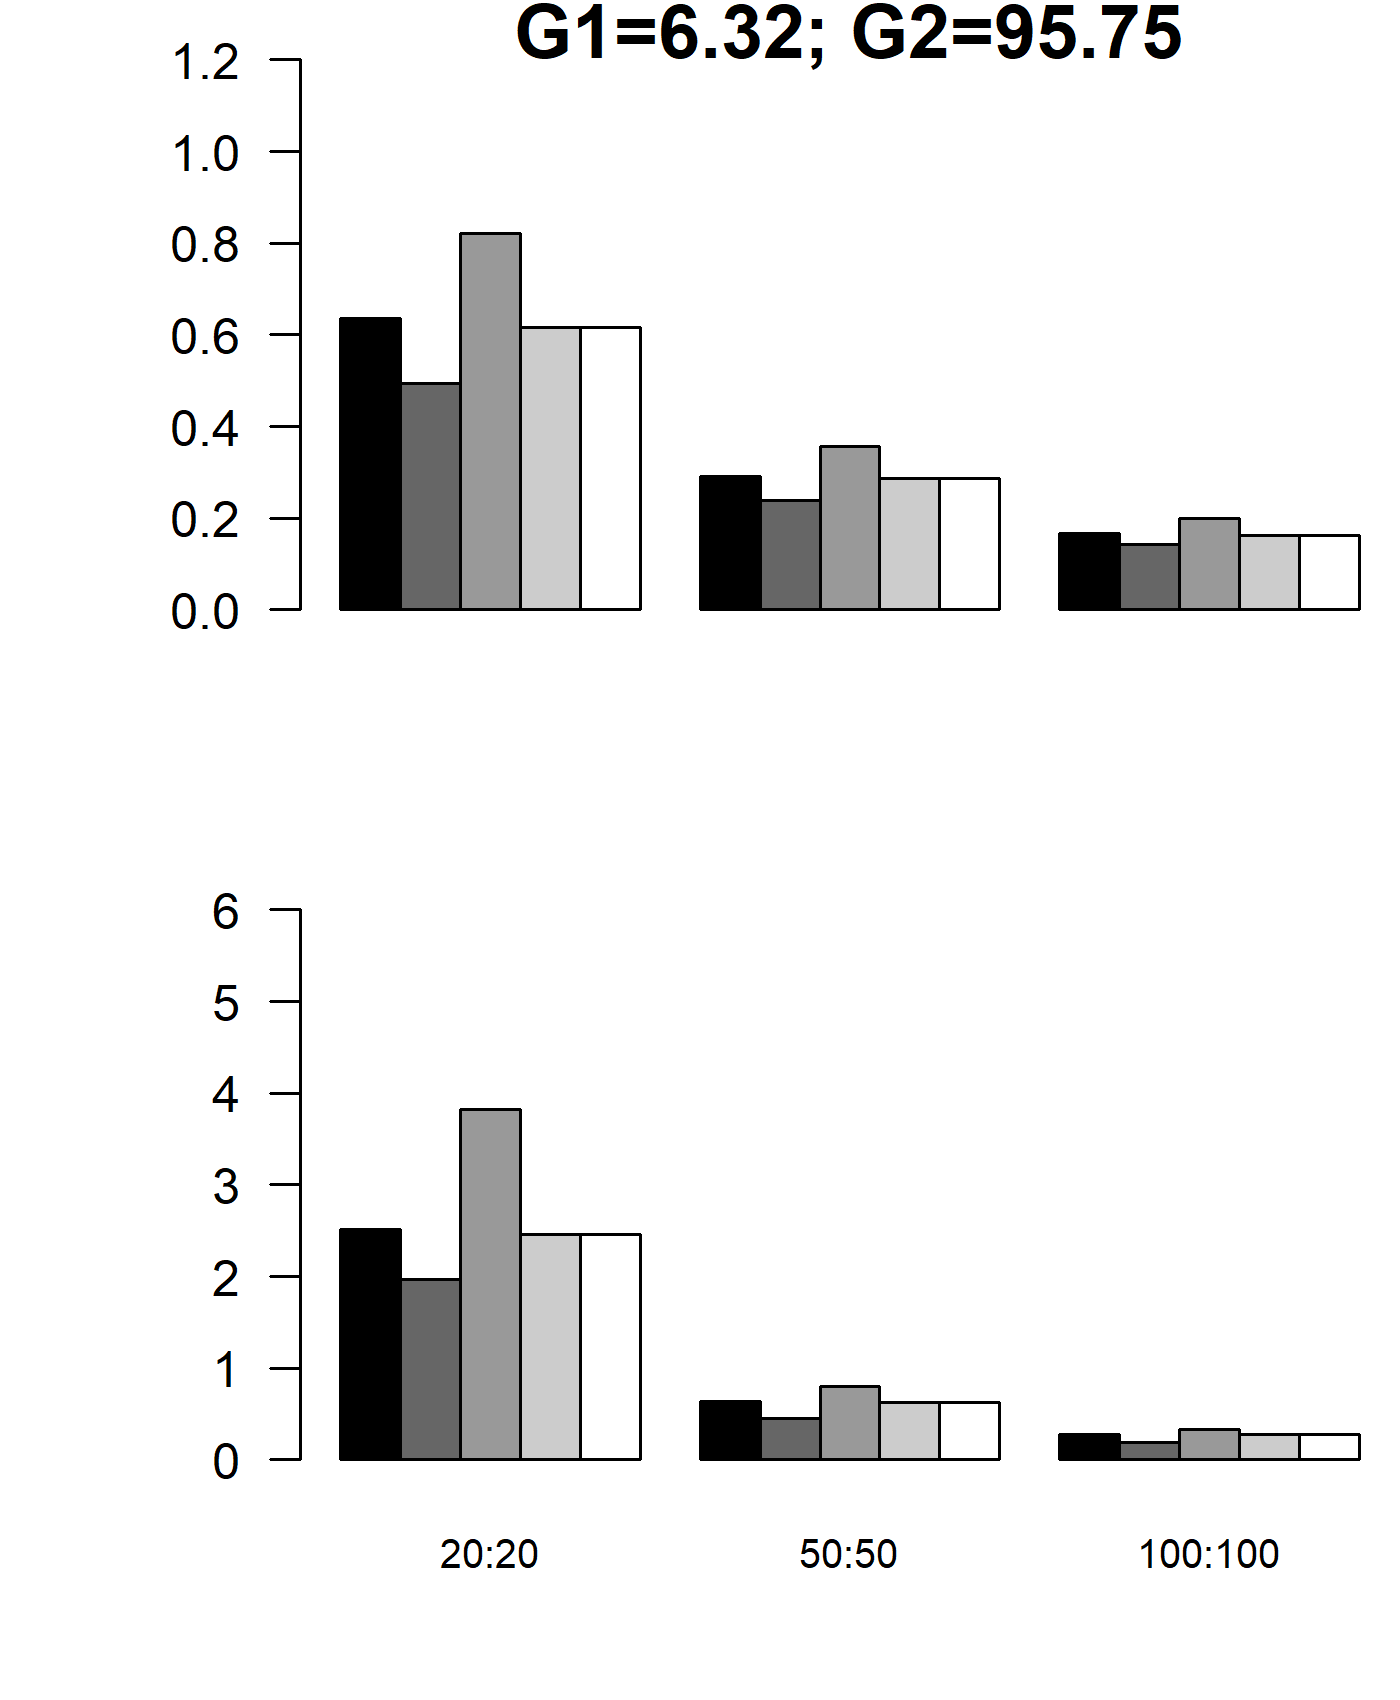
\includegraphics[width=0.2\linewidth]{C:/Users/Marie/Documents/Github_projects/Effect-sizes/Scripts outputs/Quality of ES measures/Graphs/id_Het_bal/bias_eff,G1=6.32 & G2=95.75;id_Het_bal} 

}

\caption{Bias and efficiency of estimators of standardized mean difference, when variances are unequal across groups and sample sizes are equal (condition c)}\label{fig:idHetbal}
\end{sidewaysfigure}

Figure \ref{fig:idHetbal} shows that all estimators are consistent, even when variances are unequal between groups, as long as sample sizes are equal across groups (condition c). Shieh's \(d_s\) and Shieh's \(d^*_s\) are identical, because our transformation is operant only when the sample sizes ratio differs from 1. Figure \ref{fig:idHombal} previously revealed that the relative performances of Cohen's \(d_s\) and Shieh's \(d_s\) remained identical for any departures from the normality assumption. Figure \ref{fig:idHetbal} now reveals that this remains unchanged when there is heteroscedasticity, meaning that anytime sample sizes are equal across groups, Cohen's \(d_s\) and Shieh's \(d_s\) are equally performant. As previously, Hedge's \(g_s\) is less biased and slighly more efficient (i.e.~less variable) than Cohen's \(d_s\), Shieh's \(d_s\) and Shieh's \(d^*_s\).

When the normality assumption is met, both Glass's estimators are more biased than all other estimators. When distributions are symmetric with heavy-tailed distributions, both Glass's estimators are more biased and variable than all other estimators. In terms of relative bias, Glass's \(d_s\) shows similar performances when using either \(SD_1\) or \(SD_2\) as standardizer\footnote{When looking at the raw bias in Figure 4, one could believe that the bias is always more important when choosing SD2 as a standardizer. It is only an artefact of simulations. The bias is always more important when choosing the sample extracted from the smaller population SD as standardiser, because it results in a larger effect size estimate, and the larger the effect size estimate, the larger the raw bias. In our simulations, while the population SD of the first group always equals 1, in half of the simulations in condition c, the population SD of the second group is lower than 1 (meaning that the more biased Glass's estimate will occure when choosing SD2 < 1 as standardiser), and in the other half, the population SD of the second group is larger than 1 (meaning that the more biased Glass's estimate will occure when choosing SD1 as standardizer). Of course, for X, a constant mean difference and z, the standardizer, X/z will always result in a larger effect size measure when z < 1. This is confirmed by the identical average relative bias for both measures of Glass's ds.}. However, the relative variances is larger when computing the standardizer based on the sample extracted from the less variable population, as shown in Figures \ref{fig:idHetbal2} and \ref{fig:idHetbal3}. {[}POURQUOI PAS VRAI QD DISTRIBUTIONS NORMALES ALORS QUE D APRES LA FORMULE DE LA VARIANCE DU GLASS CA DEVRAIT ETRE LE CAS TT LE TPS?{]}.

When samples are extracted from skewed distributions, as previously, Glass's \(d_s\) using either \(SD_1\) or \(SD_2\) as standardizer show unequal performances, due to correlations of opposite sign between \(\bar{X_1}-\bar{X_2}\) and respectively \(SD_1\) and \(SD_2\). While Glass's \(d_s\) estimates were always less performant than all other estimators when variances were equal across groups, these are sometimes more biased and variable, and sometimes less biased and variable than all other estimators when population variances are unequal across groups. The explanation also lies in the correlation between \(\bar{X_1}-\bar{X_2}\) and standardizers: as long as population variances are equal across groups, standardizers taking both \(SD_1\) and \(SD_2\) into account are uncorrelated with \(\bar{X_1}-\bar{X_2}\). However, when population variances are unequal across groups, the sign of the correlation between the standardizer and the mean difference will be the same as the one of the correlation between the mean difference and the estimates of the larger population variance, as summarized in Table 4. It explains why Glass's \(d_s\) is sometimes more, sometimes less performant than other estimators. {[}EXCEPTION: BIAIS RELATIF QUAND SD1\textgreater SD2? ET DISTRIBUTIONS ARE LEFT-SKEWED. Marche dans tous les autres cas.{]}

\newpage

Table 4.
\emph{Correlation between standardizers (\(SD_1\),\(SD_2\) and others) and \(\bar{X_1}-\bar{X_1}\), when samples are extracted from skewed distributions with unequal variances, as a function of the SD-ratio}

\begin{longtable}[]{@{}lcc@{}}
\toprule
& \textbf{\textbf{population distribution}} &\tabularnewline
\midrule
\endhead
& \emph{right-skewed} & \emph{left-skewed}\tabularnewline
& --------------------------- & ---------------------------\tabularnewline
When \(\sigma_1=\sigma_2\) & \(SD_1\): \emph{positive} & \(SD_1\): \emph{negative}\tabularnewline
& \(SD_2\): \emph{negative} & \(SD_2\): \emph{positive}\tabularnewline
& Others: \emph{null} & Others: \emph{null}\tabularnewline
& &\tabularnewline
When \(\sigma_1>\sigma_2\) & \(SD_1\): \emph{positive} & \(SD_1\): \emph{negative}\tabularnewline
& \(SD_2\): \emph{negative} & \(SD_2\): \emph{positive}\tabularnewline
& Others: \emph{positive} & Others: \emph{negative}\tabularnewline
& &\tabularnewline
When \(\sigma_1<\sigma_2\) & \(SD_1\): \emph{positive} & \(SD_1\): \emph{negative}\tabularnewline
& \(SD_2\): \emph{negative} & \(SD_2\): \emph{positive}\tabularnewline
& Others: \emph{negative} & Others: \emph{positive}\tabularnewline
& &\tabularnewline
\bottomrule
\end{longtable}

\emph{Note.} When the population mean difference \(\mu_1-\mu_2\) is positive, like in our simulations, estimators are less performant when the correlation between standardizer and \(\bar{X_1}-\bar{X_2}\) is negative. Moreover, for equal sign of correlation, estimator using both \(SD_1\) and \(SD_2\) in the standardizer computation will always be more performant than estimator using the estimate of only one population variance as standardizer. For example, when samples are extracted from right-skewed distributions with \(\sigma_1 < \sigma_2\), glass's \(d_s\) using \(SD_1\) as standardizer will be the less variable estimator, because \(SD_1\) is positively correlated with \(\bar{X_1}-\bar{X_2}\).Glass's \(d_s\) using \(SD_2\) as standardizer will be the more variable estimator, because \(SD_2\) is negatively correlated with \(\bar{X_1}-\bar{X_2}\), as well as all other estimators using both \(SD_1\) and \(SD_2\) in the standardizer computation.

\begin{sidewaysfigure}

{\centering \includegraphics[width=0.2\linewidth]{C:/Users/Marie/Documents/Github_projects/Effect-sizes/Scripts outputs/Quality of ES measures/Graphs/subconditions/hetBal/bias_eff,G1=0 & G2=0;id_SDsd_bal2} \includegraphics[width=0.2\linewidth]{C:/Users/Marie/Documents/Github_projects/Effect-sizes/Scripts outputs/Quality of ES measures/Graphs/subconditions/hetBal/bias_eff,G1=0 & G2=95.75;id_SDsd_bal2} \includegraphics[width=0.2\linewidth]{C:/Users/Marie/Documents/Github_projects/Effect-sizes/Scripts outputs/Quality of ES measures/Graphs/subconditions/hetBal/bias_eff,G1=2.08 & G2=95.75;id_SDsd_bal2} \includegraphics[width=0.2\linewidth]{C:/Users/Marie/Documents/Github_projects/Effect-sizes/Scripts outputs/Quality of ES measures/Graphs/subconditions/hetBal/bias_eff,G1=6.32 & G2=95.75;id_SDsd_bal2} 

}

\caption{Bias and efficiency of estimators, when sample sizes are equal across groups and population variances are unequal, when SD1 is larger than SD2 (condition c1)}\label{fig:idHetbal2}
\end{sidewaysfigure}

\begin{sidewaysfigure}

{\centering 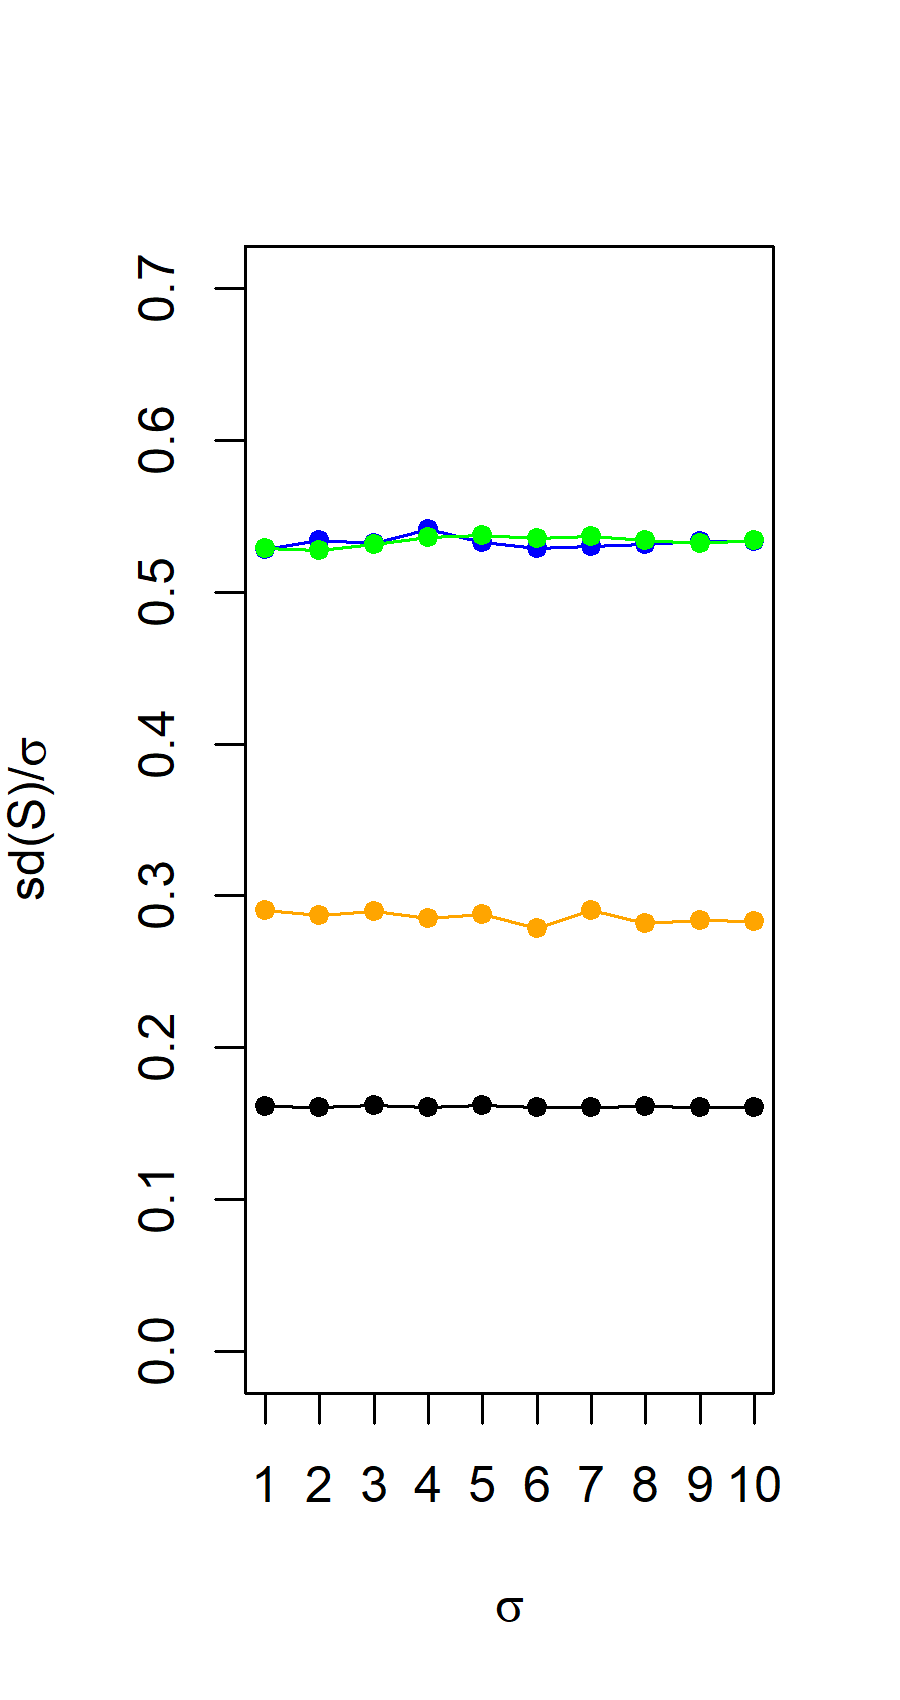
\includegraphics[width=0.2\linewidth]{C:/Users/Marie/Documents/Github_projects/Effect-sizes/Scripts outputs/Quality of ES measures/Graphs/subconditions/hetBal/bias_eff,G1=0 & G2=0;id_sdSD_bal1} \includegraphics[width=0.2\linewidth]{C:/Users/Marie/Documents/Github_projects/Effect-sizes/Scripts outputs/Quality of ES measures/Graphs/subconditions/hetBal/bias_eff,G1=0 & G2=95.75;id_sdSD_bal1} \includegraphics[width=0.2\linewidth]{C:/Users/Marie/Documents/Github_projects/Effect-sizes/Scripts outputs/Quality of ES measures/Graphs/subconditions/hetBal/bias_eff,G1=2.08 & G2=95.75;id_sdSD_bal1} \includegraphics[width=0.2\linewidth]{C:/Users/Marie/Documents/Github_projects/Effect-sizes/Scripts outputs/Quality of ES measures/Graphs/subconditions/hetBal/bias_eff,G1=6.32 & G2=95.75;id_sdSD_bal1} 

}

\caption{Bias and efficiency of estimators, when sample sizes are equal across groups and population variances are unequal, when SD1 is lower than SD2 (condition c2)}\label{fig:idHetbal3}
\end{sidewaysfigure}

Figure \ref{fig:idHetrpos} and \ref{fig:idHetrneg} refer to conditions where there is a pairing between population variances and sample sizes. We know that in these configurations, the pooled variance will be poorly estimated (see the second remark at the beginning of the result section), and therefore, we will not discuss the Cohen's \(d_s\) and Hedge's \(g_s\).We will only compare the quality of Glass's \(d_s\), Shieh's \(d_s\) and Shieh's \(d^*_s\).

Figure \ref{fig:idHetrpos} shows that when variances are unequal, and the largest group is associated with largest variance, the more biased and variable estimator is Glass's \(d_s\) when choosing the standard deviation of the smallest group as standardizer.
REM: AGAIN ONE OBSERVE THE SAME INTERACTION EFFECT BETWEEN STANDARDISER IN GLASS MEASURE AND SENSE OF ASYMMETRY AS OBSERVED FOR FIGURE 3 (IN SAME DIRECTION: WITH NEGATIVE SKEWNESS, WORST WHEN CHOOSING SD1 AND WHEN POSITIVE SKEWNESS, WORST WHEN CHOOSING SD2). Glass's \(d_s\) when choosing the standard deviation of the largest group as standardizer, Shieh's \(d_s\) and transformed Shieh's \(d^*_s\) perform very similarly, both in terms of bias and efficiency.

\begin{sidewaysfigure}

{\centering 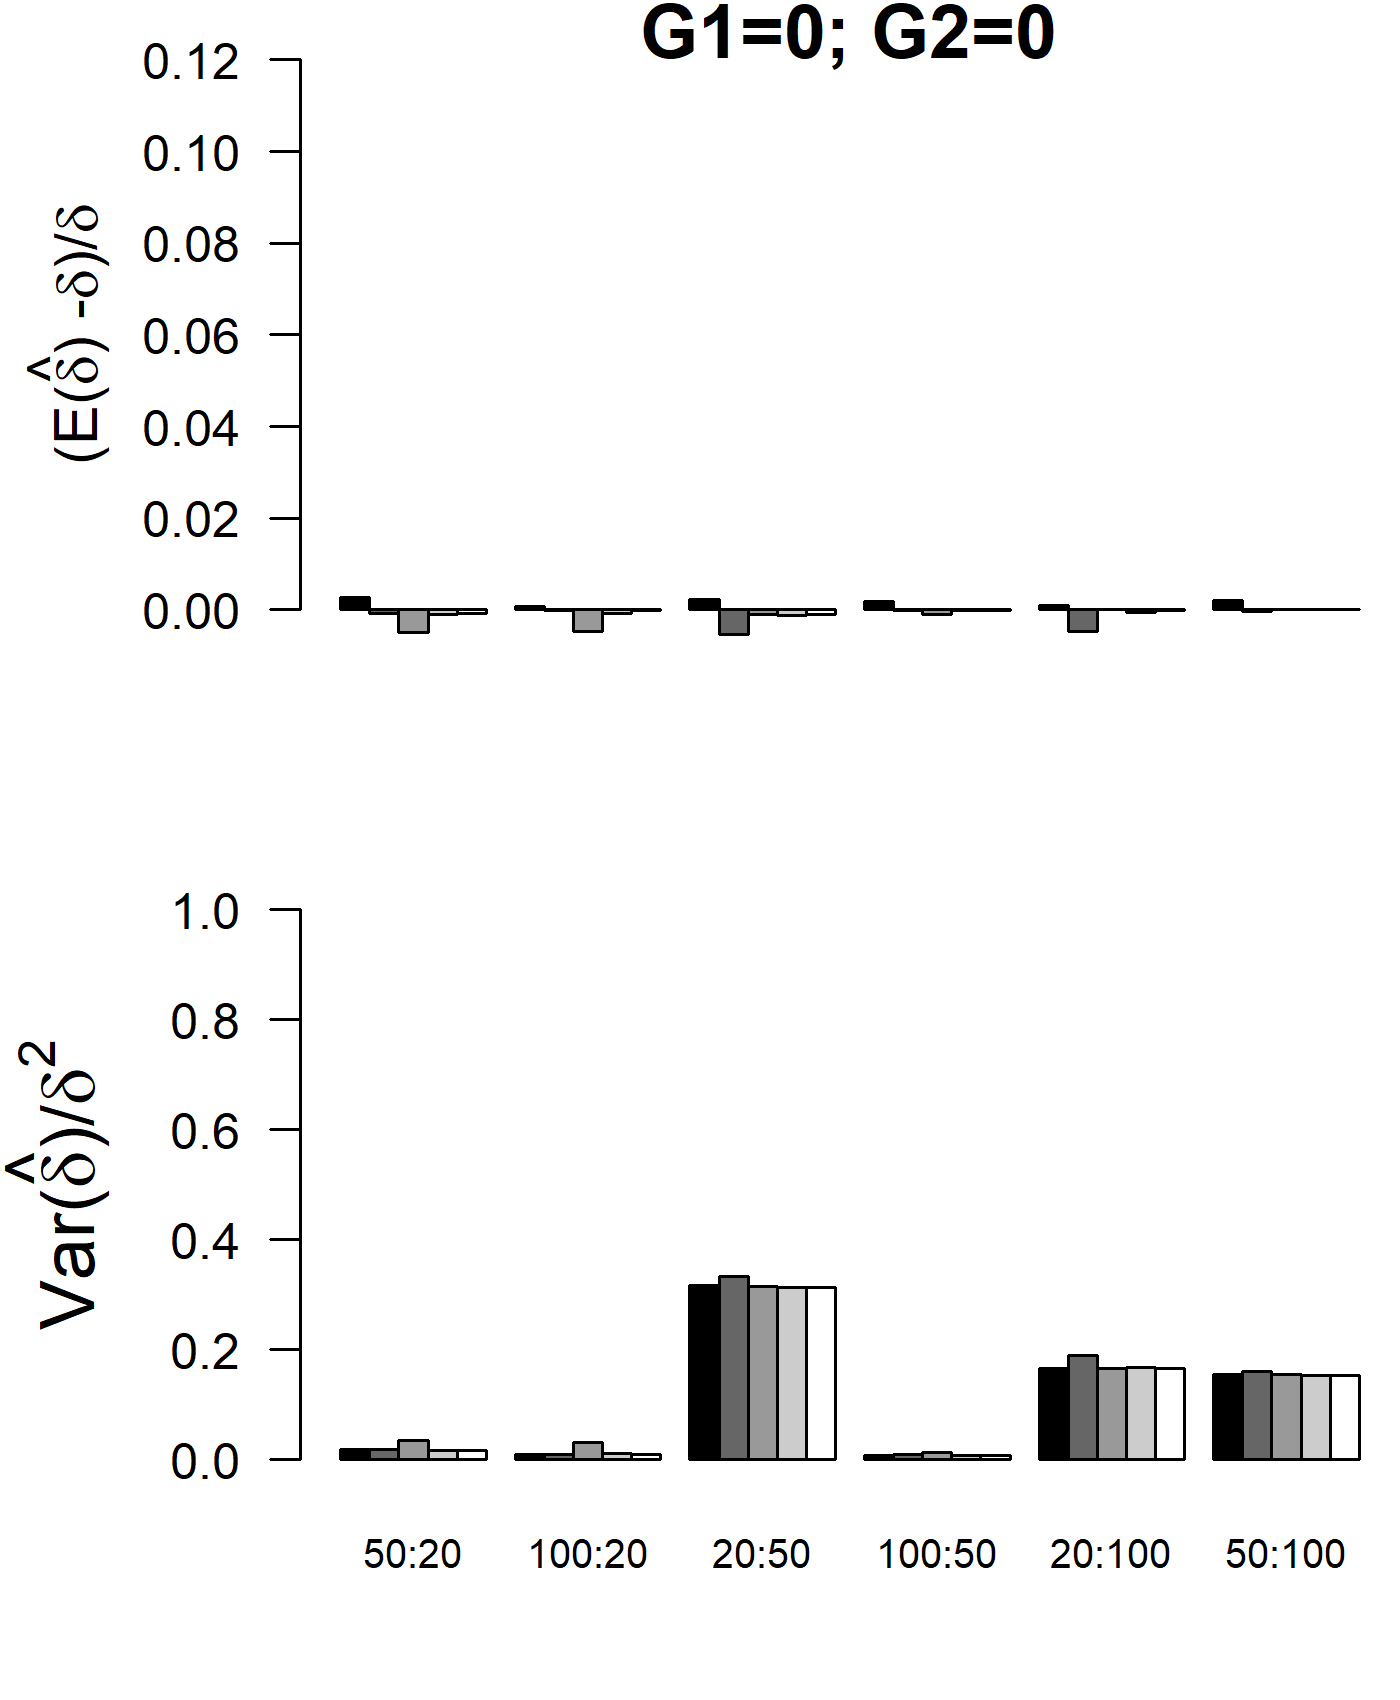
\includegraphics[width=0.2\linewidth]{C:/Users/Marie/Documents/Github_projects/Effect-sizes/Scripts outputs/Quality of ES measures/Graphs/id_Het_rpos/bias_eff,G1=0 & G2=0;id_Het_rpos} 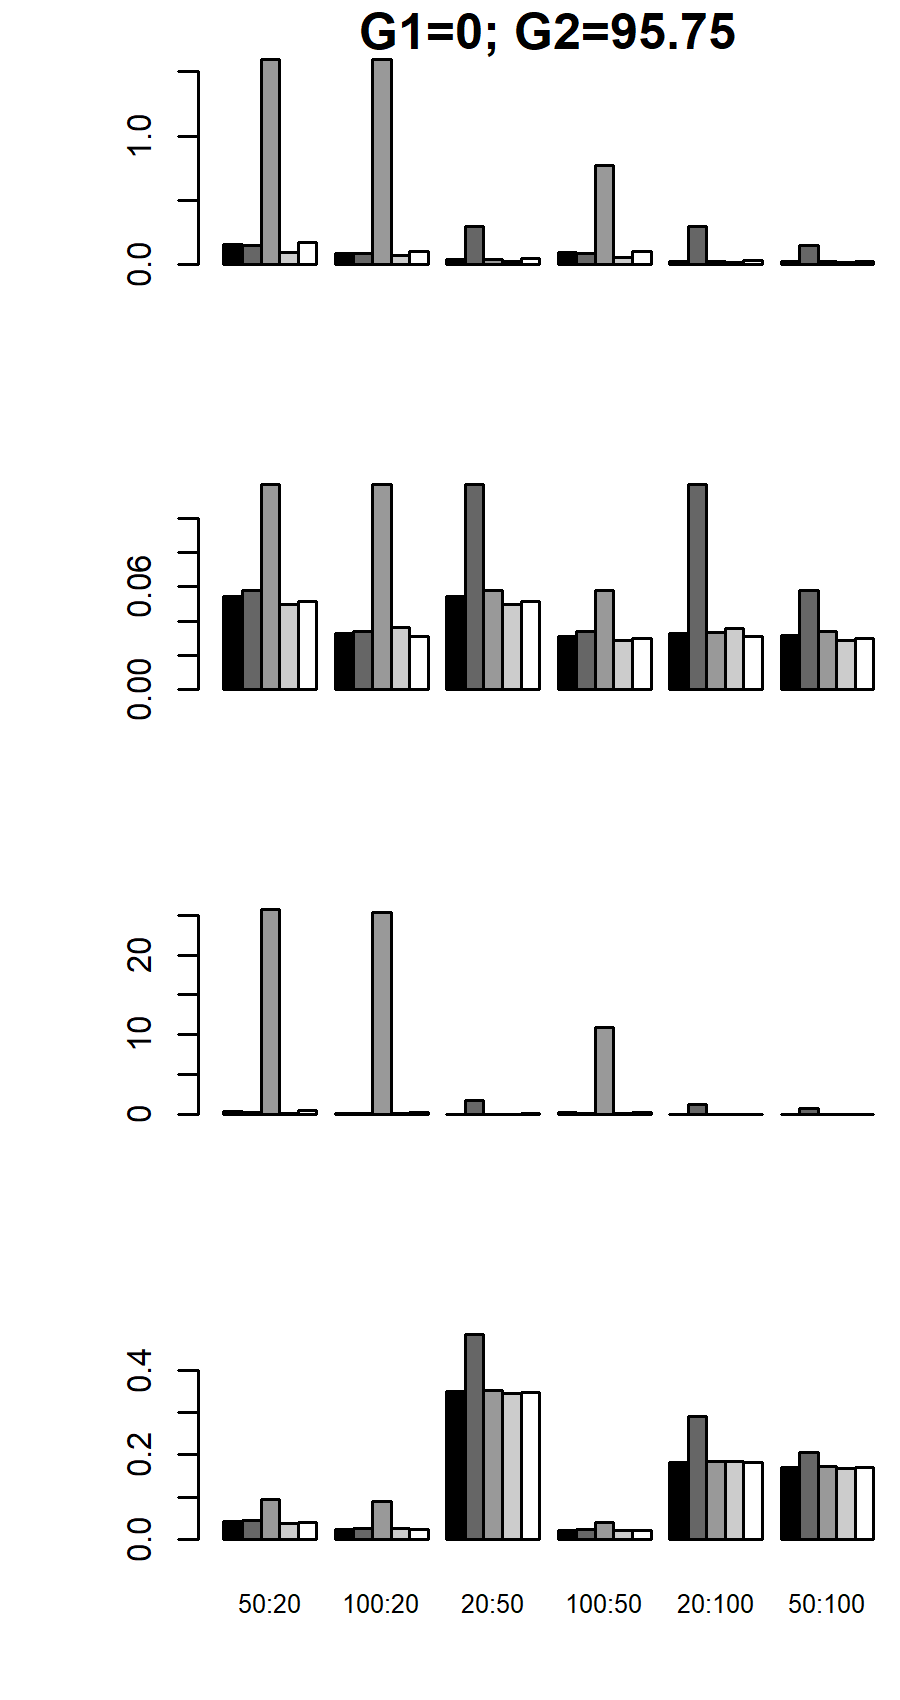
\includegraphics[width=0.2\linewidth]{C:/Users/Marie/Documents/Github_projects/Effect-sizes/Scripts outputs/Quality of ES measures/Graphs/id_Het_rpos/bias_eff,G1=0 & G2=95.75;id_Het_rpos} 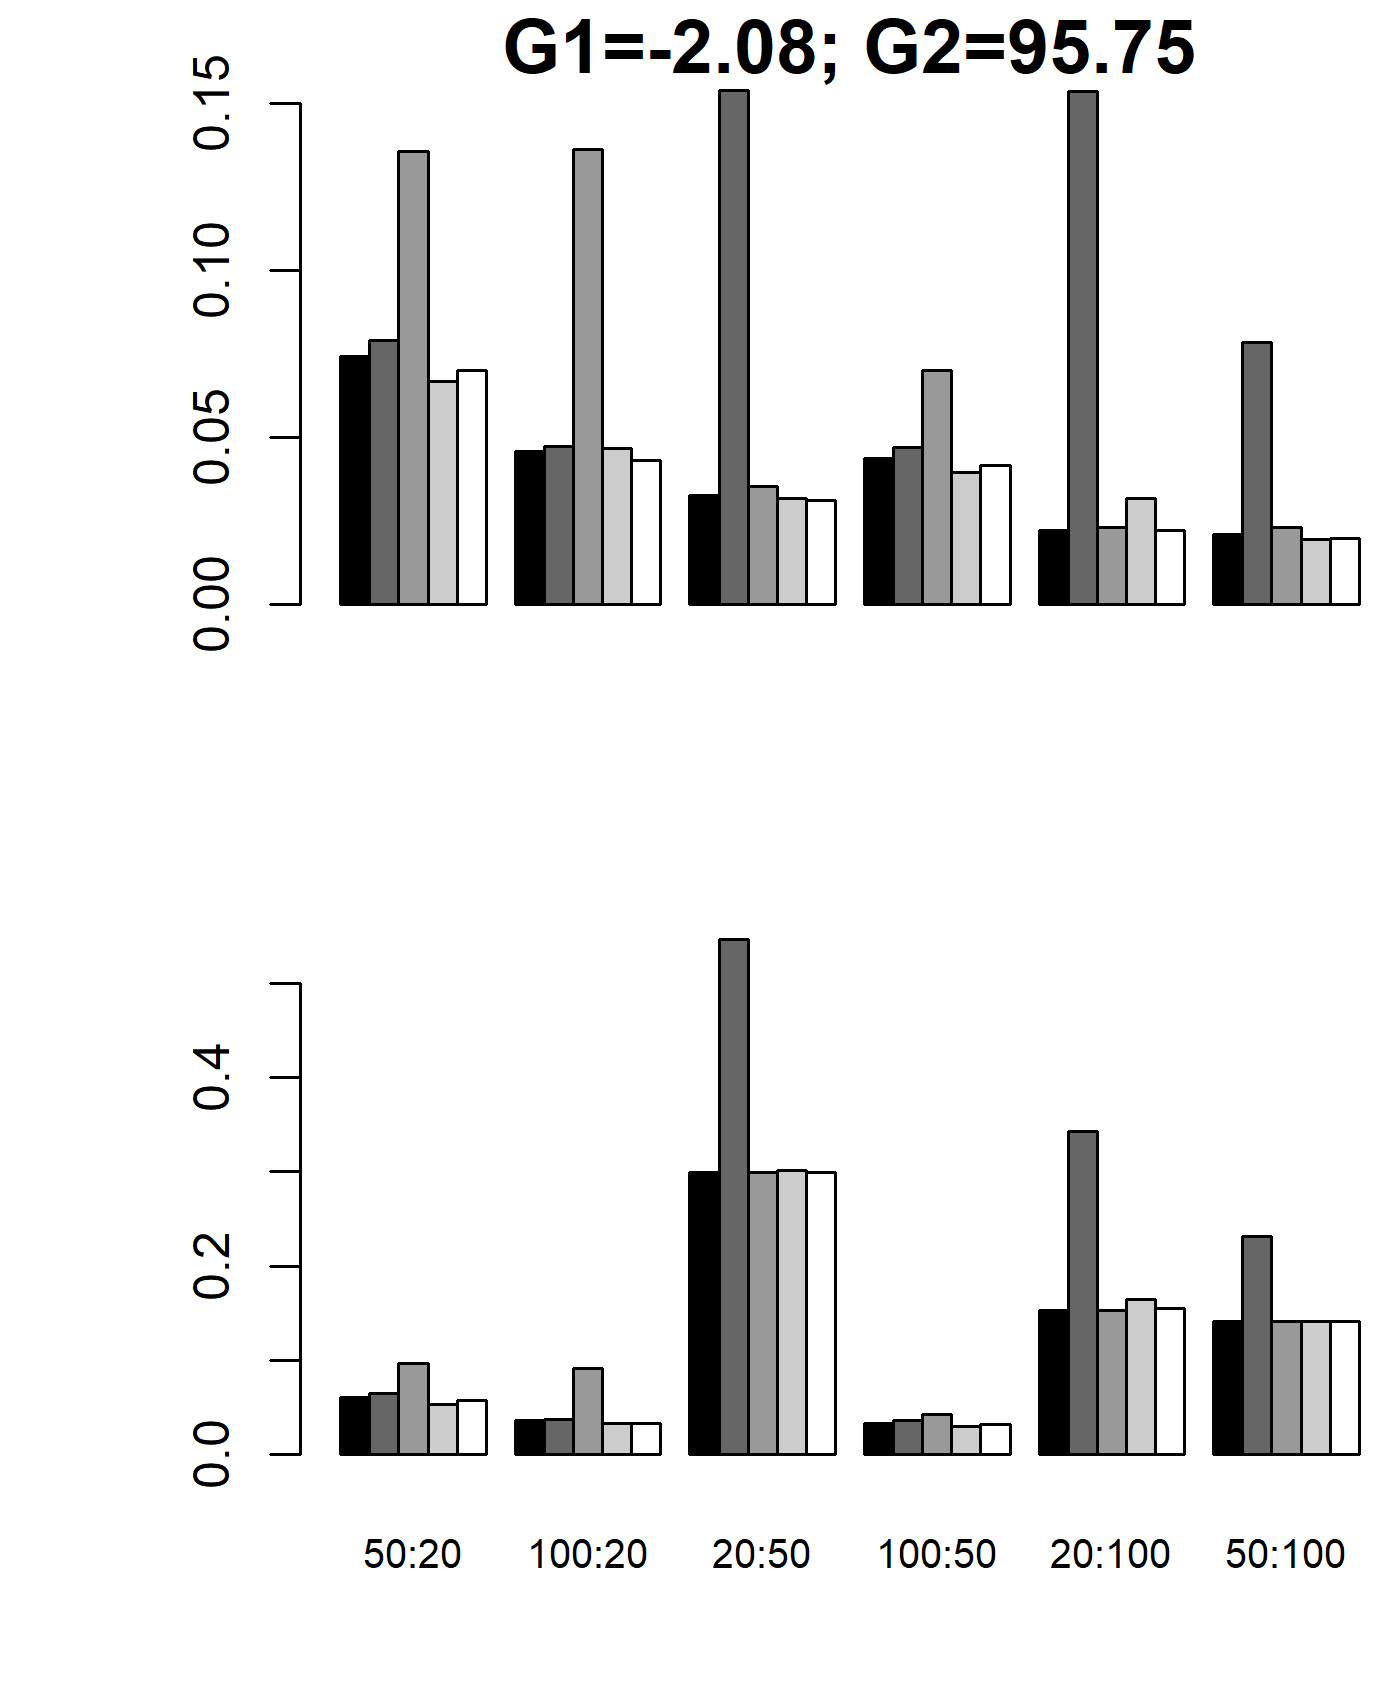
\includegraphics[width=0.2\linewidth]{C:/Users/Marie/Documents/Github_projects/Effect-sizes/Scripts outputs/Quality of ES measures/Graphs/id_Het_rpos/bias_eff,G1=2.08 & G2=95.75;id_Het_rpos} 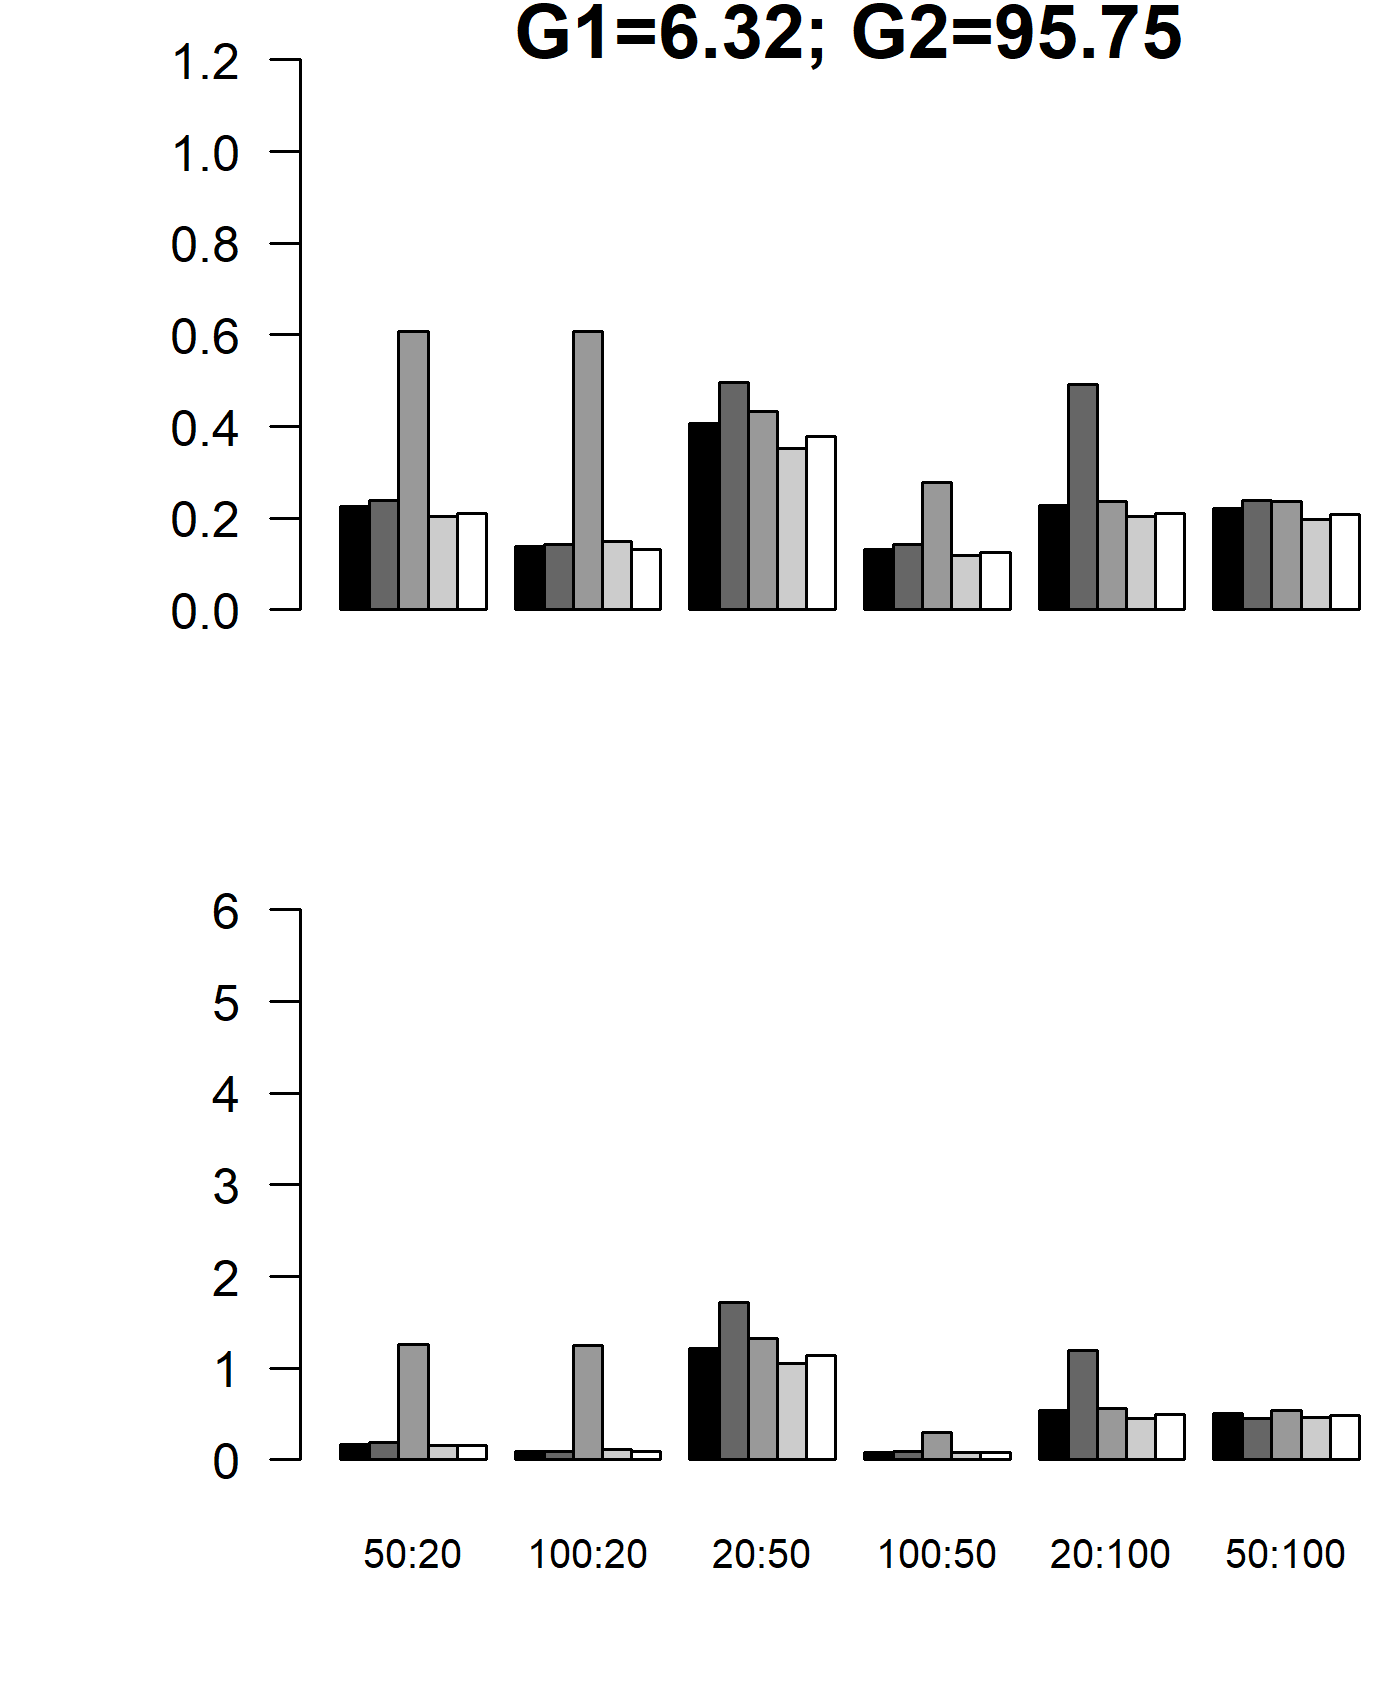
\includegraphics[width=0.2\linewidth]{C:/Users/Marie/Documents/Github_projects/Effect-sizes/Scripts outputs/Quality of ES measures/Graphs/id_Het_rpos/bias_eff,G1=6.32 & G2=95.75;id_Het_rpos} 

}

\caption{Bias and efficiency of estimators of standardized mean difference, when variances and sample sizes are unequal across groups, with positive correlation between them (condition d)}\label{fig:idHetrpos}
\end{sidewaysfigure}

Figure \ref{fig:idHetrneg} shows that when variances are unequal, and the largest group is associated with smallest variance, as in all other configurations, the more biased and variable estimator is Glass's \(d_s\) when choosing the standard deviation of the smallest group as standardizer (sauf quand asymetrie négative\ldots{} not true anymore when there is asymmetry\ldots{} explain it).

\begin{sidewaysfigure}

{\centering 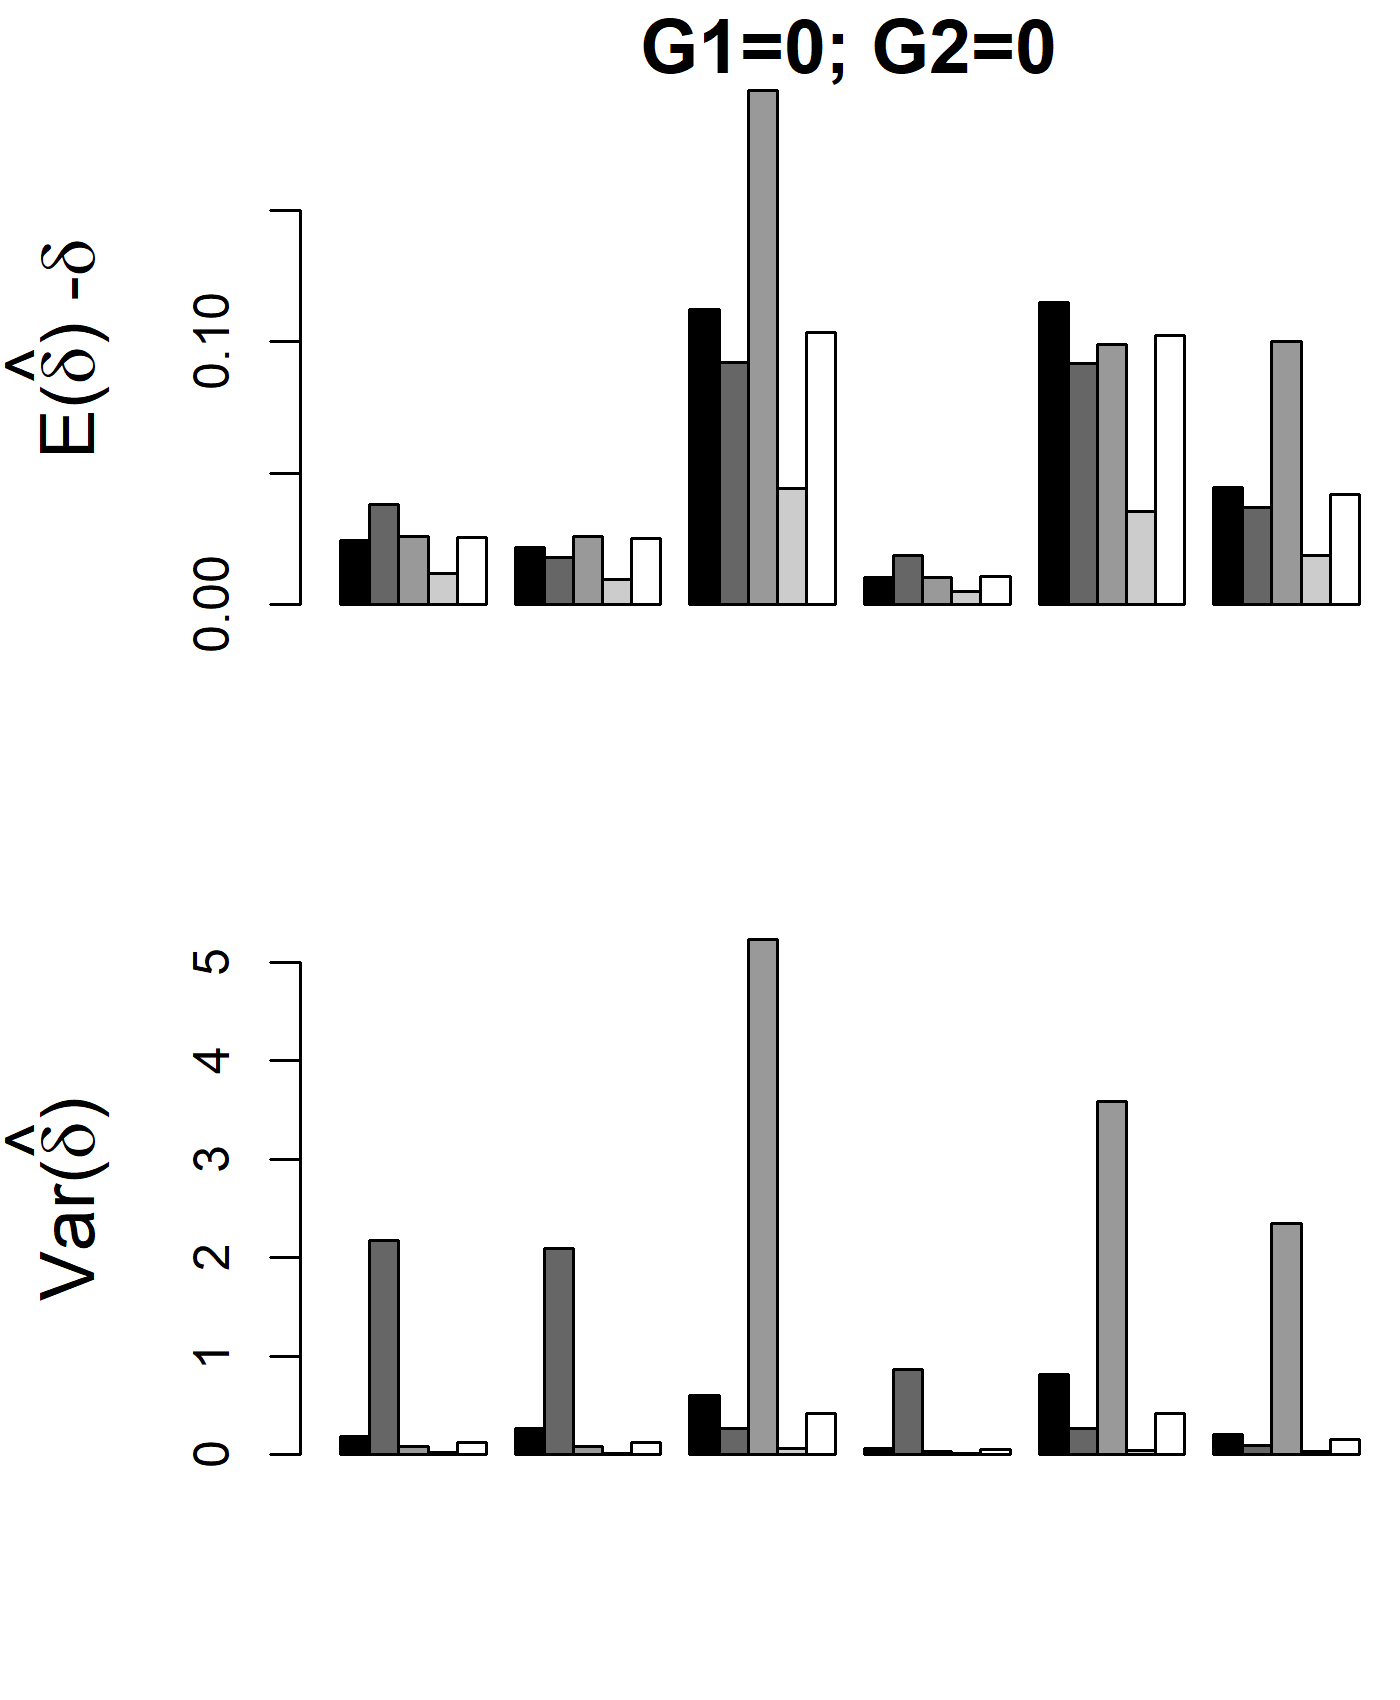
\includegraphics[width=0.2\linewidth]{C:/Users/Marie/Documents/Github_projects/Effect-sizes/Scripts outputs/Quality of ES measures/Graphs/id_Het_rneg/bias_eff,G1=0 & G2=0;id_Het_rneg} 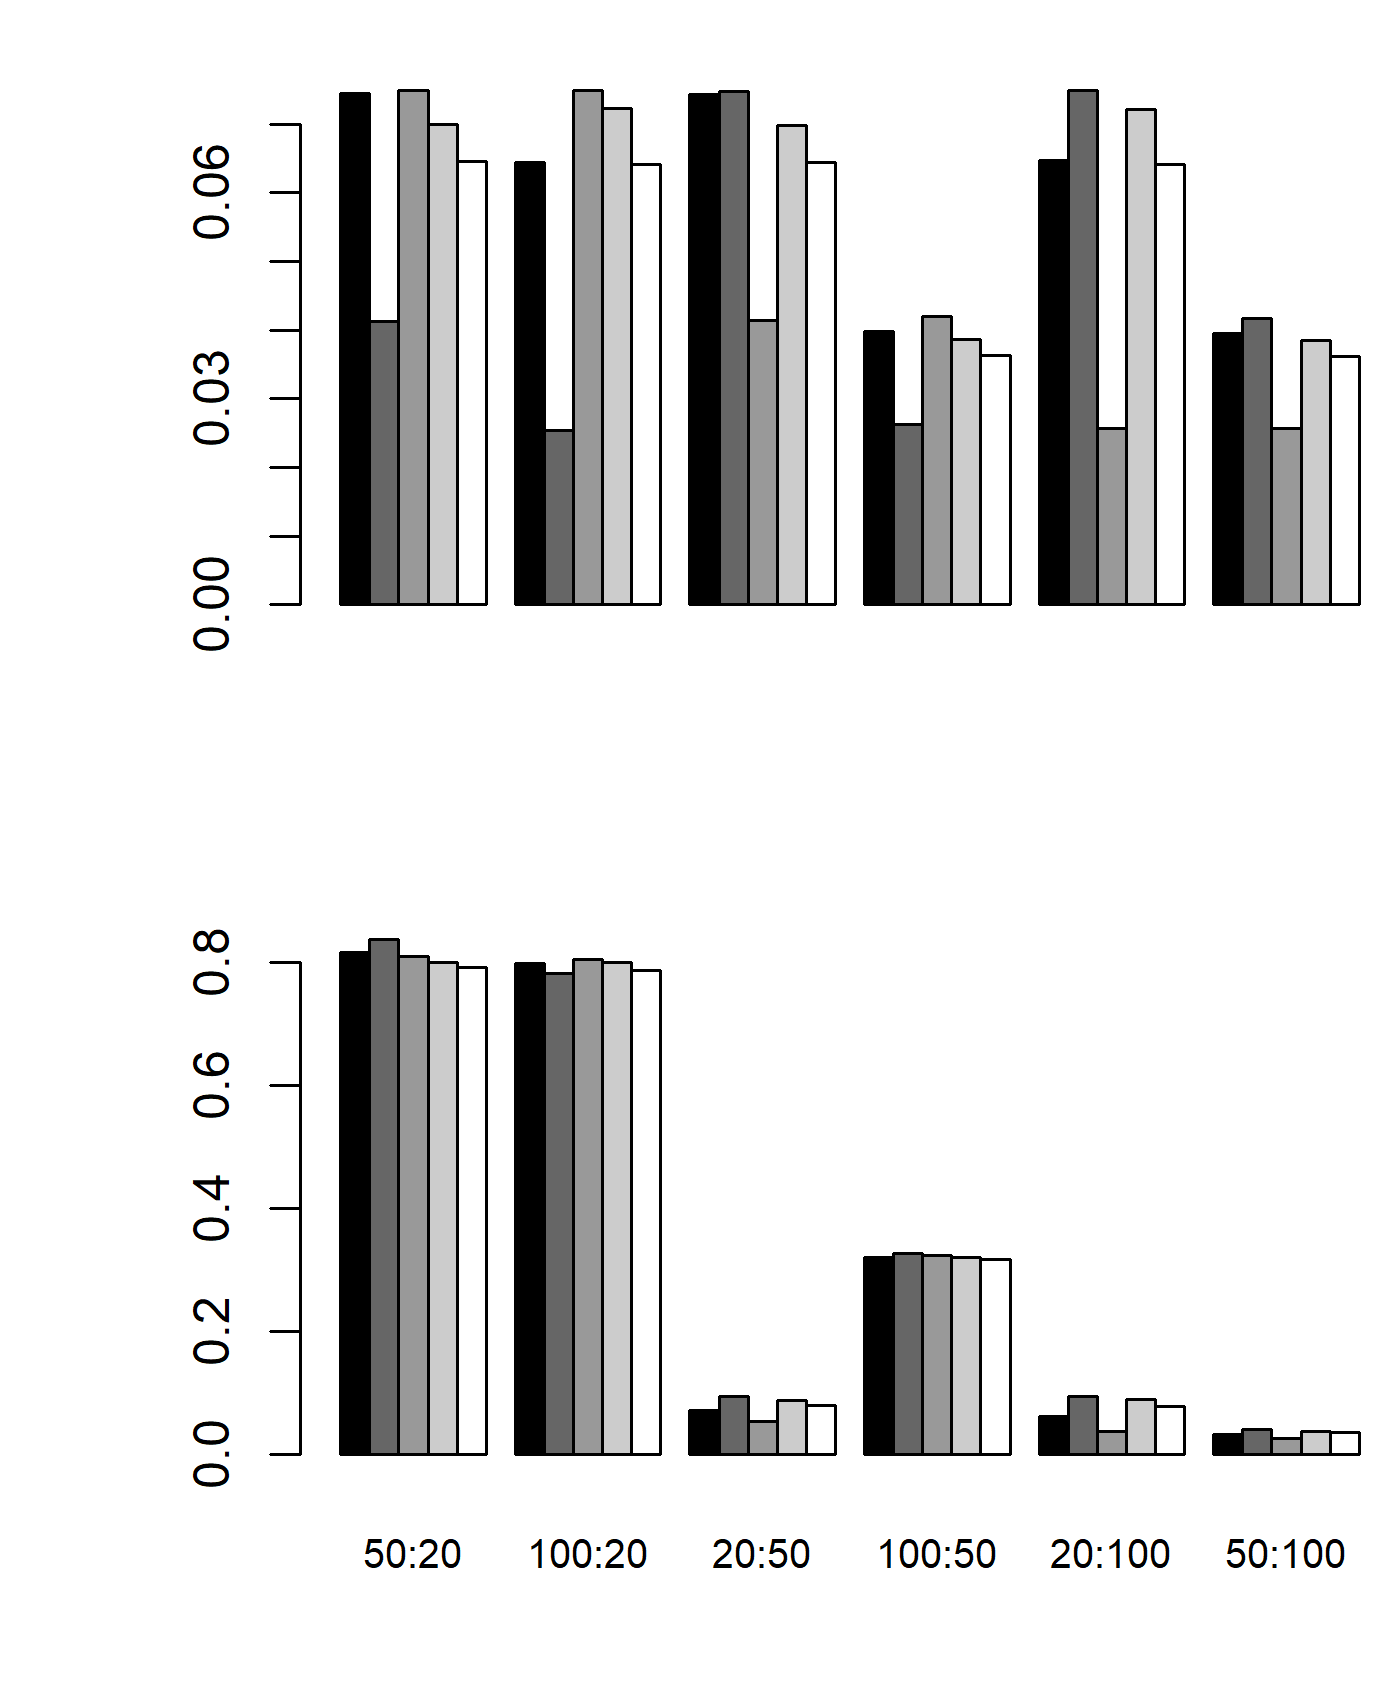
\includegraphics[width=0.2\linewidth]{C:/Users/Marie/Documents/Github_projects/Effect-sizes/Scripts outputs/Quality of ES measures/Graphs/id_Het_rneg/bias_eff,G1=0 & G2=95.75;id_Het_rneg} 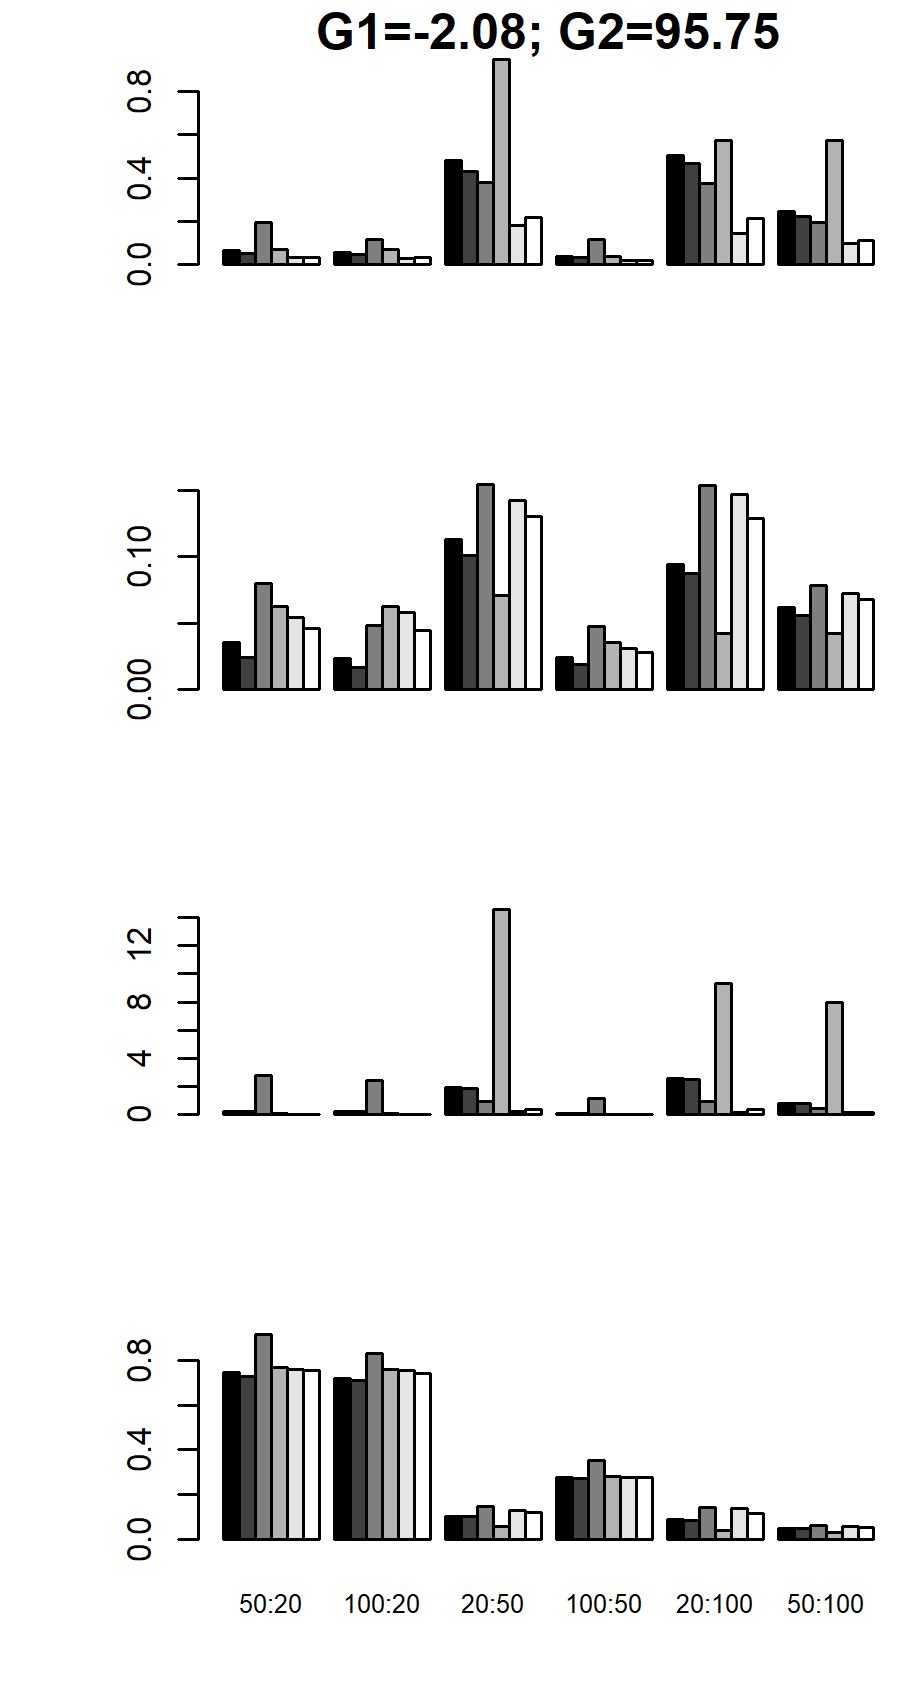
\includegraphics[width=0.2\linewidth]{C:/Users/Marie/Documents/Github_projects/Effect-sizes/Scripts outputs/Quality of ES measures/Graphs/id_Het_rneg/bias_eff,G1=2.08 & G2=95.75;id_Het_rneg} 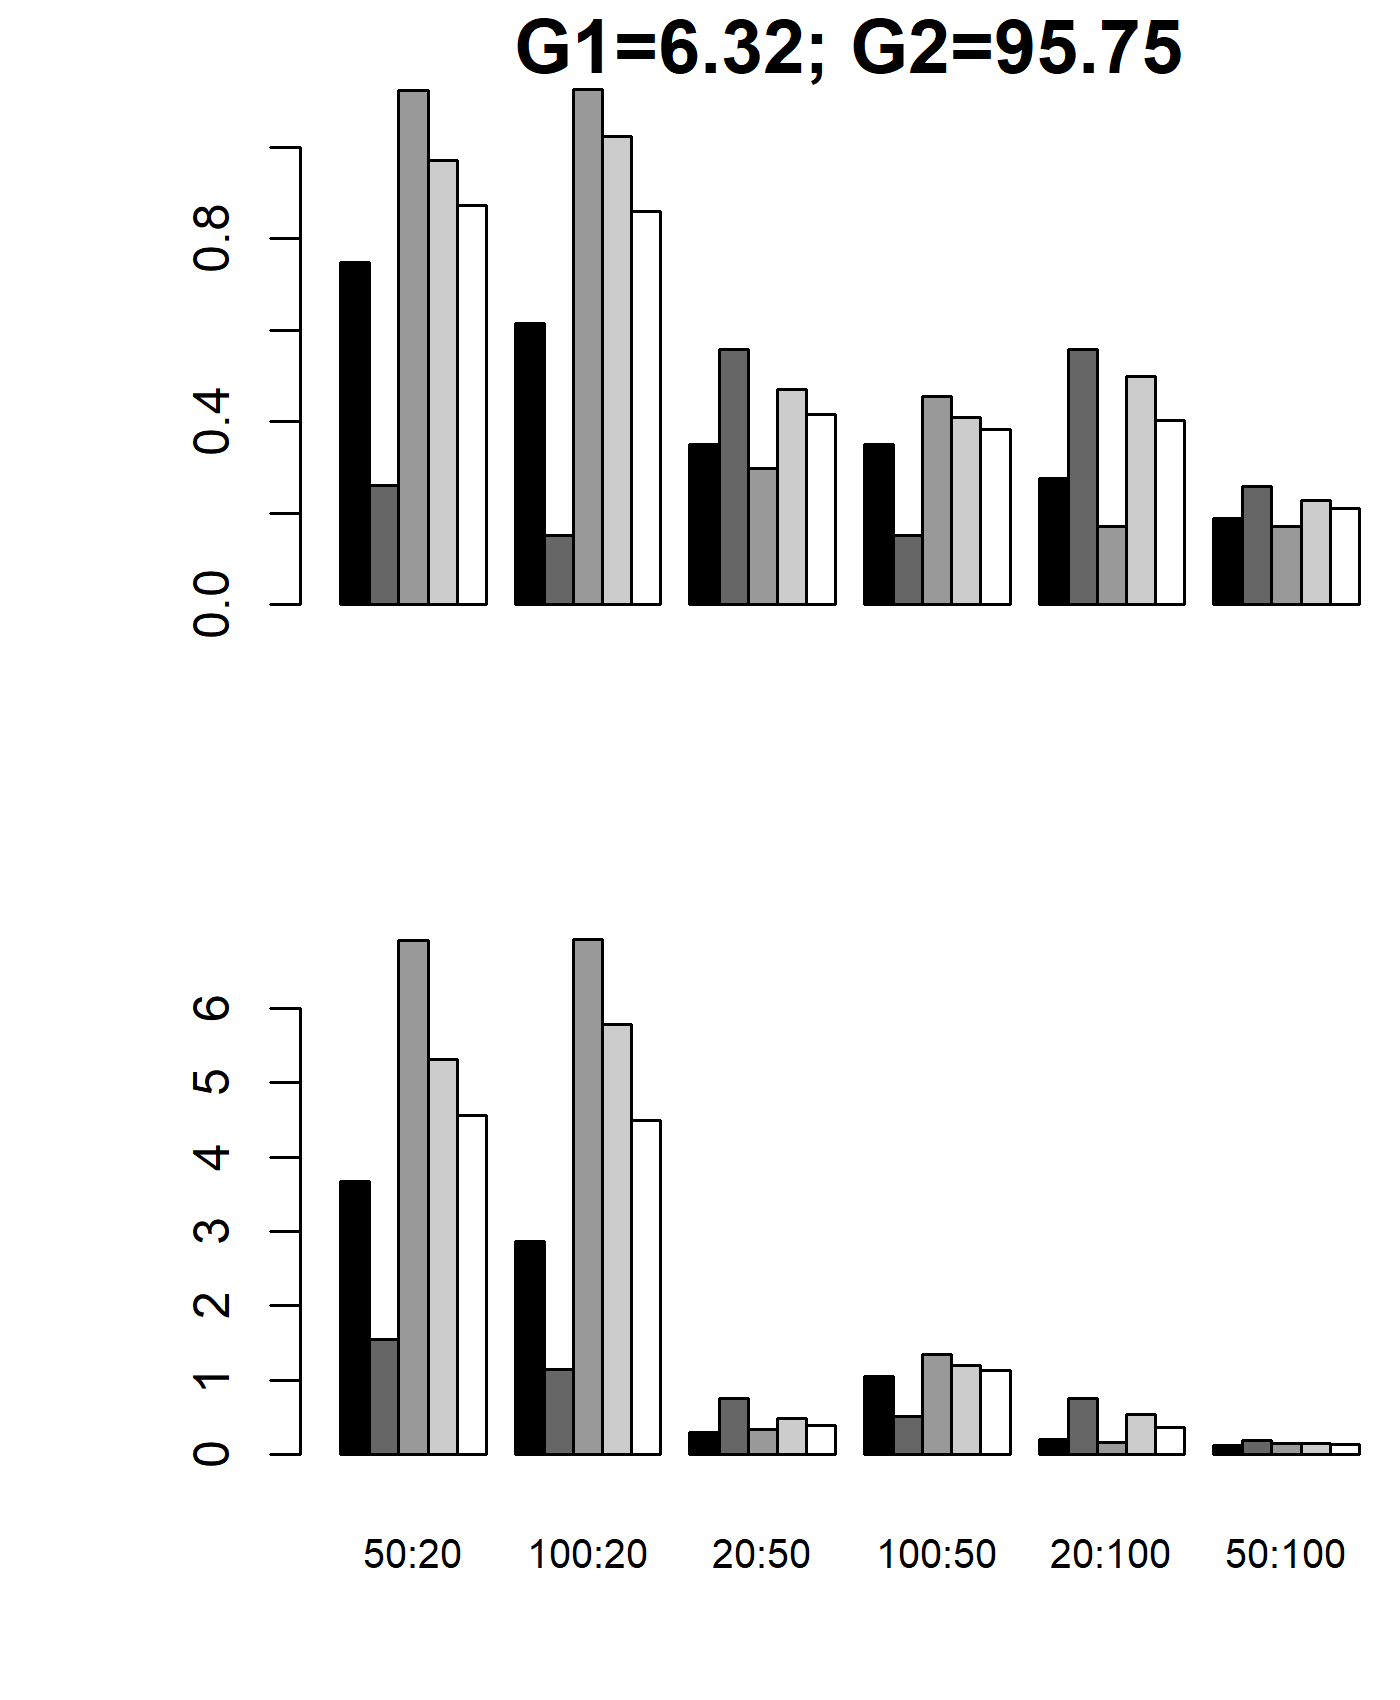
\includegraphics[width=0.2\linewidth]{C:/Users/Marie/Documents/Github_projects/Effect-sizes/Scripts outputs/Quality of ES measures/Graphs/id_Het_rneg/bias_eff,G1=6.32 & G2=95.75;id_Het_rneg} 

}

\caption{Bias and efficiency of estimators of standardized mean difference, when variances and sample sizes are unequal across groups, with negative correlation between them (condition e)}\label{fig:idHetrneg}
\end{sidewaysfigure}

In summary, Cohen's \(d_s\) and Hedge's \(d_s\) remain the best measure when the asssumption of equal variances is met. When variances are unequal across populations, Cohen's \(d_s\) and Hedge's \(g_s\) perform exactly as well as Shieh's \(d_s\) and transformed Shieh's \(d^*_s\), as long as sample sizes are equal across groups. However, when variances and sample sizes are both unequal across groups, Cohen's \(d_s\) and Hedge's \(g_s\) become irrelevant. Glass's \(d_s\) is most of the time the more biased and variable measure. We presume this could be explained by the estimation of the \(SD\) based on a subsample, because the bias is larger when standardizer is estimated based on the smallest group. Only under very specific conditions (when there is a negative correlation between sample sizes and variances and the sample size of the control group is larger than the sample size of the experimental group), Glass's \(d_s\) performs the best in comparison with all other estimators.

\hypertarget{conclusion}{%
\paragraph{Conclusion}\label{conclusion}}

SUMMARY GLASS: il y a plusieurs facteurs \enquote{aggravants}:\\
Pour le biais:
(1) SD calculé sur base du plus petit n (--\textgreater{} mesure plus variable et biaisée car distributions plus asymétrique) --\textgreater{} vrai pour toute distribution
(2) SD négativement corrélé avec la différence de moyenne quand mu1-mu2 \textgreater{} 0 (= choix de SD2 quand asymétrie positive, et de SD1 quand asymétrie négative, vu qu'on calcule m1-m2) OU SD positivement corrélé avec la différence de moyenne quand mu1-mu2 \textless{} 0 (= choix de SD1 quand asymétrie positive, et de SD2 quand asymétrie négative, vu qu'on calcule m1-m2). --\textgreater{} vrai seulement quand distributions asymétriques

Pour la variance:
(1) et (2) jouent, mais il y a en plus:
(3) SD calculé sur base du plus petit sigma

Shieh's \(d_s\) and our transformed Shieh's \(d^*_S\) are the only measure that have an acceptable bias and variance in all configurations. Considering the fact that our transformed Shieh's \(d^*_s\) is much more generalizable (and therefore interpretable) than Shieh \(d_s\), we would recommend the use of this measure in all situations, unless we have very good reason to believe that variances are the same across populations.

\hypertarget{simulation-2-confidence-intervals}{%
\subsubsection{Simulation 2: confidence intervals}\label{simulation-2-confidence-intervals}}

TO DO
\#\#\#\# Method
\#\#\# Results
\#\#\#\# Conclusion

\hypertarget{refs}{}
\leavevmode\hypertarget{ref-Algina_et_al_2006}{}%
Algina, J., Keselman, H. J., \& Penfield, R. D. (2006). Confidence intervals for an effect size when variances are not equal. \emph{Journal of Modern Applied Statistical Methods}, \emph{5}(1), 1--13. doi:\href{https://doi.org/10.22237/jmasm/1146456060}{10.22237/jmasm/1146456060}

\leavevmode\hypertarget{ref-Altman_2005}{}%
Altman, G. D. (2005). Why we need confidence intervals. \emph{World Journal of Surgery}, \emph{29}, 554--556. doi:\href{https://doi.org/10.1007/s00268-005-7911-0}{10.1007/s00268-005-7911-0}

\leavevmode\hypertarget{ref-AERA_2006}{}%
American Educational Research Association. (2006). Standards for reporting on empirical social science research in aera publications. \emph{Educational Researcher}, \emph{35}, 33--40. doi:\href{https://doi.org/10.3102/0013189X035006033}{10.3102/0013189X035006033}

\leavevmode\hypertarget{ref-APA_2010}{}%
American Psychological Association. (2010). \emph{Publication manual of the american psychological association {[}apa{]} (6 ed.)} (American Psychological Association.). Washington, DC:

\leavevmode\hypertarget{ref-Andersen_et_al_2007}{}%
Andersen, M. B., McCullagh, P., \& Wilson, G. J. (2007). But what do the numbers really tell us? Arbitrary metrics and effect size reporting in sport psychology research. \emph{Journal of Sport \& Exercise Psychology}, \emph{29}, 664--672.

\leavevmode\hypertarget{ref-Bothe_Richardson_2011}{}%
Bothe, A. K., \& Richardson, J. D. (2011). Statistical, practical, clinical, and personal significance: Definitions and applications in speech-language pathology. \emph{American Journal of Speech-Language Pathology}, \emph{20}, 233--242.

\leavevmode\hypertarget{ref-Cain_et_al_2017}{}%
Cain, M. K., Zhang, Z., \& Yuan, K.-H. (2017). Univariate and multivariate skewness and kurtosis for measuring nonnormality: Prevalence, influence and estimation. \emph{Behavior Research Methods}, \emph{49}(5), 1716--1735. doi:\href{https://doi.org/10.3758/s13428-016-0814-1}{10.3758/s13428-016-0814-1}

\leavevmode\hypertarget{ref-Coe_2002}{}%
Coe, R. (2002). \emph{It's the effect size, stupid. What effect size is and why it is important}. Retrieved from \url{https://www.leeds.ac.uk/educol/documents/00002182.htm}

\leavevmode\hypertarget{ref-Cohen_1965}{}%
Cohen, J. (1965). Some statistical issues in psychological research. In \emph{Handbook of clinical psychology} (B. B. Wolman., pp. 95--121). New York: McGraw-Hill.

\leavevmode\hypertarget{ref-Cohen_1988}{}%
Cohen, J. (1988). \emph{Statistical power analysis for the behavioral sciences} (Routledge Academic.). New York, NY.

\leavevmode\hypertarget{ref-Cumming_2013}{}%
Cumming, G. (2013). Cohen's d needs to be readily interpretable: Comment on shieh (2013). \emph{Behavior Research Methods}, \emph{45}, 968--971. doi:\href{https://doi.org/10.3758/s13428-013-0392-4}{10.3758/s13428-013-0392-4}

\leavevmode\hypertarget{ref-Delacre_et_al_2017}{}%
Delacre, M., Lakens, D., \& Leys, C. (2017). Why psychologists should by default use welch's t-test instead of student's t-test. \emph{International Review of Social Psychology}, \emph{30}(1), 92--101. doi:\href{https://doi.org/10.5334/irsp.82}{10.5334/irsp.82}

\leavevmode\hypertarget{ref-Delacre_et_al_2019}{}%
Delacre, M., Leys, C., Mora, Y. L., \& Lakens, D. (2019). Taking parametric assumptions seriously: Arguments for the use of welch's f-test instead of the classical f-test in one-way anova. \emph{International Review of Social Psychology}, \emph{32}(1), 1--12. doi:\href{https://doi.org/http://doi.org/10.5334/irsp.198}{http://doi.org/10.5334/irsp.198}

\leavevmode\hypertarget{ref-Ellis_2015}{}%
Ellis, P. D. (2015). \emph{The Essential Guide to Effect Sizes: Statistical Power, Meta-Analysis, and the Interpretation of Research Results} (Cambridge University Press.). Cambridge, UK.

\leavevmode\hypertarget{ref-Erceg-Hurn_Mirosevich_2008}{}%
Erceg-Hurn, D. M., \& Mirosevich, V. M. (2008). Modern robust statistical methods: An easy way to maximize the accuracy and power of your research. \emph{American Psychologist}, \emph{63}(7), 591--601. doi:\href{https://doi.org/10.1037/0003-066X.63.7.591}{10.1037/0003-066X.63.7.591}

\leavevmode\hypertarget{ref-Fan_2001}{}%
Fan, X. (2001). Statistical significance and effect size in education research: Two sides of a coin. \emph{Journal of Educational Research}, \emph{94}(5), 275--282. doi:\href{https://doi.org/10.1080/00220670109598763}{10.1080/00220670109598763}

\leavevmode\hypertarget{ref-Glass_et_al_1981}{}%
Glass, G. V., McGav, B., \& Smith, M. L. (2005). \emph{Meta-analysis in social research} (Sage.). Beverly Hills, CA.

\leavevmode\hypertarget{ref-Glass_et_al_1972}{}%
Glass, G. V., Peckham, P. D., \& Sanders, J. R. (1972). Consequences of failure to meet assumptions underlying the fixed effects analyses of variance and covariance. \emph{Review of Educational Research}, \emph{42}(3), 237--288. doi:\href{https://doi.org/10.3102/00346543042003237}{10.3102/00346543042003237}

\leavevmode\hypertarget{ref-Grissom_2000}{}%
Grissom, R. J. (2000). Heterogeneity of variance in clinical data. \emph{Journal of Consulting and Clinical Psychology}, \emph{68}(1), 155--165. doi:\href{https://doi.org/10.1037//0022-006x.68.1.155}{10.1037//0022-006x.68.1.155}

\leavevmode\hypertarget{ref-Grissom_Kim_2001}{}%
Grissom, R. J., \& Kim, J. J. (2001). Review of assumptions and problems in the appropriate conceptualization of effect size. \emph{Psychological Methods}, \emph{6}(2), 135--146. doi:\href{https://doi.org/10.1037/1082-989X.6.2.135}{10.1037/1082-989X.6.2.135}

\leavevmode\hypertarget{ref-Grissom_and_Kim_2012}{}%
Grissom, R. J., \& Kim, J. J. (2012). \emph{Effect size for research} (Routledges.). New York, NY.

\leavevmode\hypertarget{ref-Grissom_and_kim_2005}{}%
Grissom, R. R., \& Kim, J. J. (2005). \emph{Effect size for research: A broad practical approach.} (Lawrence Erlbaum Associates, Mahwah, N.J.). London.

\leavevmode\hypertarget{ref-Hays_1963}{}%
Hays, W. L. (1963). \emph{Statistics for psychologists} (Holt, Rinehart \& Winston.). New York.

\leavevmode\hypertarget{ref-Hedges_Olkin_1985}{}%
Hedges, L. V., \& Olkin, I. (1985). \emph{Statistical methods for meta-analysis} (Academic Press.). Cambridge, Massachusetts. doi:\href{https://doi.org/10.1016/C2009-0-03396-0}{10.1016/C2009-0-03396-0}

\leavevmode\hypertarget{ref-Henson_Smith_2000}{}%
Henson, R. I., \& Smith, A. D. (2000). State of the art in statistical significance and effect size reporting: A review of the APA task force report and current trends. \emph{Journal of Research and Development in Education}, \emph{33}(4), 285--296.

\leavevmode\hypertarget{ref-Kelley_2005}{}%
Kelley, K. (2005). The effects of nonnormal distributions on confidence intervales around the standardized mean difference: Bootstrap and parametric confidence intervals. \emph{Educational and Psychological Measurement}, \emph{65}(1), 51--69. doi:\href{https://doi.org/10.1177/0013164404264850}{10.1177/0013164404264850}

\leavevmode\hypertarget{ref-Keselman_et_al_2008}{}%
Keselman, H. J., Algina, J., Lix, L. M., Deering, K. N., \& Wilcox, R. R. (2008). A generally robust approach for testing hypotheses and setting confidence intervals for effect sizes. \emph{Psychological Methods}, \emph{13}(2), 110--129. doi:\href{https://doi.org/10.1037/1082-989X.13.2.110}{10.1037/1082-989X.13.2.110}

\leavevmode\hypertarget{ref-Kirk_2009}{}%
Kirk, R. E. (2009). Practical significance: A concept whose time has come. \emph{Educational and Psychological Measurement}, \emph{56}(5), 746--759. doi:\href{https://doi.org/10.1177/0013164496056005002\%20}{10.1177/0013164496056005002 }

\leavevmode\hypertarget{ref-Kulinskaya_Staudte_2007}{}%
Kulinskaya, E., \& Staudte, R. G. (2007). Confidence intervals for the standardized effect arising in the comparison of two normal populations. \emph{Statistics In Medicine}, \emph{26}, 2853--2871. doi:\href{https://doi.org/10.1002/sim.2751}{10.1002/sim.2751}

\leavevmode\hypertarget{ref-Lakens_2013}{}%
Lakens, D. (2013). Calculating and reporting effect sizes to facilitate cumulative science: A practical primer for t-tests and ANOVAs. \emph{Frontiers in Psychology}, \emph{4}(863), 1--12. doi:\href{https://doi.org/10.3389/fpsyg.2013.00863}{10.3389/fpsyg.2013.00863}

\leavevmode\hypertarget{ref-Li_2016}{}%
Li, J. (2016). Effect size measures in a two-independent-samples case with nonnormal and nonhomogeneous data. \emph{Behavior Research Methods}, \emph{48}(4), 1560--1574. doi:\href{https://doi.org/10.3758/s13428-015-0667-z}{10.3758/s13428-015-0667-z}

\leavevmode\hypertarget{ref-McBride_et_al_1993}{}%
McBride, G. B., Loftis, J. C., \& Adkins, N. C. (1993). What do significance tests really tell us about the environment? \emph{Environmental Management}, \emph{17}(4), 423--432.

\leavevmode\hypertarget{ref-Meehl_1990}{}%
Meehl, P. E. (1990). Appraising and amending theories: The strategy of Lakatosian defense and two principles that warrant it. \emph{Psychological Inquiry}, \emph{1}(2), 108--141.

\leavevmode\hypertarget{ref-Micceri_1989}{}%
Micceri, T. (1989). The unicorn, the normal curve, and other improbable creatures. \emph{Psychological Bulletin}, \emph{105}(1), 156--166. doi:\href{https://doi.org/10.1037/0033-2909.105.1.156}{10.1037/0033-2909.105.1.156}

\leavevmode\hypertarget{ref-Nakagawa_and_Cuthill_2007}{}%
Nakagawa, S., \& Cuthill, I. C. (2007). Effect size, confidence interval and statistical significance: A practical guide for biologists. \emph{Biological Reviews}, \emph{82}, 591--605. doi:\href{https://doi.org/10.1111/j.1469-185X.2007.00027.x}{10.1111/j.1469-185X.2007.00027.x}

\leavevmode\hypertarget{ref-Olejnik_Algina_2000}{}%
Olejnik, S., \& Algina, J. (2000). Measures of effect size for comparative studies: Applications, interpretations, and limitations. \emph{Contemporary Educational Psychology}, \emph{25}, 241--286. doi:\href{https://doi.org/10.1006/ceps.2000.1040}{10.1006/ceps.2000.1040}

\leavevmode\hypertarget{ref-Peng_and_Chen_2014}{}%
Peng, C.-Y., \& Chen, L.-T. (2014). Beyond cohen's d: Alternative effect size measures for between-subject designs. \emph{THE JOURNAL OF EXPERIMENTAL EDUCATION}, \emph{82}(1), 22--50. doi:\href{https://doi.org/10.1080/00220973.2012.745471}{10.1080/00220973.2012.745471}

\leavevmode\hypertarget{ref-Peng_et_al_2013}{}%
Peng, C.-Y., Chen, L.-T., Chiang, H.-M., \& Chiang, Y.-C. (2013). The Impact of APA and AERA Guidelines on Effect size Reporting. \emph{Contemporary Educational Psychology}, \emph{82}(1), 22--50. doi:\href{https://doi.org/10.1080/00220973.2012.745471}{10.1080/00220973.2012.745471}

\leavevmode\hypertarget{ref-Prentice_Miller_1992}{}%
Prentice, D., \& Miller, D. T. (1990). When small effects are impressive. \emph{Psychological Bulletin}, \emph{112}(1), 160--164.

\leavevmode\hypertarget{ref-Raviv}{}%
Raviv, E. (2014). \emph{Bias vs. Consistency}. Retrieved March 25, 2020, from \url{https://eranraviv.com/bias-vs-consistency/}

\leavevmode\hypertarget{ref-Rosenthal_1994}{}%
Rosenthal, R. (1994). Parametric measures of effect size. In H. Cooper \& L. V. Hedges (Eds.), \emph{The hand-book of research synthesis} (pp. 231--244). New-York: Sage.

\leavevmode\hypertarget{ref-Shieh_2013}{}%
Shieh, G. (2013). Confidence intervals and sample size calculations for the weighted eta-squared effect sizes in one-way heteroscedastic ANOVA. \emph{Behavior Research Methods}, \emph{45}(1), 2--37. doi:\href{https://doi.org/10.3758/s13428-012-0228-7}{10.3758/s13428-012-0228-7}

\leavevmode\hypertarget{ref-Steyn_2000}{}%
Steyn, H. S. (2000). Practical significance of the difference in means. \emph{Journal of Industrial Psychology}, \emph{26}(3), 1--3.

\leavevmode\hypertarget{ref-Stout_Ruble_1995}{}%
Stout, D. D., \& Ruble, T. L. (1995). Assessing the practical signficance of empirical results in accounting education research: The use of effect size information. \emph{Journal of Accounting Education}, \emph{13}(3), 281--298.

\leavevmode\hypertarget{ref-Sullivan_Feinn_2012}{}%
Sullivan, G., \& Feinn, R. (2012). Using effect size---or why the p value is not enough. \emph{Journal of Graduate Medical Education}, 279--282. doi:\href{https://doi.org/10.4300/JGME-D-12-00156.1}{10.4300/JGME-D-12-00156.1}

\leavevmode\hypertarget{ref-Thompson_2002}{}%
Thompson, B. (2002). "Statistical","Practical", and "Clinical": How Many Kinds of Significance Do Counselors Need to Consider? \emph{Journal of Counseling \& Development}, \emph{80}, 64--71.

\leavevmode\hypertarget{ref-Tyler_1931}{}%
Tyler, R. W. (1931). What is Statistical Significance? \emph{Educational Research Bulletin}, \emph{X}(5), 115--142.

\leavevmode\hypertarget{ref-Wackerly_et_al_2008}{}%
Wackerly, D. D., Mendenhall, W., \& Scheaffer, R. L. (2008). \emph{Mathematical statistics with applications (7th edition)} (Brooks/Cole, Cengage Learning.). Belmont, USA.

\leavevmode\hypertarget{ref-Welch_1938}{}%
Welch, B. L. (1938). The significance of the difference between two means when the population variances are unequal. \emph{Biometrika}, \emph{29}, 350--362.

\leavevmode\hypertarget{ref-Wilkinson_1999}{}%
Wilkinson, L., \& the Task Force on Statistical Inference. (1999). Statistical methods in psychology journals: Guidelines and explanations. \emph{American Psychologist}, \emph{54}(8), 594--604.

\leavevmode\hypertarget{ref-Yuan_et_al_2004}{}%
Yuan, K.-H., Bentler, P. M., \& Chan, W. (2004). Structural equation modeling with heavy tailed distributions. \emph{Psychometrika}, \emph{69}(3), 421--436. doi:\href{https://doi.org/10.1007/bf02295644}{10.1007/bf02295644}

\leavevmode\hypertarget{ref-Algina_et_al_2006}{}%
Algina, J., Keselman, H. J., \& Penfield, R. D. (2006). Confidence intervals for an effect size when variances are not equal. \emph{Journal of Modern Applied Statistical Methods}, \emph{5}(1), 1--13. doi:\href{https://doi.org/10.22237/jmasm/1146456060}{10.22237/jmasm/1146456060}

\leavevmode\hypertarget{ref-Altman_2005}{}%
Altman, G. D. (2005). Why we need confidence intervals. \emph{World Journal of Surgery}, \emph{29}, 554--556. doi:\href{https://doi.org/10.1007/s00268-005-7911-0}{10.1007/s00268-005-7911-0}

\leavevmode\hypertarget{ref-AERA_2006}{}%
American Educational Research Association. (2006). Standards for reporting on empirical social science research in aera publications. \emph{Educational Researcher}, \emph{35}, 33--40. doi:\href{https://doi.org/10.3102/0013189X035006033}{10.3102/0013189X035006033}

\leavevmode\hypertarget{ref-APA_2010}{}%
American Psychological Association. (2010). \emph{Publication manual of the american psychological association {[}apa{]} (6 ed.)} (American Psychological Association.). Washington, DC:

\leavevmode\hypertarget{ref-Andersen_et_al_2007}{}%
Andersen, M. B., McCullagh, P., \& Wilson, G. J. (2007). But what do the numbers really tell us? Arbitrary metrics and effect size reporting in sport psychology research. \emph{Journal of Sport \& Exercise Psychology}, \emph{29}, 664--672.

\leavevmode\hypertarget{ref-Bothe_Richardson_2011}{}%
Bothe, A. K., \& Richardson, J. D. (2011). Statistical, practical, clinical, and personal significance: Definitions and applications in speech-language pathology. \emph{American Journal of Speech-Language Pathology}, \emph{20}, 233--242.

\leavevmode\hypertarget{ref-Cain_et_al_2017}{}%
Cain, M. K., Zhang, Z., \& Yuan, K.-H. (2017). Univariate and multivariate skewness and kurtosis for measuring nonnormality: Prevalence, influence and estimation. \emph{Behavior Research Methods}, \emph{49}(5), 1716--1735. doi:\href{https://doi.org/10.3758/s13428-016-0814-1}{10.3758/s13428-016-0814-1}

\leavevmode\hypertarget{ref-Coe_2002}{}%
Coe, R. (2002). \emph{It's the effect size, stupid. What effect size is and why it is important}. Retrieved from \url{https://www.leeds.ac.uk/educol/documents/00002182.htm}

\leavevmode\hypertarget{ref-Cohen_1965}{}%
Cohen, J. (1965). Some statistical issues in psychological research. In \emph{Handbook of clinical psychology} (B. B. Wolman., pp. 95--121). New York: McGraw-Hill.

\leavevmode\hypertarget{ref-Cohen_1988}{}%
Cohen, J. (1988). \emph{Statistical power analysis for the behavioral sciences} (Routledge Academic.). New York, NY.

\leavevmode\hypertarget{ref-Cumming_2013}{}%
Cumming, G. (2013). Cohen's d needs to be readily interpretable: Comment on shieh (2013). \emph{Behavior Research Methods}, \emph{45}, 968--971. doi:\href{https://doi.org/10.3758/s13428-013-0392-4}{10.3758/s13428-013-0392-4}

\leavevmode\hypertarget{ref-Delacre_et_al_2017}{}%
Delacre, M., Lakens, D., \& Leys, C. (2017). Why psychologists should by default use welch's t-test instead of student's t-test. \emph{International Review of Social Psychology}, \emph{30}(1), 92--101. doi:\href{https://doi.org/10.5334/irsp.82}{10.5334/irsp.82}

\leavevmode\hypertarget{ref-Delacre_et_al_2019}{}%
Delacre, M., Leys, C., Mora, Y. L., \& Lakens, D. (2019). Taking parametric assumptions seriously: Arguments for the use of welch's f-test instead of the classical f-test in one-way anova. \emph{International Review of Social Psychology}, \emph{32}(1), 1--12. doi:\href{https://doi.org/http://doi.org/10.5334/irsp.198}{http://doi.org/10.5334/irsp.198}

\leavevmode\hypertarget{ref-Ellis_2015}{}%
Ellis, P. D. (2015). \emph{The Essential Guide to Effect Sizes: Statistical Power, Meta-Analysis, and the Interpretation of Research Results} (Cambridge University Press.). Cambridge, UK.

\leavevmode\hypertarget{ref-Erceg-Hurn_Mirosevich_2008}{}%
Erceg-Hurn, D. M., \& Mirosevich, V. M. (2008). Modern robust statistical methods: An easy way to maximize the accuracy and power of your research. \emph{American Psychologist}, \emph{63}(7), 591--601. doi:\href{https://doi.org/10.1037/0003-066X.63.7.591}{10.1037/0003-066X.63.7.591}

\leavevmode\hypertarget{ref-Fan_2001}{}%
Fan, X. (2001). Statistical significance and effect size in education research: Two sides of a coin. \emph{Journal of Educational Research}, \emph{94}(5), 275--282. doi:\href{https://doi.org/10.1080/00220670109598763}{10.1080/00220670109598763}

\leavevmode\hypertarget{ref-Glass_et_al_1981}{}%
Glass, G. V., McGav, B., \& Smith, M. L. (2005). \emph{Meta-analysis in social research} (Sage.). Beverly Hills, CA.

\leavevmode\hypertarget{ref-Glass_et_al_1972}{}%
Glass, G. V., Peckham, P. D., \& Sanders, J. R. (1972). Consequences of failure to meet assumptions underlying the fixed effects analyses of variance and covariance. \emph{Review of Educational Research}, \emph{42}(3), 237--288. doi:\href{https://doi.org/10.3102/00346543042003237}{10.3102/00346543042003237}

\leavevmode\hypertarget{ref-Grissom_2000}{}%
Grissom, R. J. (2000). Heterogeneity of variance in clinical data. \emph{Journal of Consulting and Clinical Psychology}, \emph{68}(1), 155--165. doi:\href{https://doi.org/10.1037//0022-006x.68.1.155}{10.1037//0022-006x.68.1.155}

\leavevmode\hypertarget{ref-Grissom_Kim_2001}{}%
Grissom, R. J., \& Kim, J. J. (2001). Review of assumptions and problems in the appropriate conceptualization of effect size. \emph{Psychological Methods}, \emph{6}(2), 135--146. doi:\href{https://doi.org/10.1037/1082-989X.6.2.135}{10.1037/1082-989X.6.2.135}

\leavevmode\hypertarget{ref-Grissom_and_Kim_2012}{}%
Grissom, R. J., \& Kim, J. J. (2012). \emph{Effect size for research} (Routledges.). New York, NY.

\leavevmode\hypertarget{ref-Grissom_and_kim_2005}{}%
Grissom, R. R., \& Kim, J. J. (2005). \emph{Effect size for research: A broad practical approach.} (Lawrence Erlbaum Associates, Mahwah, N.J.). London.

\leavevmode\hypertarget{ref-Hays_1963}{}%
Hays, W. L. (1963). \emph{Statistics for psychologists} (Holt, Rinehart \& Winston.). New York.

\leavevmode\hypertarget{ref-Hedges_Olkin_1985}{}%
Hedges, L. V., \& Olkin, I. (1985). \emph{Statistical methods for meta-analysis} (Academic Press.). Cambridge, Massachusetts. doi:\href{https://doi.org/10.1016/C2009-0-03396-0}{10.1016/C2009-0-03396-0}

\leavevmode\hypertarget{ref-Henson_Smith_2000}{}%
Henson, R. I., \& Smith, A. D. (2000). State of the art in statistical significance and effect size reporting: A review of the APA task force report and current trends. \emph{Journal of Research and Development in Education}, \emph{33}(4), 285--296.

\leavevmode\hypertarget{ref-Kelley_2005}{}%
Kelley, K. (2005). The effects of nonnormal distributions on confidence intervales around the standardized mean difference: Bootstrap and parametric confidence intervals. \emph{Educational and Psychological Measurement}, \emph{65}(1), 51--69. doi:\href{https://doi.org/10.1177/0013164404264850}{10.1177/0013164404264850}

\leavevmode\hypertarget{ref-Keselman_et_al_2008}{}%
Keselman, H. J., Algina, J., Lix, L. M., Deering, K. N., \& Wilcox, R. R. (2008). A generally robust approach for testing hypotheses and setting confidence intervals for effect sizes. \emph{Psychological Methods}, \emph{13}(2), 110--129. doi:\href{https://doi.org/10.1037/1082-989X.13.2.110}{10.1037/1082-989X.13.2.110}

\leavevmode\hypertarget{ref-Kirk_2009}{}%
Kirk, R. E. (2009). Practical significance: A concept whose time has come. \emph{Educational and Psychological Measurement}, \emph{56}(5), 746--759. doi:\href{https://doi.org/10.1177/0013164496056005002\%20}{10.1177/0013164496056005002 }

\leavevmode\hypertarget{ref-Kulinskaya_Staudte_2007}{}%
Kulinskaya, E., \& Staudte, R. G. (2007). Confidence intervals for the standardized effect arising in the comparison of two normal populations. \emph{Statistics In Medicine}, \emph{26}, 2853--2871. doi:\href{https://doi.org/10.1002/sim.2751}{10.1002/sim.2751}

\leavevmode\hypertarget{ref-Lakens_2013}{}%
Lakens, D. (2013). Calculating and reporting effect sizes to facilitate cumulative science: A practical primer for t-tests and ANOVAs. \emph{Frontiers in Psychology}, \emph{4}(863), 1--12. doi:\href{https://doi.org/10.3389/fpsyg.2013.00863}{10.3389/fpsyg.2013.00863}

\leavevmode\hypertarget{ref-Li_2016}{}%
Li, J. (2016). Effect size measures in a two-independent-samples case with nonnormal and nonhomogeneous data. \emph{Behavior Research Methods}, \emph{48}(4), 1560--1574. doi:\href{https://doi.org/10.3758/s13428-015-0667-z}{10.3758/s13428-015-0667-z}

\leavevmode\hypertarget{ref-McBride_et_al_1993}{}%
McBride, G. B., Loftis, J. C., \& Adkins, N. C. (1993). What do significance tests really tell us about the environment? \emph{Environmental Management}, \emph{17}(4), 423--432.

\leavevmode\hypertarget{ref-Meehl_1990}{}%
Meehl, P. E. (1990). Appraising and amending theories: The strategy of Lakatosian defense and two principles that warrant it. \emph{Psychological Inquiry}, \emph{1}(2), 108--141.

\leavevmode\hypertarget{ref-Micceri_1989}{}%
Micceri, T. (1989). The unicorn, the normal curve, and other improbable creatures. \emph{Psychological Bulletin}, \emph{105}(1), 156--166. doi:\href{https://doi.org/10.1037/0033-2909.105.1.156}{10.1037/0033-2909.105.1.156}

\leavevmode\hypertarget{ref-Nakagawa_and_Cuthill_2007}{}%
Nakagawa, S., \& Cuthill, I. C. (2007). Effect size, confidence interval and statistical significance: A practical guide for biologists. \emph{Biological Reviews}, \emph{82}, 591--605. doi:\href{https://doi.org/10.1111/j.1469-185X.2007.00027.x}{10.1111/j.1469-185X.2007.00027.x}

\leavevmode\hypertarget{ref-Olejnik_Algina_2000}{}%
Olejnik, S., \& Algina, J. (2000). Measures of effect size for comparative studies: Applications, interpretations, and limitations. \emph{Contemporary Educational Psychology}, \emph{25}, 241--286. doi:\href{https://doi.org/10.1006/ceps.2000.1040}{10.1006/ceps.2000.1040}

\leavevmode\hypertarget{ref-Peng_and_Chen_2014}{}%
Peng, C.-Y., \& Chen, L.-T. (2014). Beyond cohen's d: Alternative effect size measures for between-subject designs. \emph{THE JOURNAL OF EXPERIMENTAL EDUCATION}, \emph{82}(1), 22--50. doi:\href{https://doi.org/10.1080/00220973.2012.745471}{10.1080/00220973.2012.745471}

\leavevmode\hypertarget{ref-Peng_et_al_2013}{}%
Peng, C.-Y., Chen, L.-T., Chiang, H.-M., \& Chiang, Y.-C. (2013). The Impact of APA and AERA Guidelines on Effect size Reporting. \emph{Contemporary Educational Psychology}, \emph{82}(1), 22--50. doi:\href{https://doi.org/10.1080/00220973.2012.745471}{10.1080/00220973.2012.745471}

\leavevmode\hypertarget{ref-Prentice_Miller_1992}{}%
Prentice, D., \& Miller, D. T. (1990). When small effects are impressive. \emph{Psychological Bulletin}, \emph{112}(1), 160--164.

\leavevmode\hypertarget{ref-Raviv}{}%
Raviv, E. (2014). \emph{Bias vs. Consistency}. Retrieved March 25, 2020, from \url{https://eranraviv.com/bias-vs-consistency/}

\leavevmode\hypertarget{ref-Rosenthal_1994}{}%
Rosenthal, R. (1994). Parametric measures of effect size. In H. Cooper \& L. V. Hedges (Eds.), \emph{The hand-book of research synthesis} (pp. 231--244). New-York: Sage.

\leavevmode\hypertarget{ref-Shieh_2013}{}%
Shieh, G. (2013). Confidence intervals and sample size calculations for the weighted eta-squared effect sizes in one-way heteroscedastic ANOVA. \emph{Behavior Research Methods}, \emph{45}(1), 2--37. doi:\href{https://doi.org/10.3758/s13428-012-0228-7}{10.3758/s13428-012-0228-7}

\leavevmode\hypertarget{ref-Steyn_2000}{}%
Steyn, H. S. (2000). Practical significance of the difference in means. \emph{Journal of Industrial Psychology}, \emph{26}(3), 1--3.

\leavevmode\hypertarget{ref-Stout_Ruble_1995}{}%
Stout, D. D., \& Ruble, T. L. (1995). Assessing the practical signficance of empirical results in accounting education research: The use of effect size information. \emph{Journal of Accounting Education}, \emph{13}(3), 281--298.

\leavevmode\hypertarget{ref-Sullivan_Feinn_2012}{}%
Sullivan, G., \& Feinn, R. (2012). Using effect size---or why the p value is not enough. \emph{Journal of Graduate Medical Education}, 279--282. doi:\href{https://doi.org/10.4300/JGME-D-12-00156.1}{10.4300/JGME-D-12-00156.1}

\leavevmode\hypertarget{ref-Thompson_2002}{}%
Thompson, B. (2002). "Statistical","Practical", and "Clinical": How Many Kinds of Significance Do Counselors Need to Consider? \emph{Journal of Counseling \& Development}, \emph{80}, 64--71.

\leavevmode\hypertarget{ref-Tyler_1931}{}%
Tyler, R. W. (1931). What is Statistical Significance? \emph{Educational Research Bulletin}, \emph{X}(5), 115--142.

\leavevmode\hypertarget{ref-Wackerly_et_al_2008}{}%
Wackerly, D. D., Mendenhall, W., \& Scheaffer, R. L. (2008). \emph{Mathematical statistics with applications (7th edition)} (Brooks/Cole, Cengage Learning.). Belmont, USA.

\leavevmode\hypertarget{ref-Welch_1938}{}%
Welch, B. L. (1938). The significance of the difference between two means when the population variances are unequal. \emph{Biometrika}, \emph{29}, 350--362.

\leavevmode\hypertarget{ref-Wilkinson_1999}{}%
Wilkinson, L., \& the Task Force on Statistical Inference. (1999). Statistical methods in psychology journals: Guidelines and explanations. \emph{American Psychologist}, \emph{54}(8), 594--604.

\leavevmode\hypertarget{ref-Yuan_et_al_2004}{}%
Yuan, K.-H., Bentler, P. M., \& Chan, W. (2004). Structural equation modeling with heavy tailed distributions. \emph{Psychometrika}, \emph{69}(3), 421--436. doi:\href{https://doi.org/10.1007/bf02295644}{10.1007/bf02295644}

\clearpage
\makeatletter
\efloat@restorefloats
\makeatother


\begin{appendix}
\section{}
\setlength{\parindent}{0.0in}
\setlength{\leftskip}{0.0in}

\hypertarget{appendix-1-the-mathematical-study-of-shiehs-delta}{%
\subsection{\texorpdfstring{Appendix 1: The mathematical study of
Shieh's
\(\delta\)}{Appendix 1: The mathematical study of Shieh's \textbackslash delta}}\label{appendix-1-the-mathematical-study-of-shiehs-delta}}

Paste Appendix 1 when it will be finished

\hypertarget{appendix-2-confidence-intervals}{%
\subsection{Appendix 2: Confidence
intervals}\label{appendix-2-confidence-intervals}}

Paste Appendix 2 when it will be finished

\hypertarget{appendix-3-a-priori-power-analyses}{%
\subsection{Appendix 3: a priori power
analyses}\label{appendix-3-a-priori-power-analyses}}

Paste Appendix 3 when it will be finished (Cumming \& Finch, 2001)

\hypertarget{refs}{}
\leavevmode\hypertarget{ref-Cumming_Finch_2001}{}%
Cumming, G., \& Finch, S. (2001). A primer on the understanding, use,
and calculation of confidence intervales that are based on central and
noncentral distributions. \emph{Educational and Psychological
Measurement}, \emph{61}(532), 532--574.
\end{appendix}

\end{document}
